% Options for packages loaded elsewhere
\PassOptionsToPackage{unicode}{hyperref}
\PassOptionsToPackage{hyphens}{url}
\PassOptionsToPackage{dvipsnames,svgnames,x11names}{xcolor}
%
\documentclass[
  9pt,
  a4paper,
  numbers=noendperiod,
  DIV=12]{scrartcl}

\usepackage{amsmath,amssymb}
\usepackage{lmodern}
\usepackage{iftex}
\ifPDFTeX
  \usepackage[T1]{fontenc}
  \usepackage[utf8]{inputenc}
  \usepackage{textcomp} % provide euro and other symbols
\else % if luatex or xetex
  \usepackage{unicode-math}
  \defaultfontfeatures{Scale=MatchLowercase}
  \defaultfontfeatures[\rmfamily]{Ligatures=TeX,Scale=1}
  \setmainfont[]{Roboto}
\fi
% Use upquote if available, for straight quotes in verbatim environments
\IfFileExists{upquote.sty}{\usepackage{upquote}}{}
\IfFileExists{microtype.sty}{% use microtype if available
  \usepackage[]{microtype}
  \UseMicrotypeSet[protrusion]{basicmath} % disable protrusion for tt fonts
}{}
\makeatletter
\@ifundefined{KOMAClassName}{% if non-KOMA class
  \IfFileExists{parskip.sty}{%
    \usepackage{parskip}
  }{% else
    \setlength{\parindent}{0pt}
    \setlength{\parskip}{6pt plus 2pt minus 1pt}}
}{% if KOMA class
  \KOMAoptions{parskip=half}}
\makeatother
\usepackage{xcolor}
\setlength{\emergencystretch}{3em} % prevent overfull lines
\setcounter{secnumdepth}{1}
% Make \paragraph and \subparagraph free-standing
\ifx\paragraph\undefined\else
  \let\oldparagraph\paragraph
  \renewcommand{\paragraph}[1]{\oldparagraph{#1}\mbox{}}
\fi
\ifx\subparagraph\undefined\else
  \let\oldsubparagraph\subparagraph
  \renewcommand{\subparagraph}[1]{\oldsubparagraph{#1}\mbox{}}
\fi


\providecommand{\tightlist}{%
  \setlength{\itemsep}{0pt}\setlength{\parskip}{0pt}}\usepackage{longtable,booktabs,array}
\usepackage{calc} % for calculating minipage widths
% Correct order of tables after \paragraph or \subparagraph
\usepackage{etoolbox}
\makeatletter
\patchcmd\longtable{\par}{\if@noskipsec\mbox{}\fi\par}{}{}
\makeatother
% Allow footnotes in longtable head/foot
\IfFileExists{footnotehyper.sty}{\usepackage{footnotehyper}}{\usepackage{footnote}}
\makesavenoteenv{longtable}
\usepackage{graphicx}
\makeatletter
\def\maxwidth{\ifdim\Gin@nat@width>\linewidth\linewidth\else\Gin@nat@width\fi}
\def\maxheight{\ifdim\Gin@nat@height>\textheight\textheight\else\Gin@nat@height\fi}
\makeatother
% Scale images if necessary, so that they will not overflow the page
% margins by default, and it is still possible to overwrite the defaults
% using explicit options in \includegraphics[width, height, ...]{}
\setkeys{Gin}{width=\maxwidth,height=\maxheight,keepaspectratio}
% Set default figure placement to htbp
\makeatletter
\def\fps@figure{htbp}
\makeatother

\usepackage{titlepic}
\usepackage{graphicx}
\usepackage{fancyhdr}
\usepackage{fontspec}
\usepackage{placeins}
\usepackage{graphbox}

\renewcommand{\topfraction}{.9}
\renewcommand{\bottomfraction}{.7}
\renewcommand{\textfraction}{.1}
\renewcommand{\floatpagefraction}{.5}
\renewcommand{\textfloatsep}{14pt}
\setcounter{topnumber}{3}
\setcounter{bottomnumber}{3}
\setcounter{totalnumber}{4}

% \setmainfont{Nunito} [
%   Extension=.ttf,
%   UprightFront=*-Regular,
%   Path = fonts/,
%   ]

\pagestyle{fancy}
\fancyhf{}
\fancyhead[LO, RE]{SIWU}
\fancyhead[RO, LE]{
\includegraphics[align=c, width=0.8cm]{../www/ofce.png}}
\fancyfoot[LO, LE]{\small{HICP release 19 July 2022}}
\fancyfoot[RE, RO]{\small{\thepage}}
\KOMAoption{captions}{tableheading,figureheading}
\makeatletter
\@ifpackageloaded{tcolorbox}{}{\usepackage[many]{tcolorbox}}
\@ifpackageloaded{fontawesome5}{}{\usepackage{fontawesome5}}
\definecolor{quarto-callout-color}{HTML}{909090}
\definecolor{quarto-callout-note-color}{HTML}{0758E5}
\definecolor{quarto-callout-important-color}{HTML}{CC1914}
\definecolor{quarto-callout-warning-color}{HTML}{EB9113}
\definecolor{quarto-callout-tip-color}{HTML}{00A047}
\definecolor{quarto-callout-caution-color}{HTML}{FC5300}
\definecolor{quarto-callout-color-frame}{HTML}{acacac}
\definecolor{quarto-callout-note-color-frame}{HTML}{4582ec}
\definecolor{quarto-callout-important-color-frame}{HTML}{d9534f}
\definecolor{quarto-callout-warning-color-frame}{HTML}{f0ad4e}
\definecolor{quarto-callout-tip-color-frame}{HTML}{02b875}
\definecolor{quarto-callout-caution-color-frame}{HTML}{fd7e14}
\makeatother
\makeatletter
\makeatother
\makeatletter
\makeatother
\makeatletter
\@ifpackageloaded{caption}{}{\usepackage{caption}}
\AtBeginDocument{%
\ifdefined\contentsname
  \renewcommand*\contentsname{Table of contents}
\else
  \newcommand\contentsname{Table of contents}
\fi
\ifdefined\listfigurename
  \renewcommand*\listfigurename{List of Figures}
\else
  \newcommand\listfigurename{List of Figures}
\fi
\ifdefined\listtablename
  \renewcommand*\listtablename{List of Tables}
\else
  \newcommand\listtablename{List of Tables}
\fi
\ifdefined\figurename
  \renewcommand*\figurename{Figure}
\else
  \newcommand\figurename{Figure}
\fi
\ifdefined\tablename
  \renewcommand*\tablename{Table}
\else
  \newcommand\tablename{Table}
\fi
}
\@ifpackageloaded{float}{}{\usepackage{float}}
\floatstyle{ruled}
\@ifundefined{c@chapter}{\newfloat{codelisting}{h}{lop}}{\newfloat{codelisting}{h}{lop}[chapter]}
\floatname{codelisting}{Listing}
\newcommand*\listoflistings{\listof{codelisting}{List of Listings}}
\makeatother
\makeatletter
\@ifpackageloaded{caption}{}{\usepackage{caption}}
\@ifpackageloaded{subcaption}{}{\usepackage{subcaption}}
\makeatother
\makeatletter
\@ifpackageloaded{tcolorbox}{}{\usepackage[many]{tcolorbox}}
\makeatother
\makeatletter
\@ifundefined{shadecolor}{\definecolor{shadecolor}{rgb}{.97, .97, .97}}
\makeatother
\makeatletter
\makeatother
\ifLuaTeX
  \usepackage{selnolig}  % disable illegal ligatures
\fi
\IfFileExists{bookmark.sty}{\usepackage{bookmark}}{\usepackage{hyperref}}
\IfFileExists{xurl.sty}{\usepackage{xurl}}{} % add URL line breaks if available
\urlstyle{same} % disable monospaced font for URLs
\hypersetup{
  pdftitle={Social Impact of the War in Ukraine},
  pdfauthor={Guillaume Allègre, François Geerolf, Xavier Timbeau},
  colorlinks=true,
  linkcolor={blue},
  filecolor={Maroon},
  citecolor={Blue},
  urlcolor={Blue},
  pdfcreator={LaTeX via pandoc}}

\title{Social Impact of the War in Ukraine}
\author{Guillaume Allègre, François Geerolf, Xavier Timbeau}
\date{2022-06-20}

\begin{document}
\maketitle
\begin{abstract}
Using data on HICP per COICOP and quintile, we calculate for EU member
states the impact on income of households of price evolution since the
invasion of Ukraine by Russia. Most of the loss in income is due to
energy price increases. In some countries, food prices are also an
important factor. Code and data used in the note are available at
\url{http://github.com/ofce/SIWU}. Updated with HICP release 19/07/2022,
prices indexes for all products up to june 2022.
\end{abstract}
\ifdefined\Shaded\renewenvironment{Shaded}{\begin{tcolorbox}[breakable, frame hidden, boxrule=0pt, borderline west={3pt}{0pt}{shadecolor}, enhanced, sharp corners, interior hidden]}{\end{tcolorbox}}\fi

\renewcommand*\contentsname{Table of contents}
{
\hypersetup{linkcolor=}
\setcounter{tocdepth}{1}
\tableofcontents
}
\hypertarget{social-impact-of-war-in-ukraine}{%
\section{Social Impact of War in
Ukraine}\label{social-impact-of-war-in-ukraine}}

The invasion of Ukraine by Russia on February 24, 2022 opens a new world
that calls for great cohesion in Europe. The response operates over
multiple dimensions, and we propose to analyse the economic and social
consequences of the war in Ukraine. To that end, we shall focus on the
evolution of Europeans' purchasing power in the short run.

\hypertarget{main-channels}{%
\subsection{Main channels}\label{main-channels}}

The main channel that we identify, concerning the social impact of the
war in Ukraine, is the rise in the prices of consumer goods or services
linked to actual or anticipated interruptions in the delivery of certain
products imported from Russia or Ukraine. These products are mainly
crude oil, gas, certain cereals or oil seeds, nitrogen fertilizers and
other products used in industry. There are generally substitutes (of
origin or nature) for these products, but the rigidity of supply chains
and/or production capacities have led to a rise in prices since (and
before) the war started. The partial exclusion of Russia from the
Western financial system and the prospect of an embargo extending to gas
supplies amplifies the price movements. Evidently, an embargo would
amplify it further, with large impacts on prices, and probably also
volumes (via quotas).

These price hikes are cascaded down to end consumers in the European
Union. The price of gasoline at the pump reacts quickly to changes in
the price of oil. For other goods, the contracts (between the final
consumer and his distributor, between the distributor and the supplier)
are complex and can introduce inertia or an absence of transmission.
Other prices can increase in cascade such as electricity through
indexation or price formation as for the single market for gas or
electricity. However, subsidies or price regulations can prevent the
price hikes cascades.

Duee to lack of data or clear estimation of mechanisms, we don't take in
account 3 important channels.

\begin{itemize}
\item
  The first one is the response of government to compensate price
  increases when not directly acting on prices. Exceptional checks,
  increases in allowances or income are note accounted for. Data
  provision on this matter by Eurostat in a standardised format would be
  very useful.
\item
  We don't take in account expected increase in future prices due to
  known indexation mechanisms. For instance, in sme countries, rents are
  re-evaluated on an index which is calculated using prices of certain
  goods or services.
\item
  We don't take in account increases in wages or other components of
  income that could increase in the future due to price increase. Some
  of those indexation are explicit in private contracts or mandatory
  through general law, depending on the country and the source of
  income. Some increases are going to occur due to non explicit market
  mechanism and negociations between economic agents. Here also, there
  is a clear lack of standardized information about country and source
  of income heterogeneity. Years of low inflation may be a explanation
  for this poor documentation of essential short term mechanism, but the
  surge of prices increases points the urgent need for a comprehensive
  collection of this information, in order to forecast future evolution
  of purchasing power and redistributive effects caused by increases of
  prices, being a general increase in price or located on a few
  products.
\end{itemize}

\hypertarget{methodology}{%
\subsection{Methodology}\label{methodology}}

Our methodology is as follows:

\begin{enumerate}
\def\labelenumi{\arabic{enumi}.}
\tightlist
\item
  We first identify the prices that have experienced a significant
  increase between several dates, mainly between February and April,
  2022, which can then be attributed to the invasion of Ukraine. We use
  Eurostat's HICP at the finest possible level of disaggregation
  according to the COICOP nomenclature to distinguish price increases in
  (notably) energy, food, housing and transport (next update 17 June
  2022),
\item
  We then use Eurostat's Household Budget Surveys (HBS 2015) to identify
  the structure of consumption by income quintile (using hbs\_str\_t223
  database).
\item
  We then estimate the impact of price hikes in euros and in \% of
  income by income quintile for each of the member states of the Union
  and per product identified using HICP from Eurostat, from which
  seasonal patterns are removed\footnote{We use a loess smoothing
    algorithm giving results close to X11/X13 procedures from the Census
    Bureau.} (allowing for monthly analysis).
\item
  We offer an analysis and visualization of the information. Updated and
  complementary data are accessible at
  \url{https://ofce.shinyapps.io/siwu/}.
\end{enumerate}

\hypertarget{context}{%
\subsection{Context}\label{context}}

The most important tensions concerning price hikes in Europe today come
from the gas market (see Figure~\ref{fig-com}). Gas is one the main
source of energy in Europe (21.5\% of EU's primary energy consumption ;
32.1\% for households) and Russia is the main supplier. Furthermore, Gas
is relatively cheap: the average final household price for kWh is 6.5
cents against 21,6 cents per kWh from electricity. The EU imports 80\%
of its total gas needs, around half of it (43\%) from Russia. Other
suppliers include Norway (24\%), Algeria (13\%) and the US (7\%). On
March 8th, the Commission published a plan (REPowerEU) to reach compete
independence from Russian fossil fuel ``well before the end of the
decade''. However, in the short term, supplier substitution is hard as
most of these imports come through pipelines and infrastructures for
Liquefied natural gas (LNG) is insufficient. As for now, Russia has
continued to supply European countries (more or less, the recent weeks
have seen some developments there) under the terms of long-term
contracts signed with national energy companies. It has however
decreased its supplies in the spot market. Also, the fear of an embargo
has had a huge impact on gas prices in Europe. Dutch TTF Gas Futures
trade since April 2022 at around 100 euros per megawatt hour, against 20
euros at the same time in 2021. This affects directly wholesale
electricity prices as gas is a major contributor to EU electricity
production. Consumers across the European Union have different exposures
to energy price increases, depending on nationality, income, mode of
transport and domestic heating. Households represent a quarter (26\%) of
final energy consumption. National exposures of households to energy
prices differ greatly. If we look at energy consumption in housing by
households, at the EU level, space heating represents according to
Eurostat (2019) 63\% of consumption; and 32\% of energy consumption is
provided by gas.

\begin{figure}[htb]

\caption{\label{fig-com}Real price of a selection of commodities}

{\centering 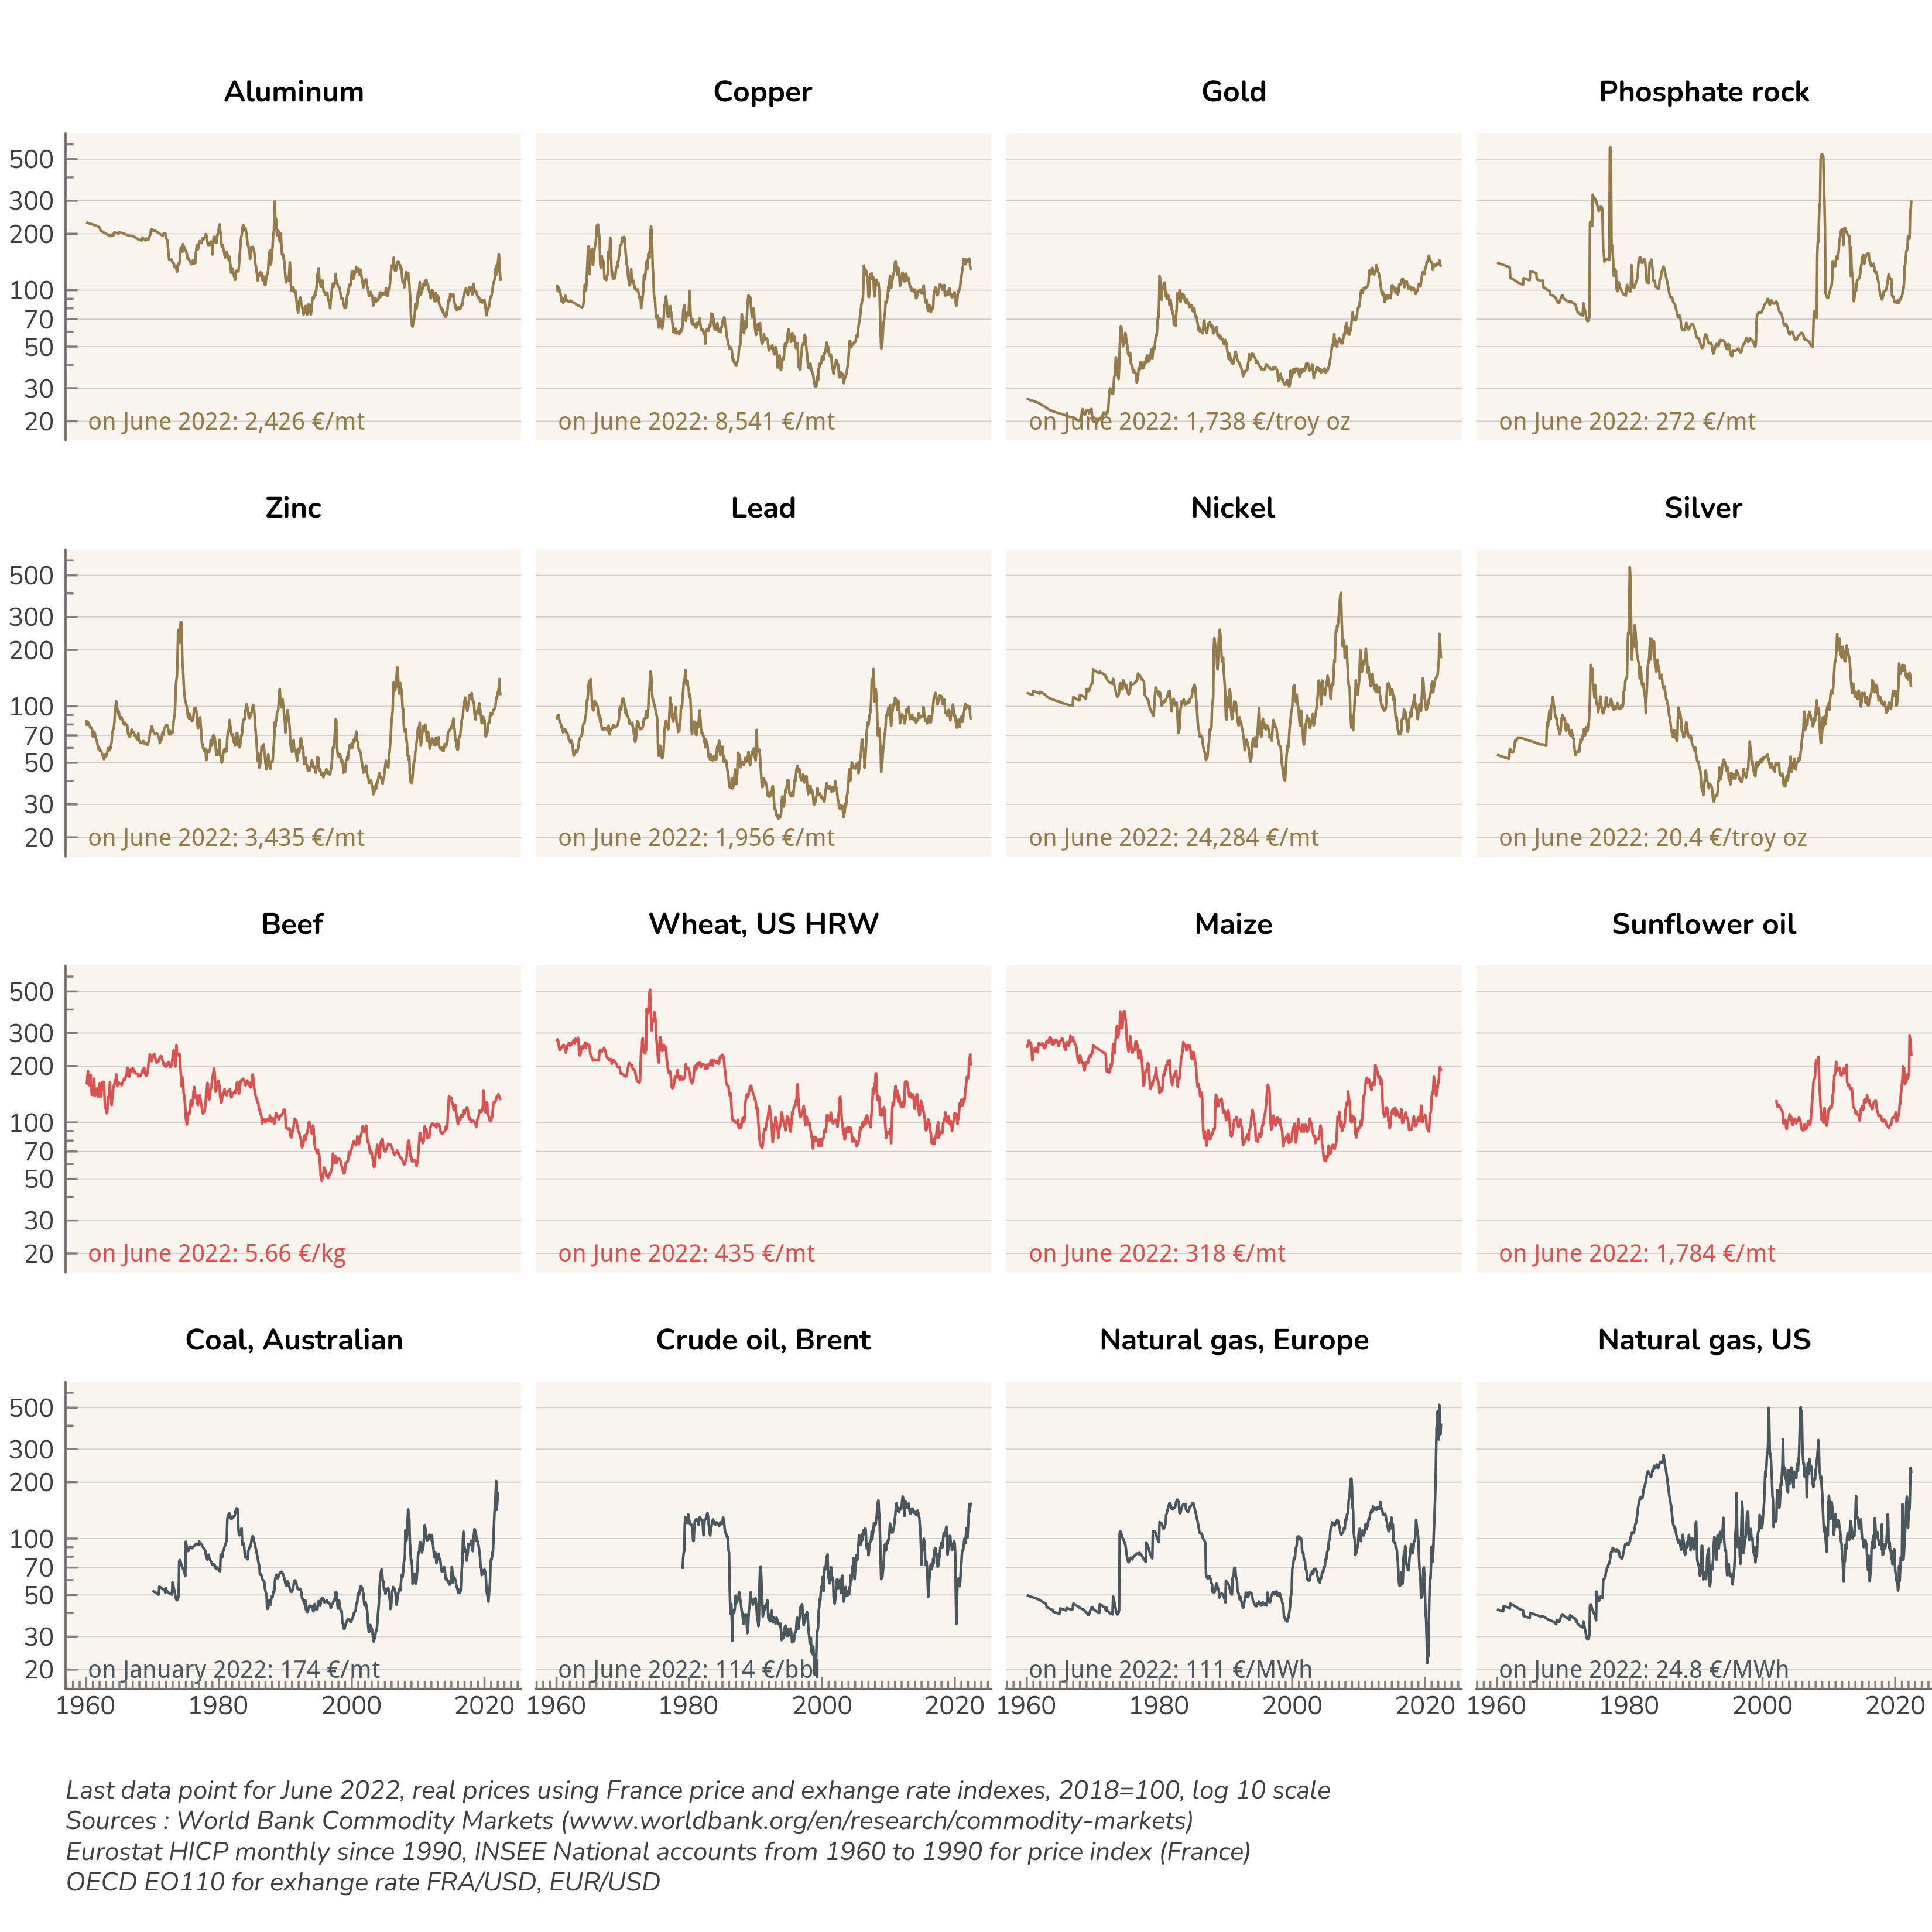
\includegraphics[width=1\textwidth,height=\textheight]{SIWU_brief_files/figure-pdf/fig-com-1.png}

}

\end{figure}

However, gas is not used in small islands like Cyprus and Malta (0\%);
and marginal in Sweden (0,3\%) and Finland (0,5\%), who use mostly
derived heat and electricity (see Figure~\ref{fig-nrg}). On the other
hand, gas represents the majority of energy in housing in the
Netherlands (69,3\%) and Italy (51,8\%). Also, the need of energy might
differ between nations, especially for heating purposes due to climate
and thermal efficiency of housings: households in Malta, Portugal, Spain
and Cyprus use far less energy than in Luxembourg, Austria and Denmark.
Likewise, passenger mobility differs between Italy, Norway, Finland,
Germany, France (above 13 000 km per capita per year) on one hand, and
Romania and Slovakia (around 7 500 km/c/y)\footnote{Odyssee-Mure:
  \url{https://www.odyssee-mure.eu/publications/efficiency-by-sector/transport/passenger-mobility-per-capita.html}}.
Moreover, only 30\% of travel distance in Romania is by car as driver
against 63\% in Italy. Some, but not all, of these differences can be
attributed to income differences.

Countries, gas and electricity companies and consumers are affected
differently in the European Union through volumes, but also through
prices. Despite price convergence due to the evolution towards
liberalisation and a single European energy market, national utilities
and consumers face different prices depending on the contracts signed
with suppliers.

\begin{figure}[htb]

\caption{\label{fig-nrg}Energy final consumption per capita by vector}

{\centering 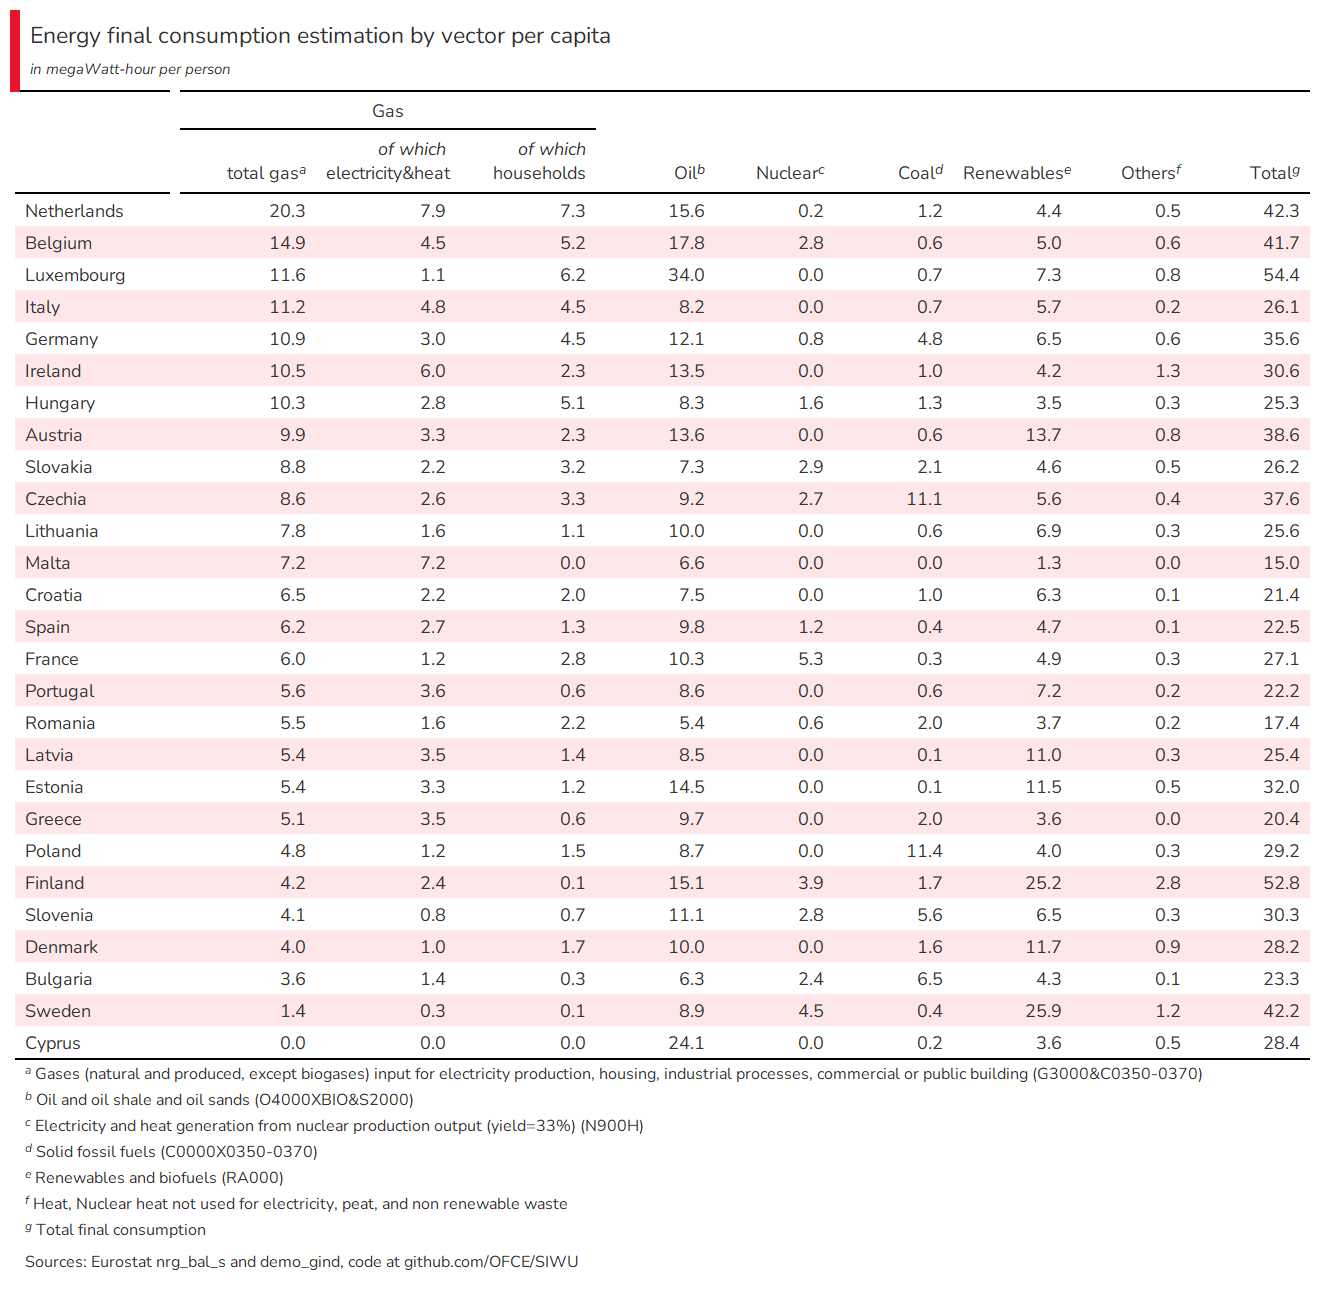
\includegraphics[width=1\textwidth,height=\textheight]{../svg/tab1.png}

}

\end{figure}

Most European countries have gone from oil-indexation to gas-indexation
in the long-term contracts signed with gas suppliers. In the European
Union, oil-indexation represented nearly 80\% of contracts in 2005, and
only around 20\% in 2019, replaced by gas-indexation. This trend
started, and is most pregnant in Northwest Europe (Belgium, Denmark,
France, Germany, Ireland, Luxembourg, Netherlands). The change is less
dramatic in Mediterranean (Greece, Italy, Portugal, Spain). Gas-indexed
contracts have not really increased in South-east Europe (Bulgaria,
Croatia, Romania) or Scandinavia and Baltics (Finland, Sweden,
Lithuania, Latvia, Estonia). This is important because, in this crisis,
oil has not increased as much as gas (Brent is up 52\% in 1-year, 35\%
year-to-date). Also, consumers might be more or less protected by the
contracts they signed with the gas and electricity utilities. There is a
trend towards more variable-price contracts, especially in countries
like Luxembourg, Slovenia, Ireland, Spain, Belgium, Czech Republic and
the Netherlands: in these countries, more than 50\% of consumers have
variable-pricing gas contracts. In Belgium, suppliers have the right to
index their variable gas and electricity prices monthly and use the
indexing parameters of their choice (of course, they might wish to link
it directly to their wholesale price so that they do not take any market
risk). The government justified the decision in the objective to ``bring
the bill closer to the market reality''. However, if demand is
relatively inelastic in the short-term, this price-liberalisation
increases volatility and risk for countries that produce gas as well as,
and more importantly in this case, final consumers.

Consequently, the impact on consumers, as analysed in this study, does
not presume of the impact on the economy as a whole: the cost of the
price increase can also be borne by the state (through subsidies), or by
state or private utilities tied by regulations (in France, EDF bore part
of the total cost of electricity price increases). Impact on households
might differ according to the preferred policy response: freeze in
prices compensated by corporate subsidies or direct transfers to
vulnerable households according to income and/or energy consumption. In
both cases, computability will be different: in the first case, for the
same amount of additional government deficit, there will be no or less
change in prices and income, whereas in the second case both prices and
household income will soar.

We can distinguish several kind of policies that have a different impact
on what we measure in this report:

\begin{itemize}
\item
  What most economists would suggest in normal times is to not touch the
  `price-signal' and compensate the poorest households with energy
  cheques. This would not impact the inflation as measured in this
  report but the decrease in living standard is partially compensated,
  borne by the state, depending on generosity of the cheque.
\item
  One can also stress that the impact on welfare of energy price
  increases depends both on income and energy needs. Governments can
  therefore compensate consumers via cheques that also depend both on
  income and energy consumption in the last months. This does not
  decrease the price of energy (which would increase demand) but
  compensate according to volumes consumed. With such a strategy,
  inflation could remain high, but compensated by the State according to
  historical consumption: there would probably less winners and losers
  (i.e.~variations in living standard) than with a compensation based
  solely on income.
\item
  Alternatively, governments can act to deflate prices via (temporary)
  tax cuts or direct subsidies, and/or price caps, for all or for the
  most vulnerable in income and/or energy needs. Price subsidies for all
  is the most expensive instrument for the state budget, and it
  increases demand (relatively to other policies) for energy. It is not
  usually recommended by economists who think in terms of cost/benefits
  analysis. However, if everyone is preserved from price increases in
  the short term, it prevents the crisis from becoming a political
  issue: the truen b cost and transfers are hidden, or a least their
  discussion is temporarily transferred to, it is hoped, after the
  crisis (when the true aggregate cost is supposedly known and political
  discussion does not depend on anticipations).
\end{itemize}

This later element has some consequences for monetary policy. By cut
price increase before they reach consumer price, ones prevent indexation
mechanism (pension, minimum wage, social compensation) and thus prevents
partly so called second turn effects. This then simplify the conduct of
the monetary policy as response to external price shocks can't be
countered by a restrictive monetary policy. Thus by preventing partially
pass through to the economy, at a high fiscal cost, monetary policy can
be free of inflation risk and address the slowdown of the economy
induced by the transfer to commodities producers.

\hypertarget{results-general-discussion}{%
\section{Results: general discussion}\label{results-general-discussion}}

The 3 following graphs
(Figure~\ref{fig-priceinc1}, Figure~\ref{fig-priceinc2}, Figure~\ref{fig-priceinc3})
are displaying the most important increases in prices since the
beginning of the war in Ukraine.

In most countries, the COICOP categories concerned by prices increases
are transportation especially CP0722 which are ``Fuels and lubricants
for personal transport equipment'', and various categories of energy for
housing (heating, hot water or appliances), in the categories CP0451 to
CP0454 (Electricity, Gas, liquid fuel, solid fuel). In some countries,
some food categories are displaying a sharp increase (especially oils
and fat). Annex tables are summarizing the most important increases.

\begin{figure}[htb]

\caption{\label{fig-priceinc1}Price increase since War in Ukraine (1/3)}

{\centering 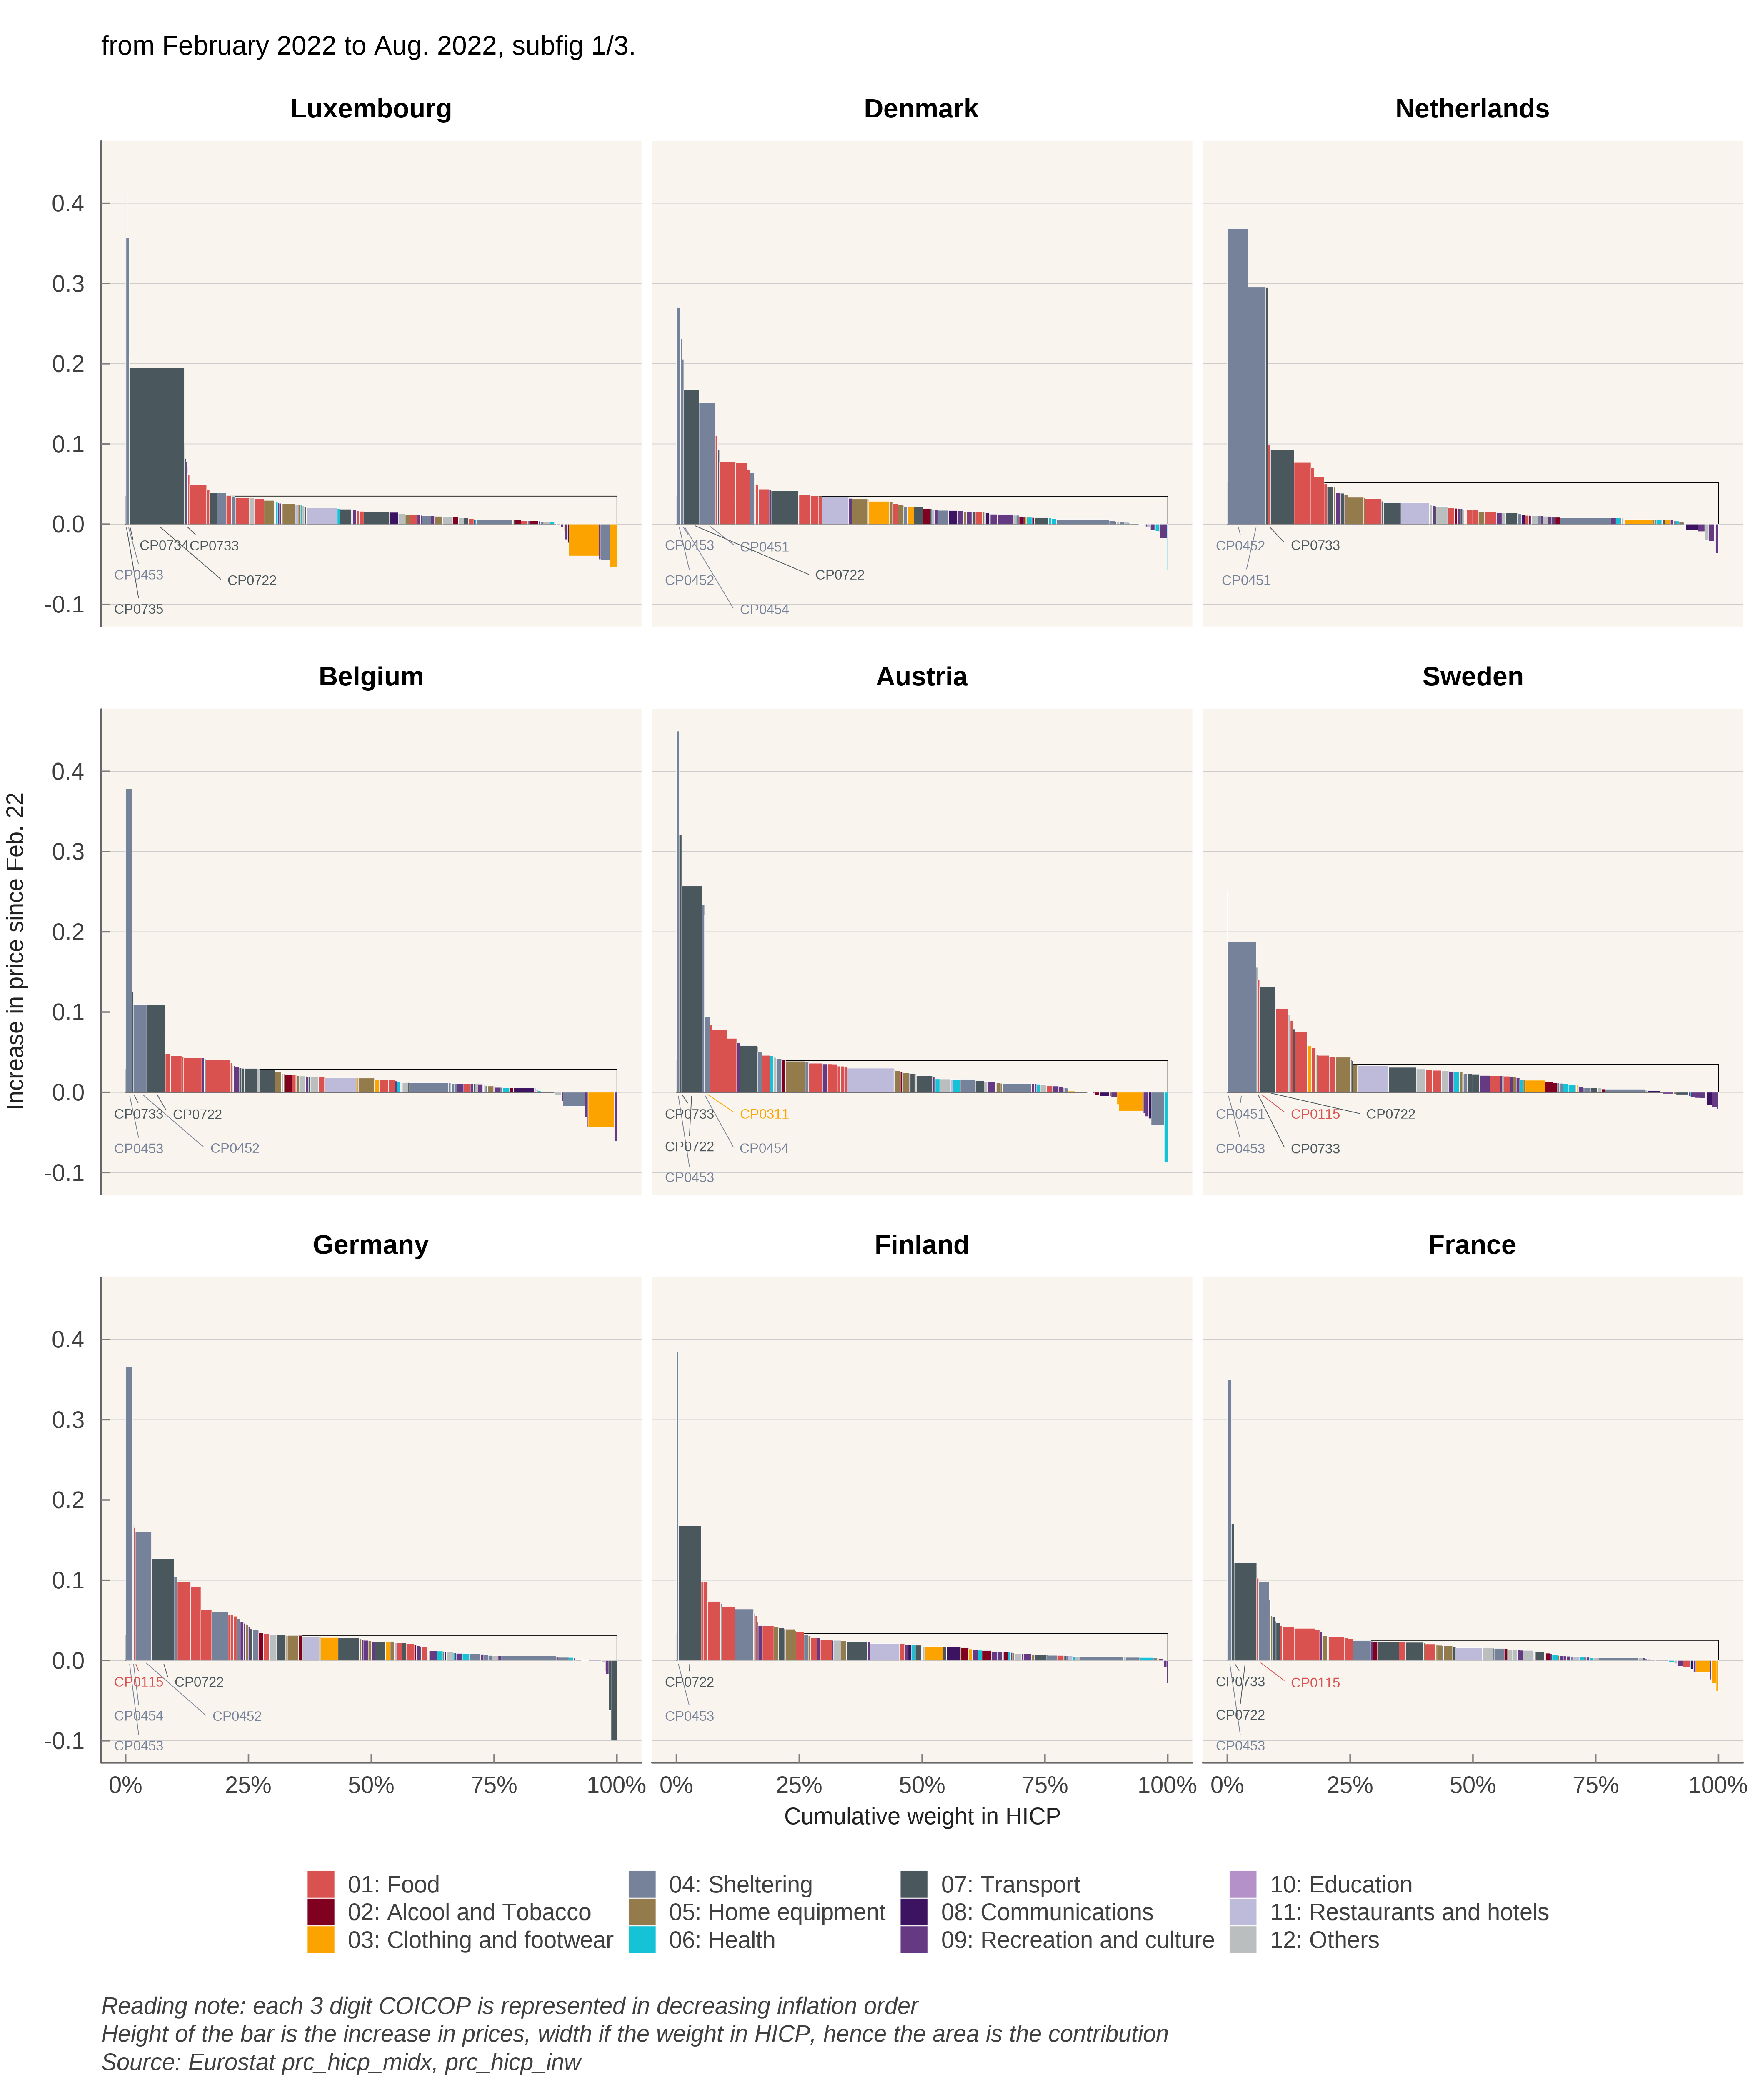
\includegraphics[width=1\textwidth,height=\textheight]{SIWU_brief_files/figure-pdf/fig-priceinc1-1.png}

}

\end{figure}

\begin{figure}[htb]

\caption{\label{fig-priceinc2}Price increase since War in Ukraine (2/3)}

{\centering 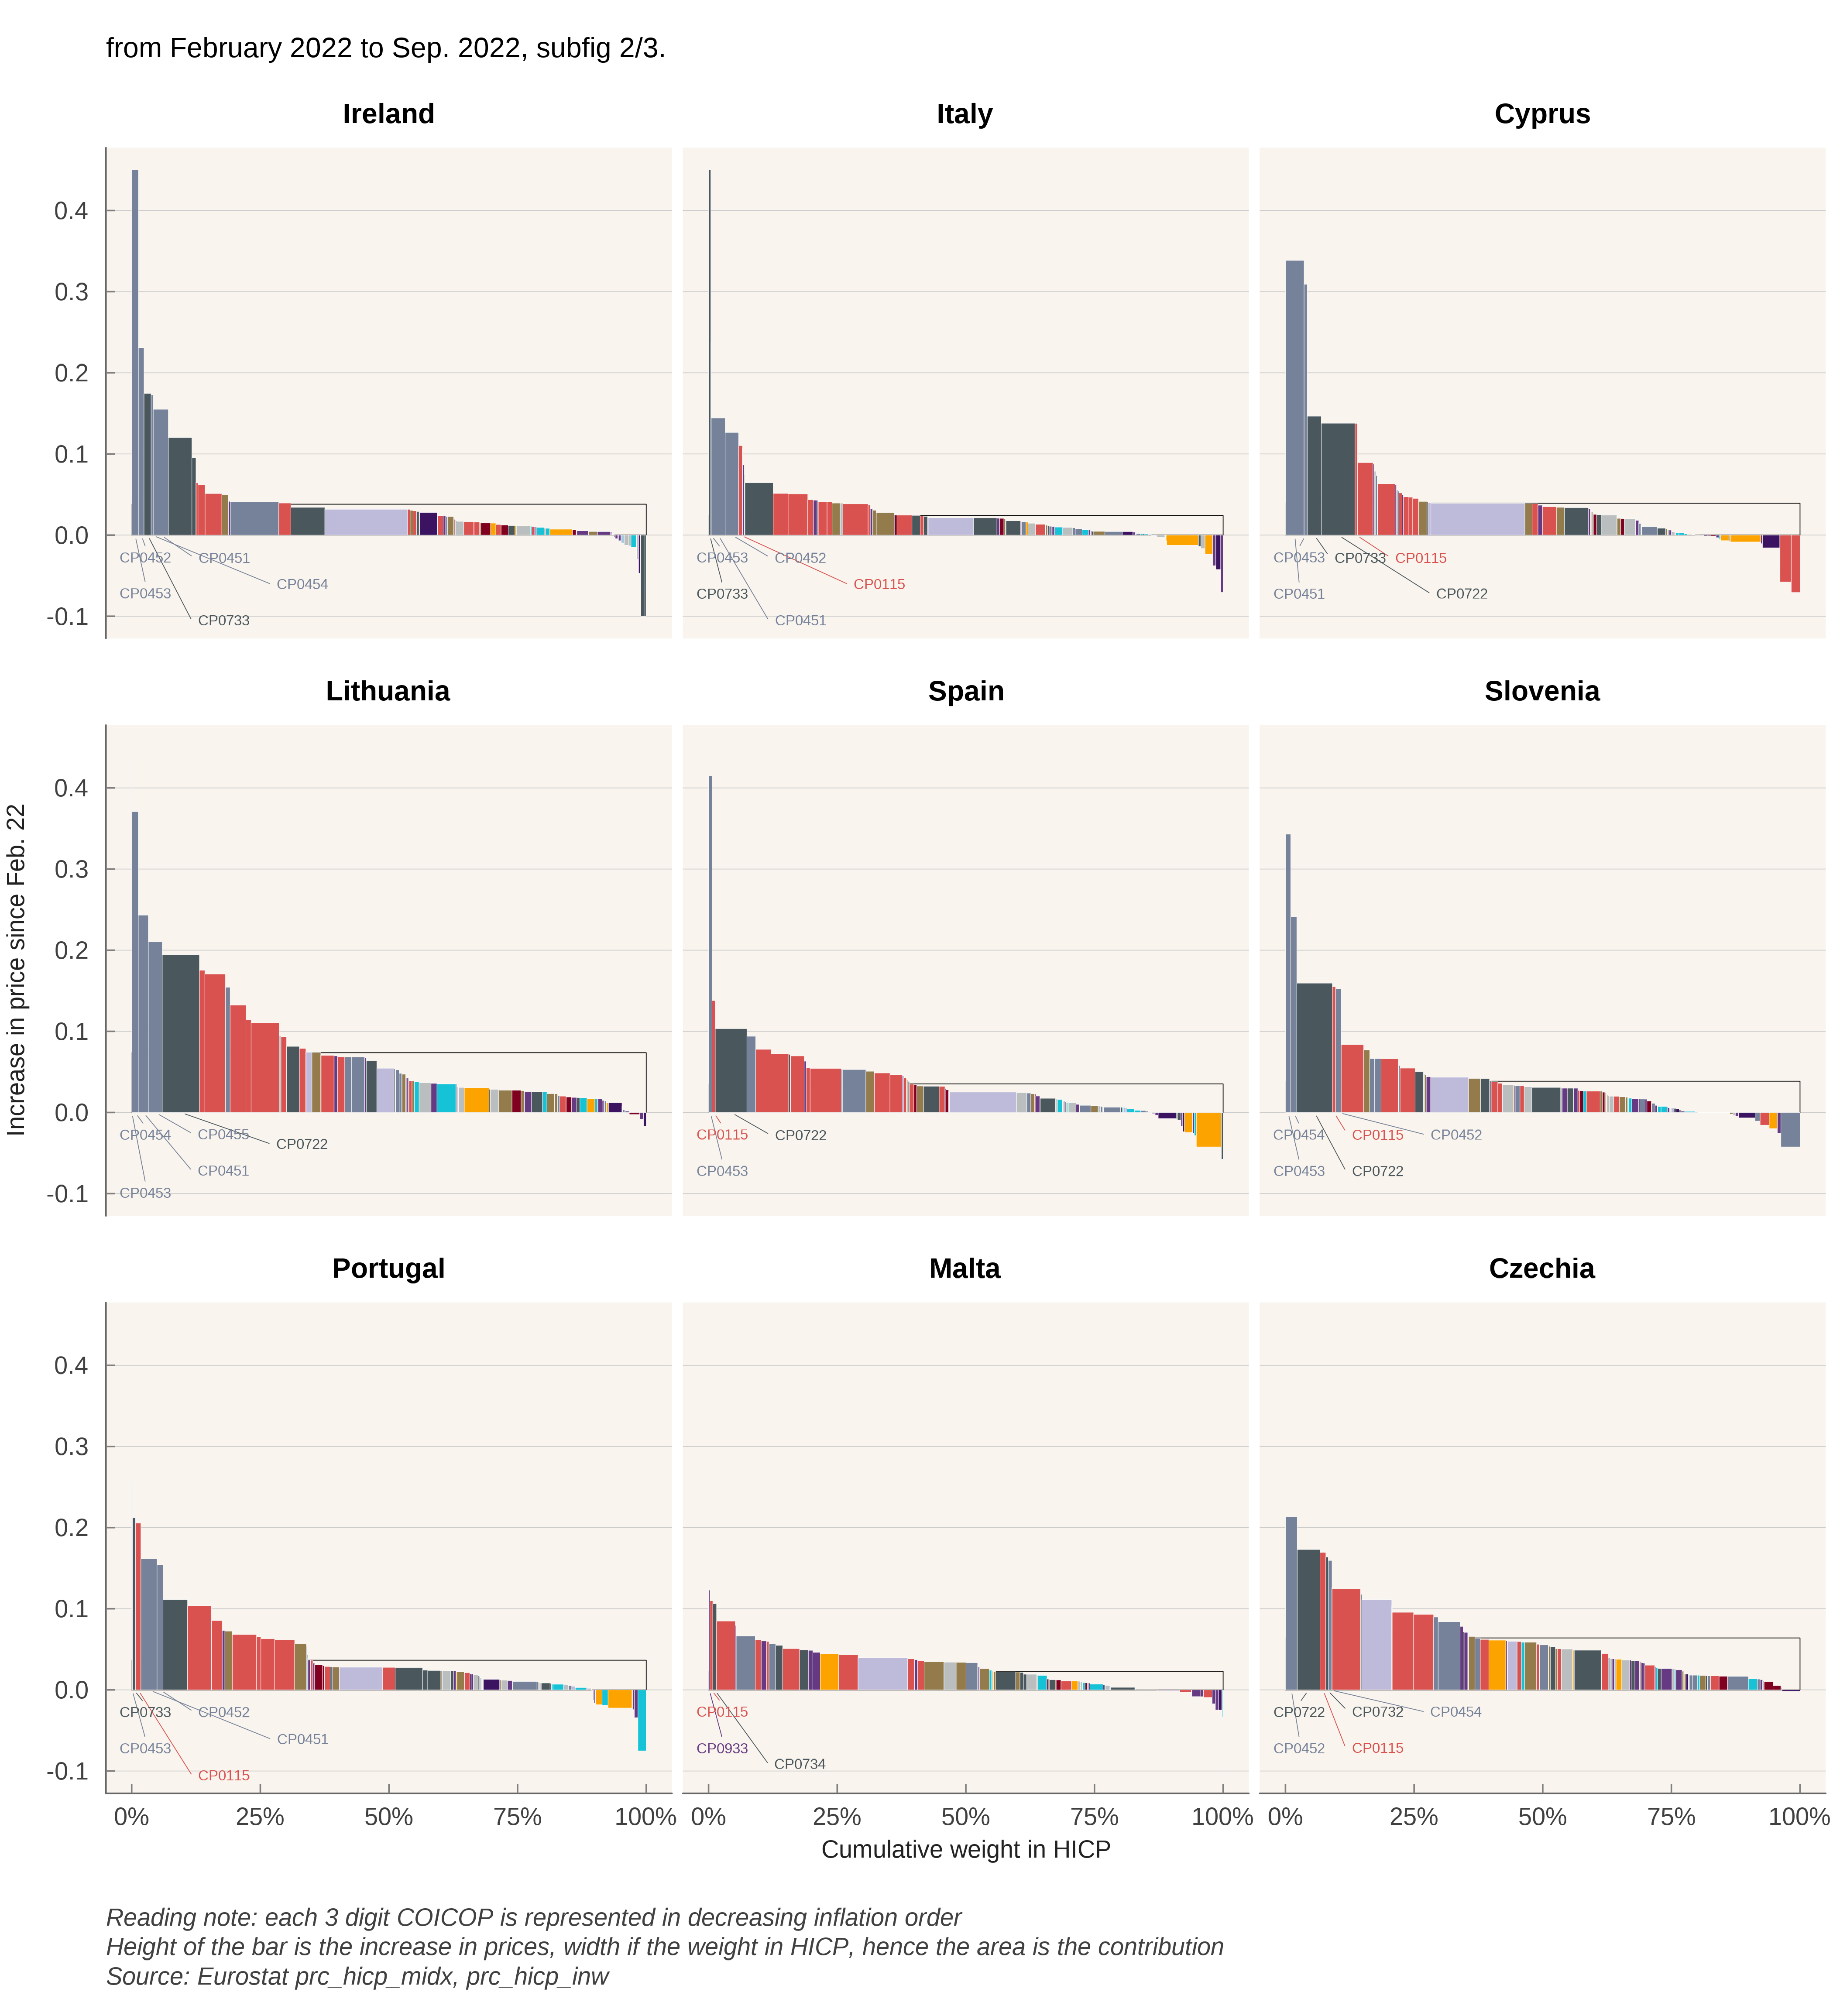
\includegraphics[width=1\textwidth,height=\textheight]{SIWU_brief_files/figure-pdf/fig-priceinc2-1.png}

}

\end{figure}

\begin{figure}[htb]

\caption{\label{fig-priceinc3}Price increase since War in Ukraine (3/3)}

{\centering 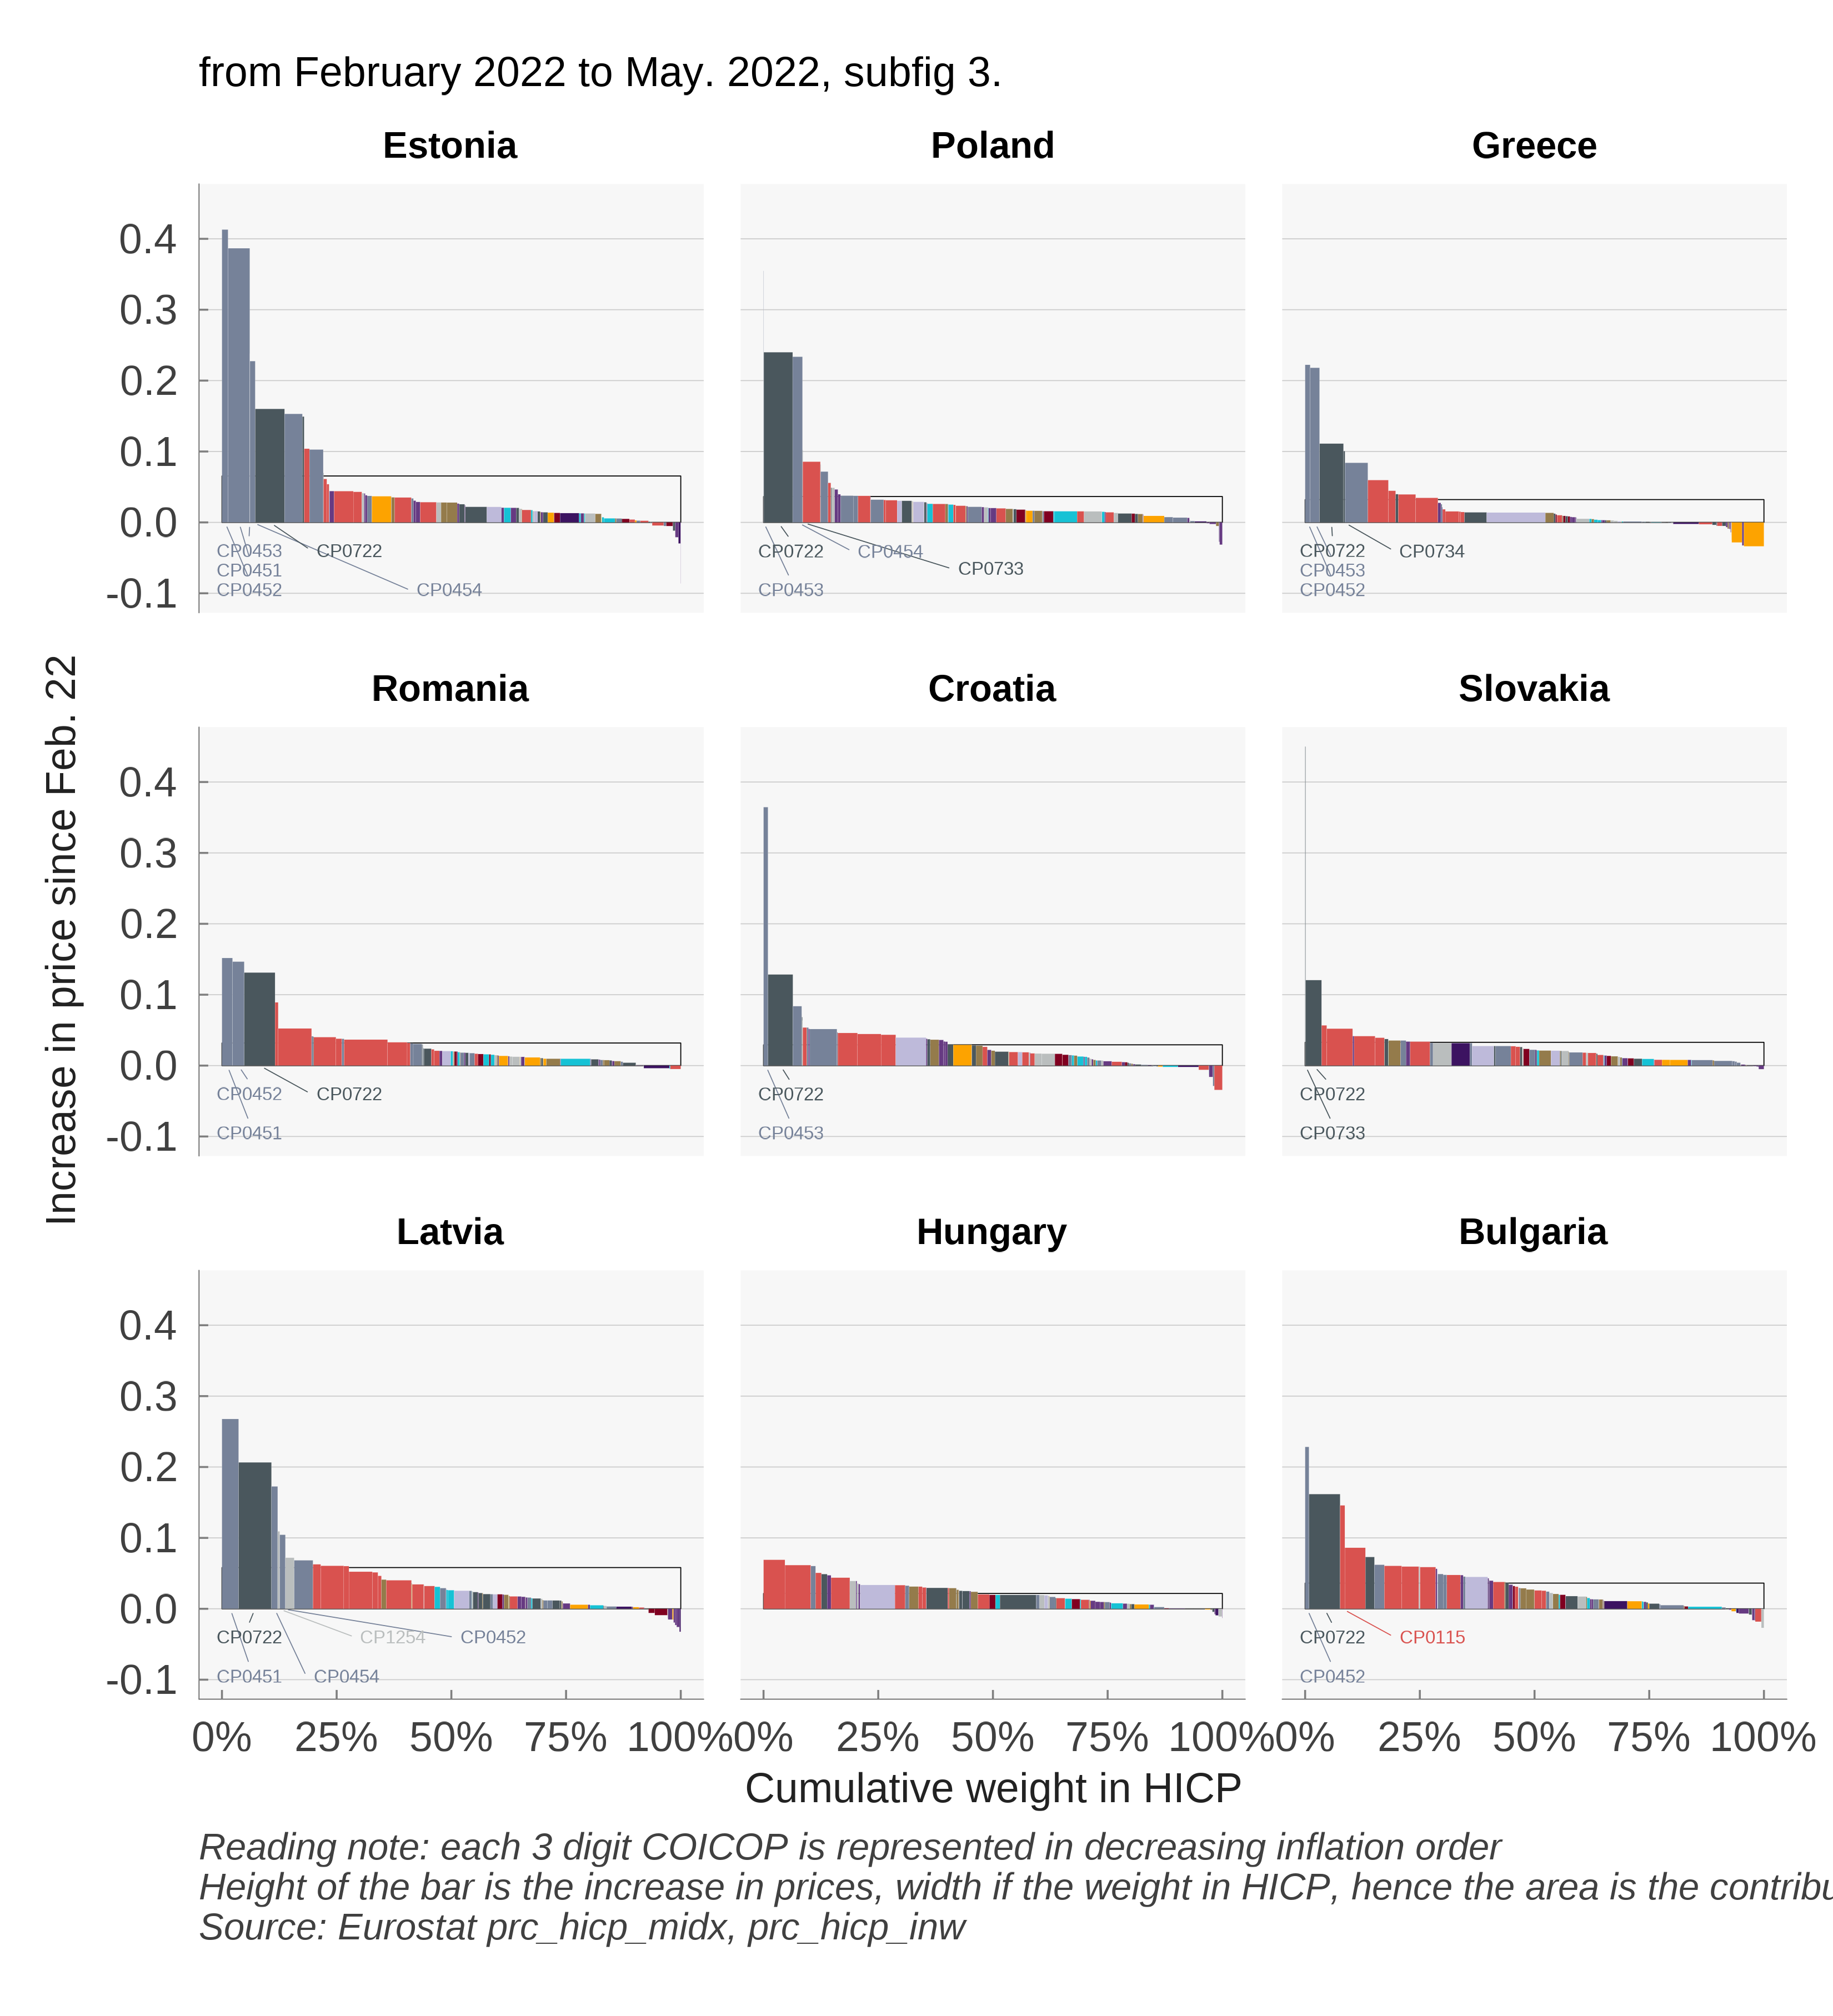
\includegraphics[width=1\textwidth,height=\textheight]{SIWU_brief_files/figure-pdf/fig-priceinc3-1.png}

}

\end{figure}

\FloatBarrier

The following 3 graphs (see Figure~\ref{fig-impact1},
Figure~\ref{fig-impact2}, Figure~\ref{fig-impact3}) are displaying the
breakdown by quintile of the impact in purchasing power per countries.

\begin{figure}[htb]

\caption{\label{fig-impact1}Impact on income per quintile (1/3)}

{\centering 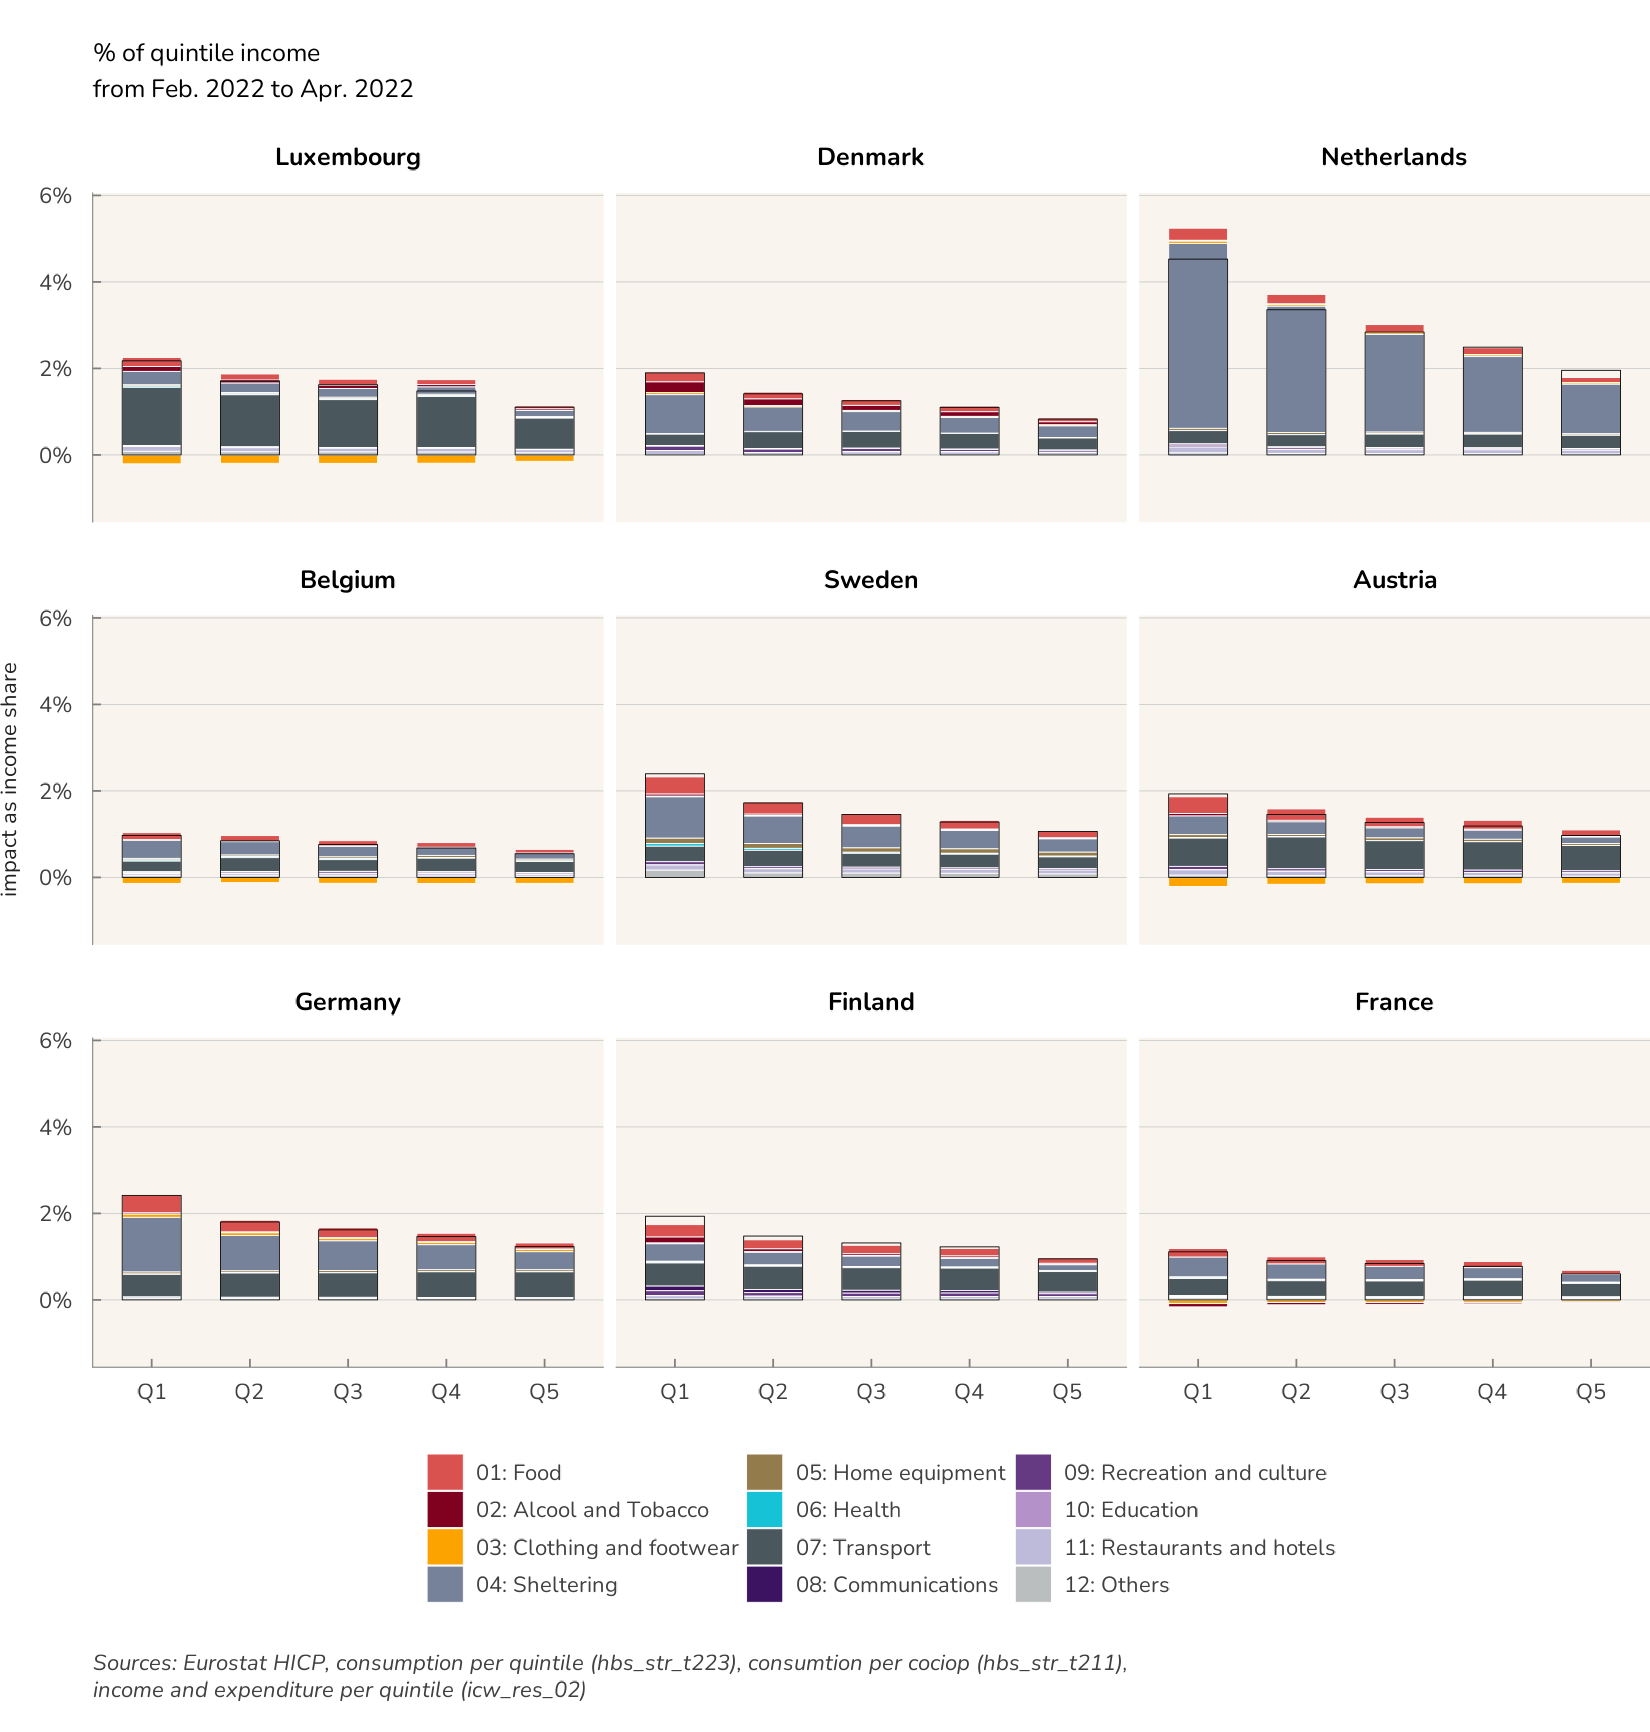
\includegraphics[width=1\textwidth,height=\textheight]{SIWU_brief_files/figure-pdf/fig-impact1-1.png}

}

\end{figure}

\begin{figure}[htb]

\caption{\label{fig-impact2}Impact on income per quintile (2/3)}

{\centering 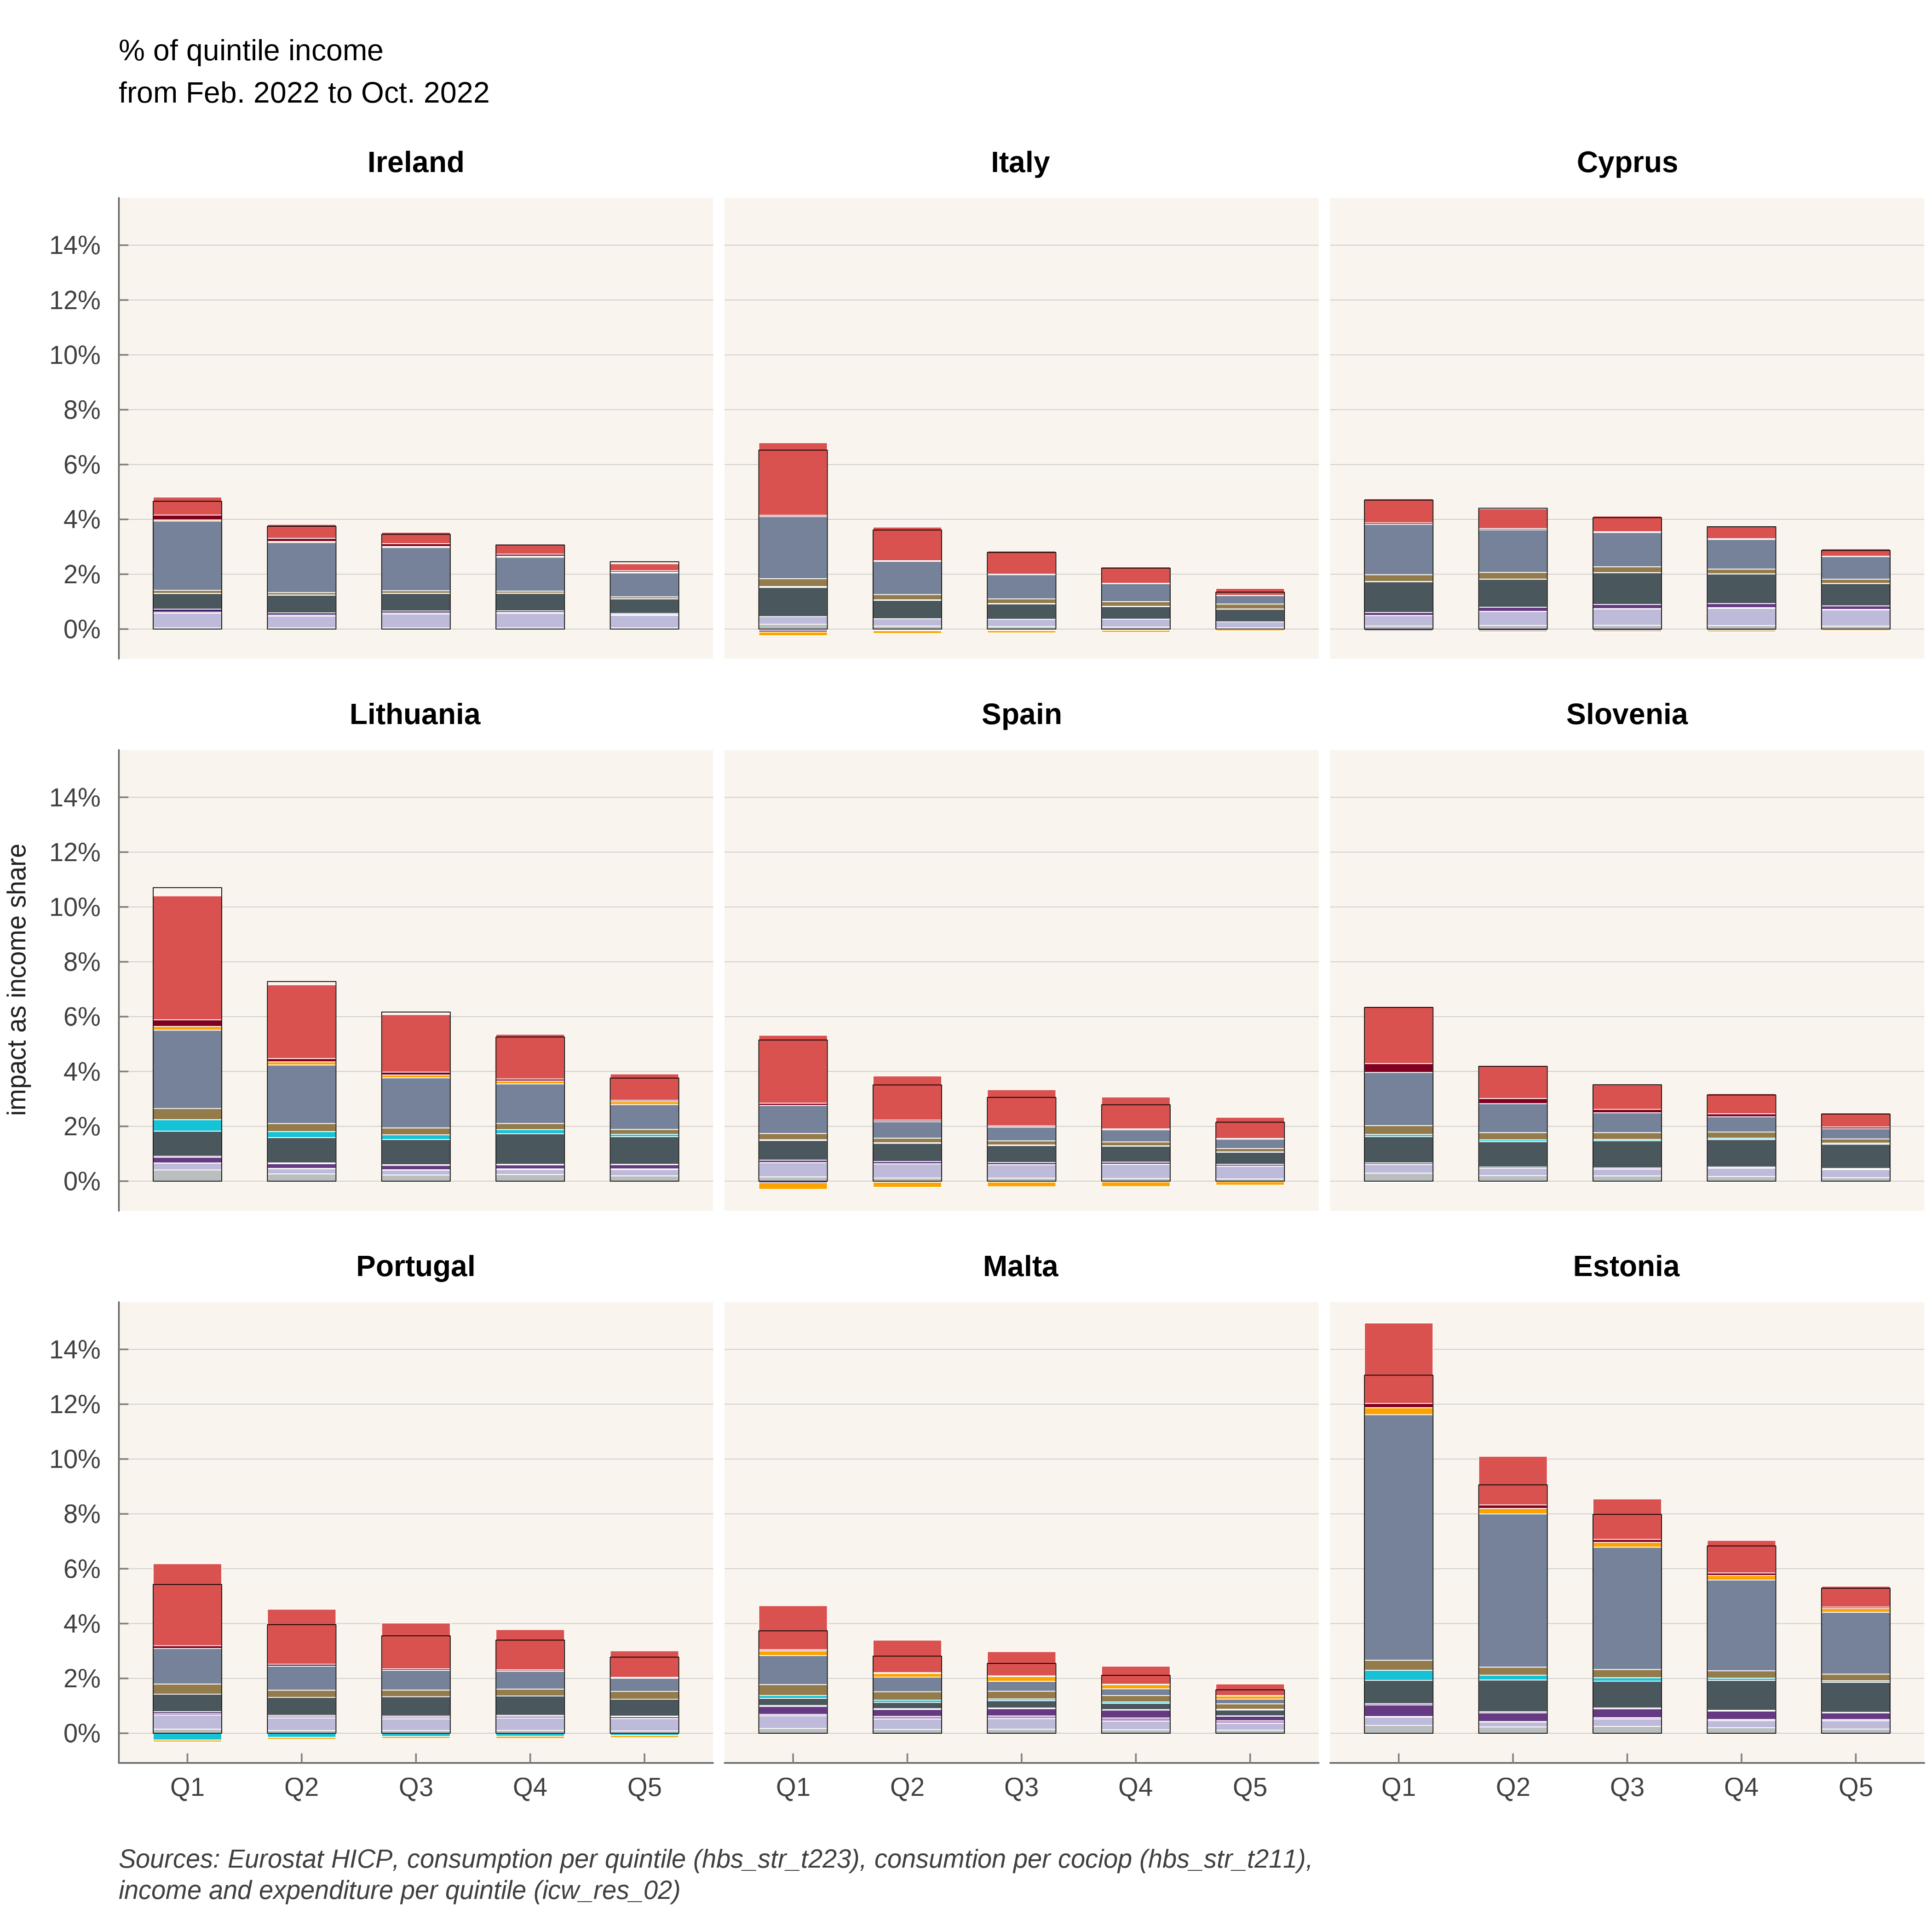
\includegraphics[width=1\textwidth,height=\textheight]{SIWU_brief_files/figure-pdf/fig-impact2-1.png}

}

\end{figure}

\begin{figure}[htb]

\caption{\label{fig-impact3}Impact on income per quintile (2/3)}

{\centering 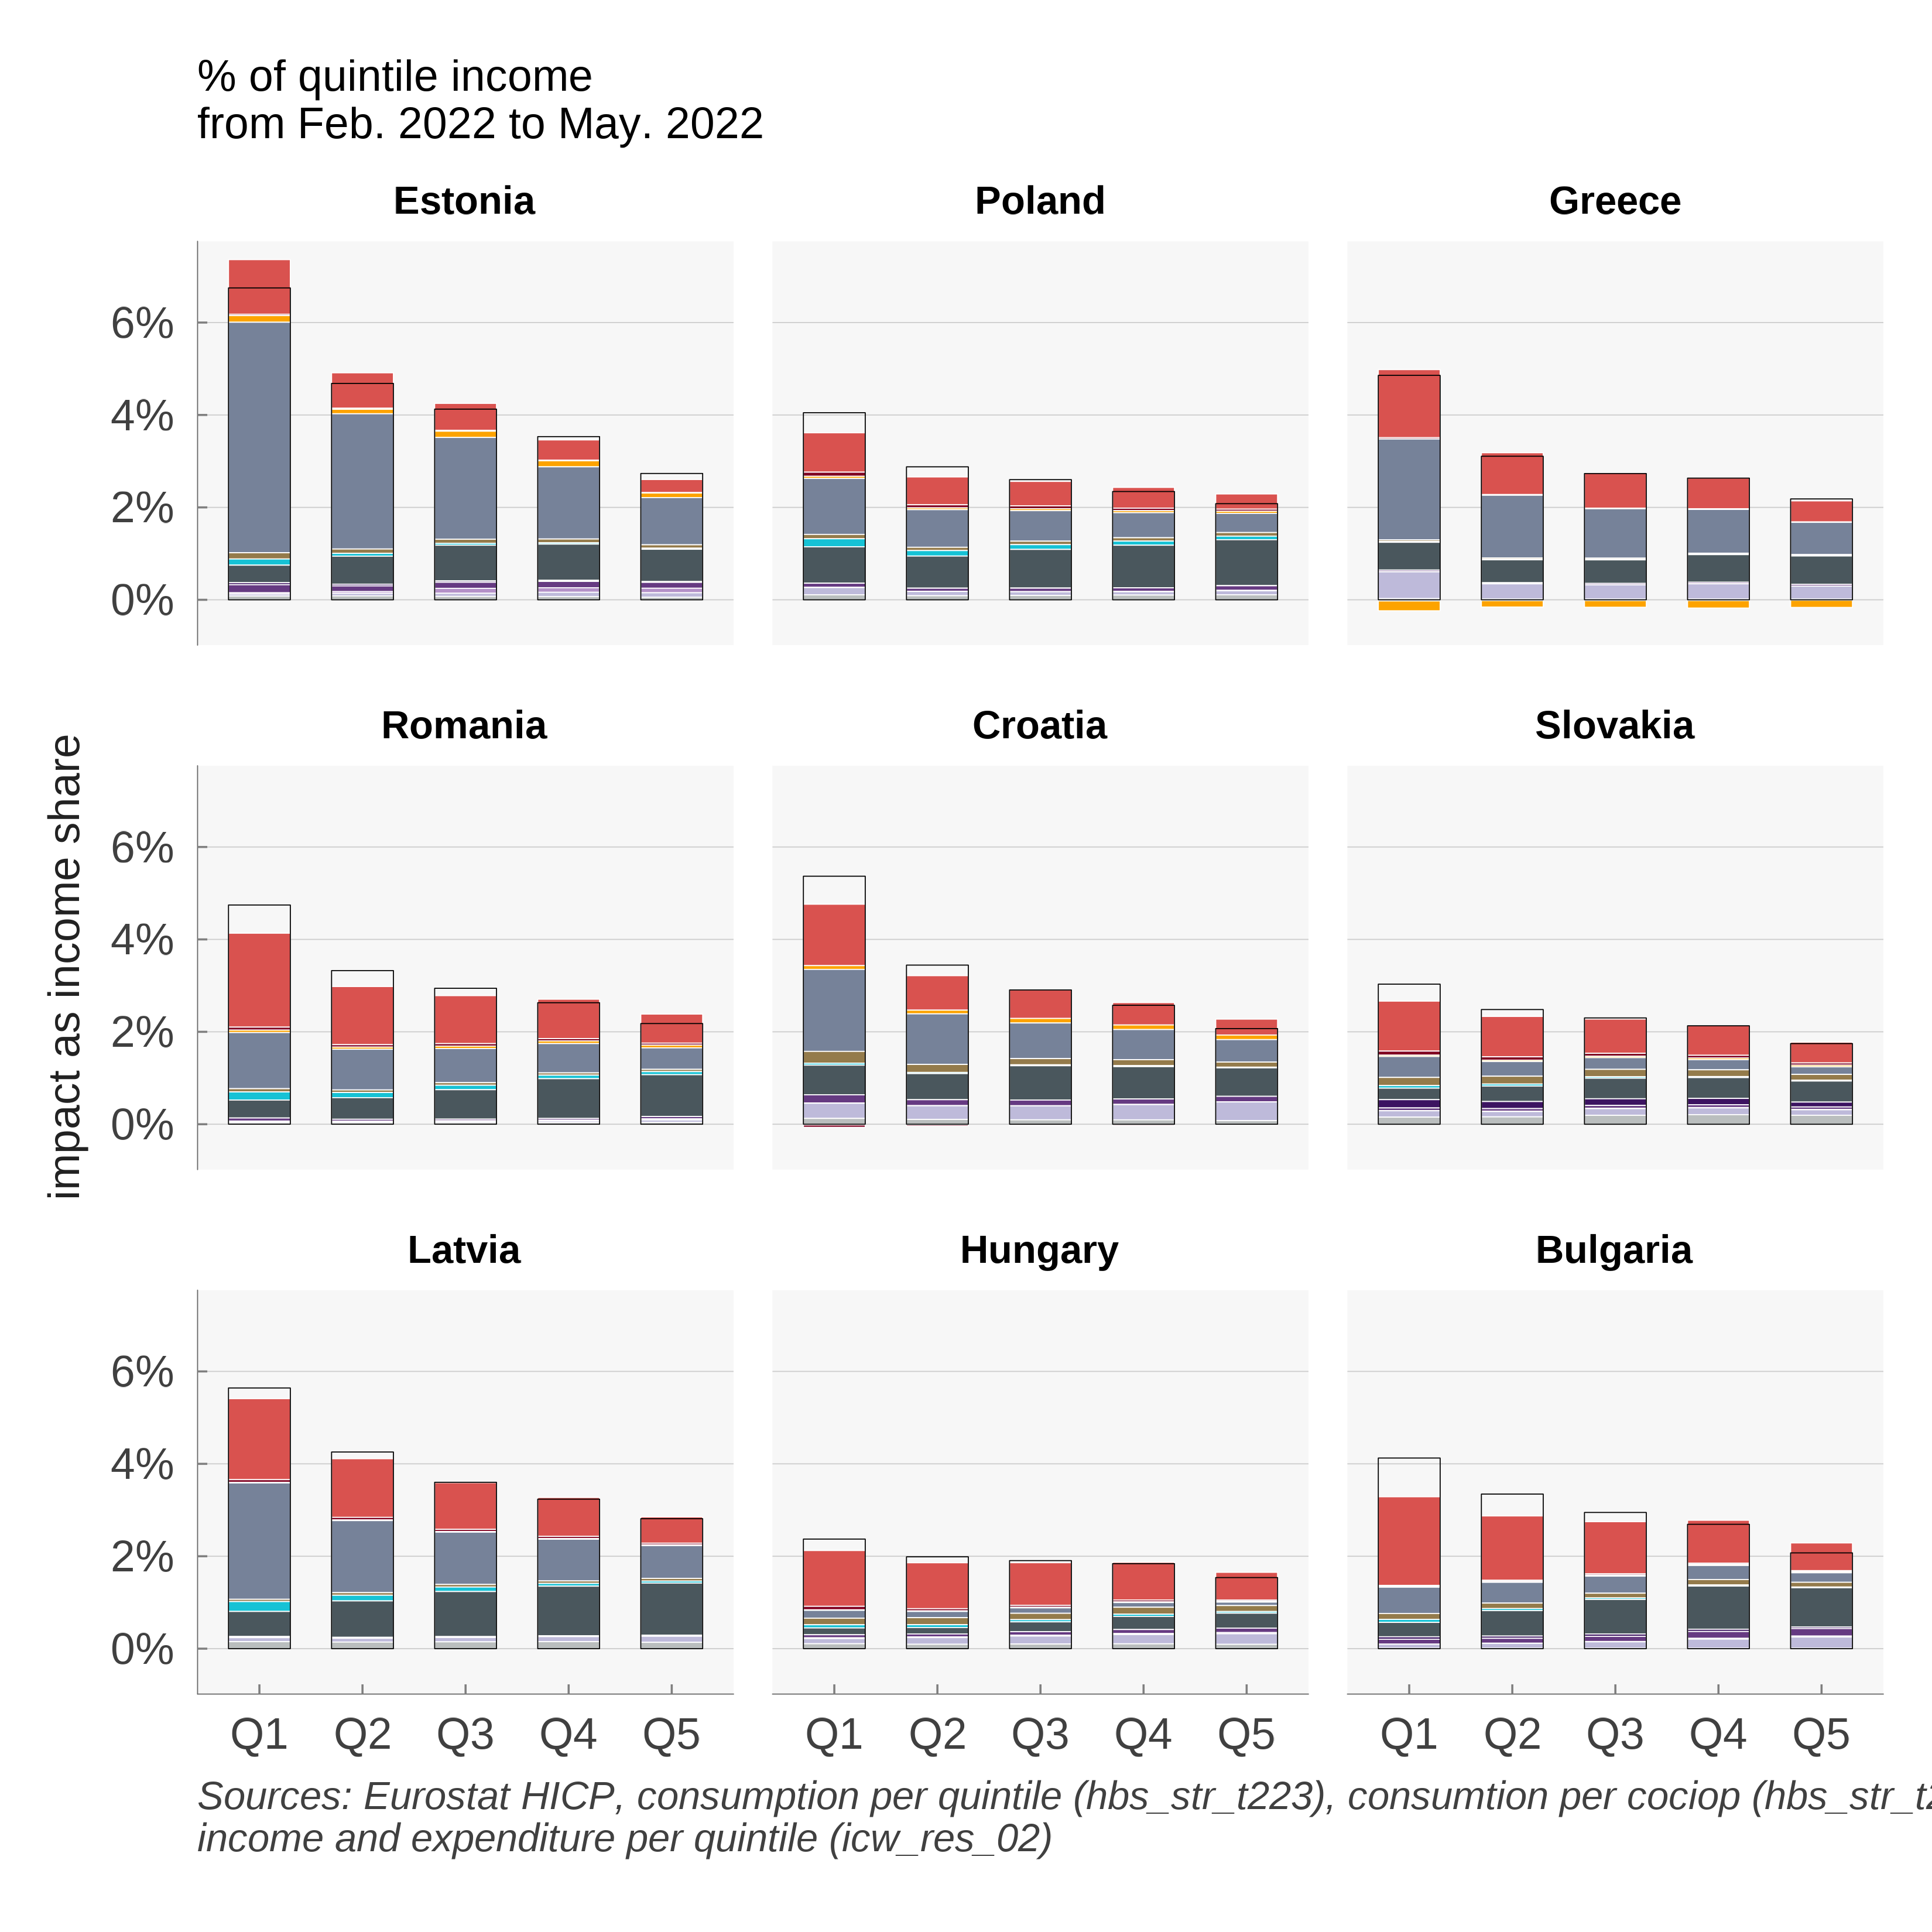
\includegraphics[width=1\textwidth,height=\textheight]{SIWU_brief_files/figure-pdf/fig-impact3-1.png}

}

\end{figure}

\FloatBarrier

Compared to other countries, and due to governmental policies,
households in France are relatively preserved by price increases. This
is also the case in Sweden, Cyprus and Malta, three countries that are
not dependent on gas for household heating. In Sweden, use of gas or oil
for heating is marginal since 2010 for domestic heating. Oil, which
represented 50\% of energy consumption in the early 1980s has been
replaced by heat networks (that themselves rely only marginally on
fossil fuel)\footnote{According to Swedish Environmental Agency, total
  greenhouse gas emission from buildings (heating) decreased from 9.30
  million tonnes of carbon dioxide equivalents in 1990 to 0.9 in 2018
  \url{https://ec.europa.eu/energy/sites/ener/files/documents/se_2020_ltrs_official_translation.pdf}}
and electricity, also decarbonized. National differences in how
household are impacted today are therefore partly the consequence of
long-term policies (environmental and/or geopolitical).

On the contrary, households in the Netherlands and Belgium, who rely
mostly on gas for heating, are most affected. In Slovenia, price hikes
in housing are more than compensated by governmental measures (notably,
an exemption that decreased electricity prices by 35\% on average from
February to April). It is also noticeable that households in the first
income quintile tend to be more affected (before eventual governmental
transfers), in percentage of income. This is not surprising: poorer
households tend to consume more energy and food as a share of income.
Poorer households, from the first quintile, are most hit in Greece, the
Netherlands, Lithuania. This is due mostly to housing expenses in the
Netherlands, but food also plays a role in Greece and Lithuania. The
next Figure confirms this conclusion. We can clearly see that for all
countries (except Slovenia), the impact on households from the first
quintile (Q1) is greater than for the richest households (Q5). This is
particularly true in Lithuania, the Netherlands and Greece. The
difference between Q5 and Q1 is also greater in countries where
households are most affected: the poorest households bear the most risk
from energy and food price volatility.

\begin{figure}

\caption{Impact on quintile}

{\centering 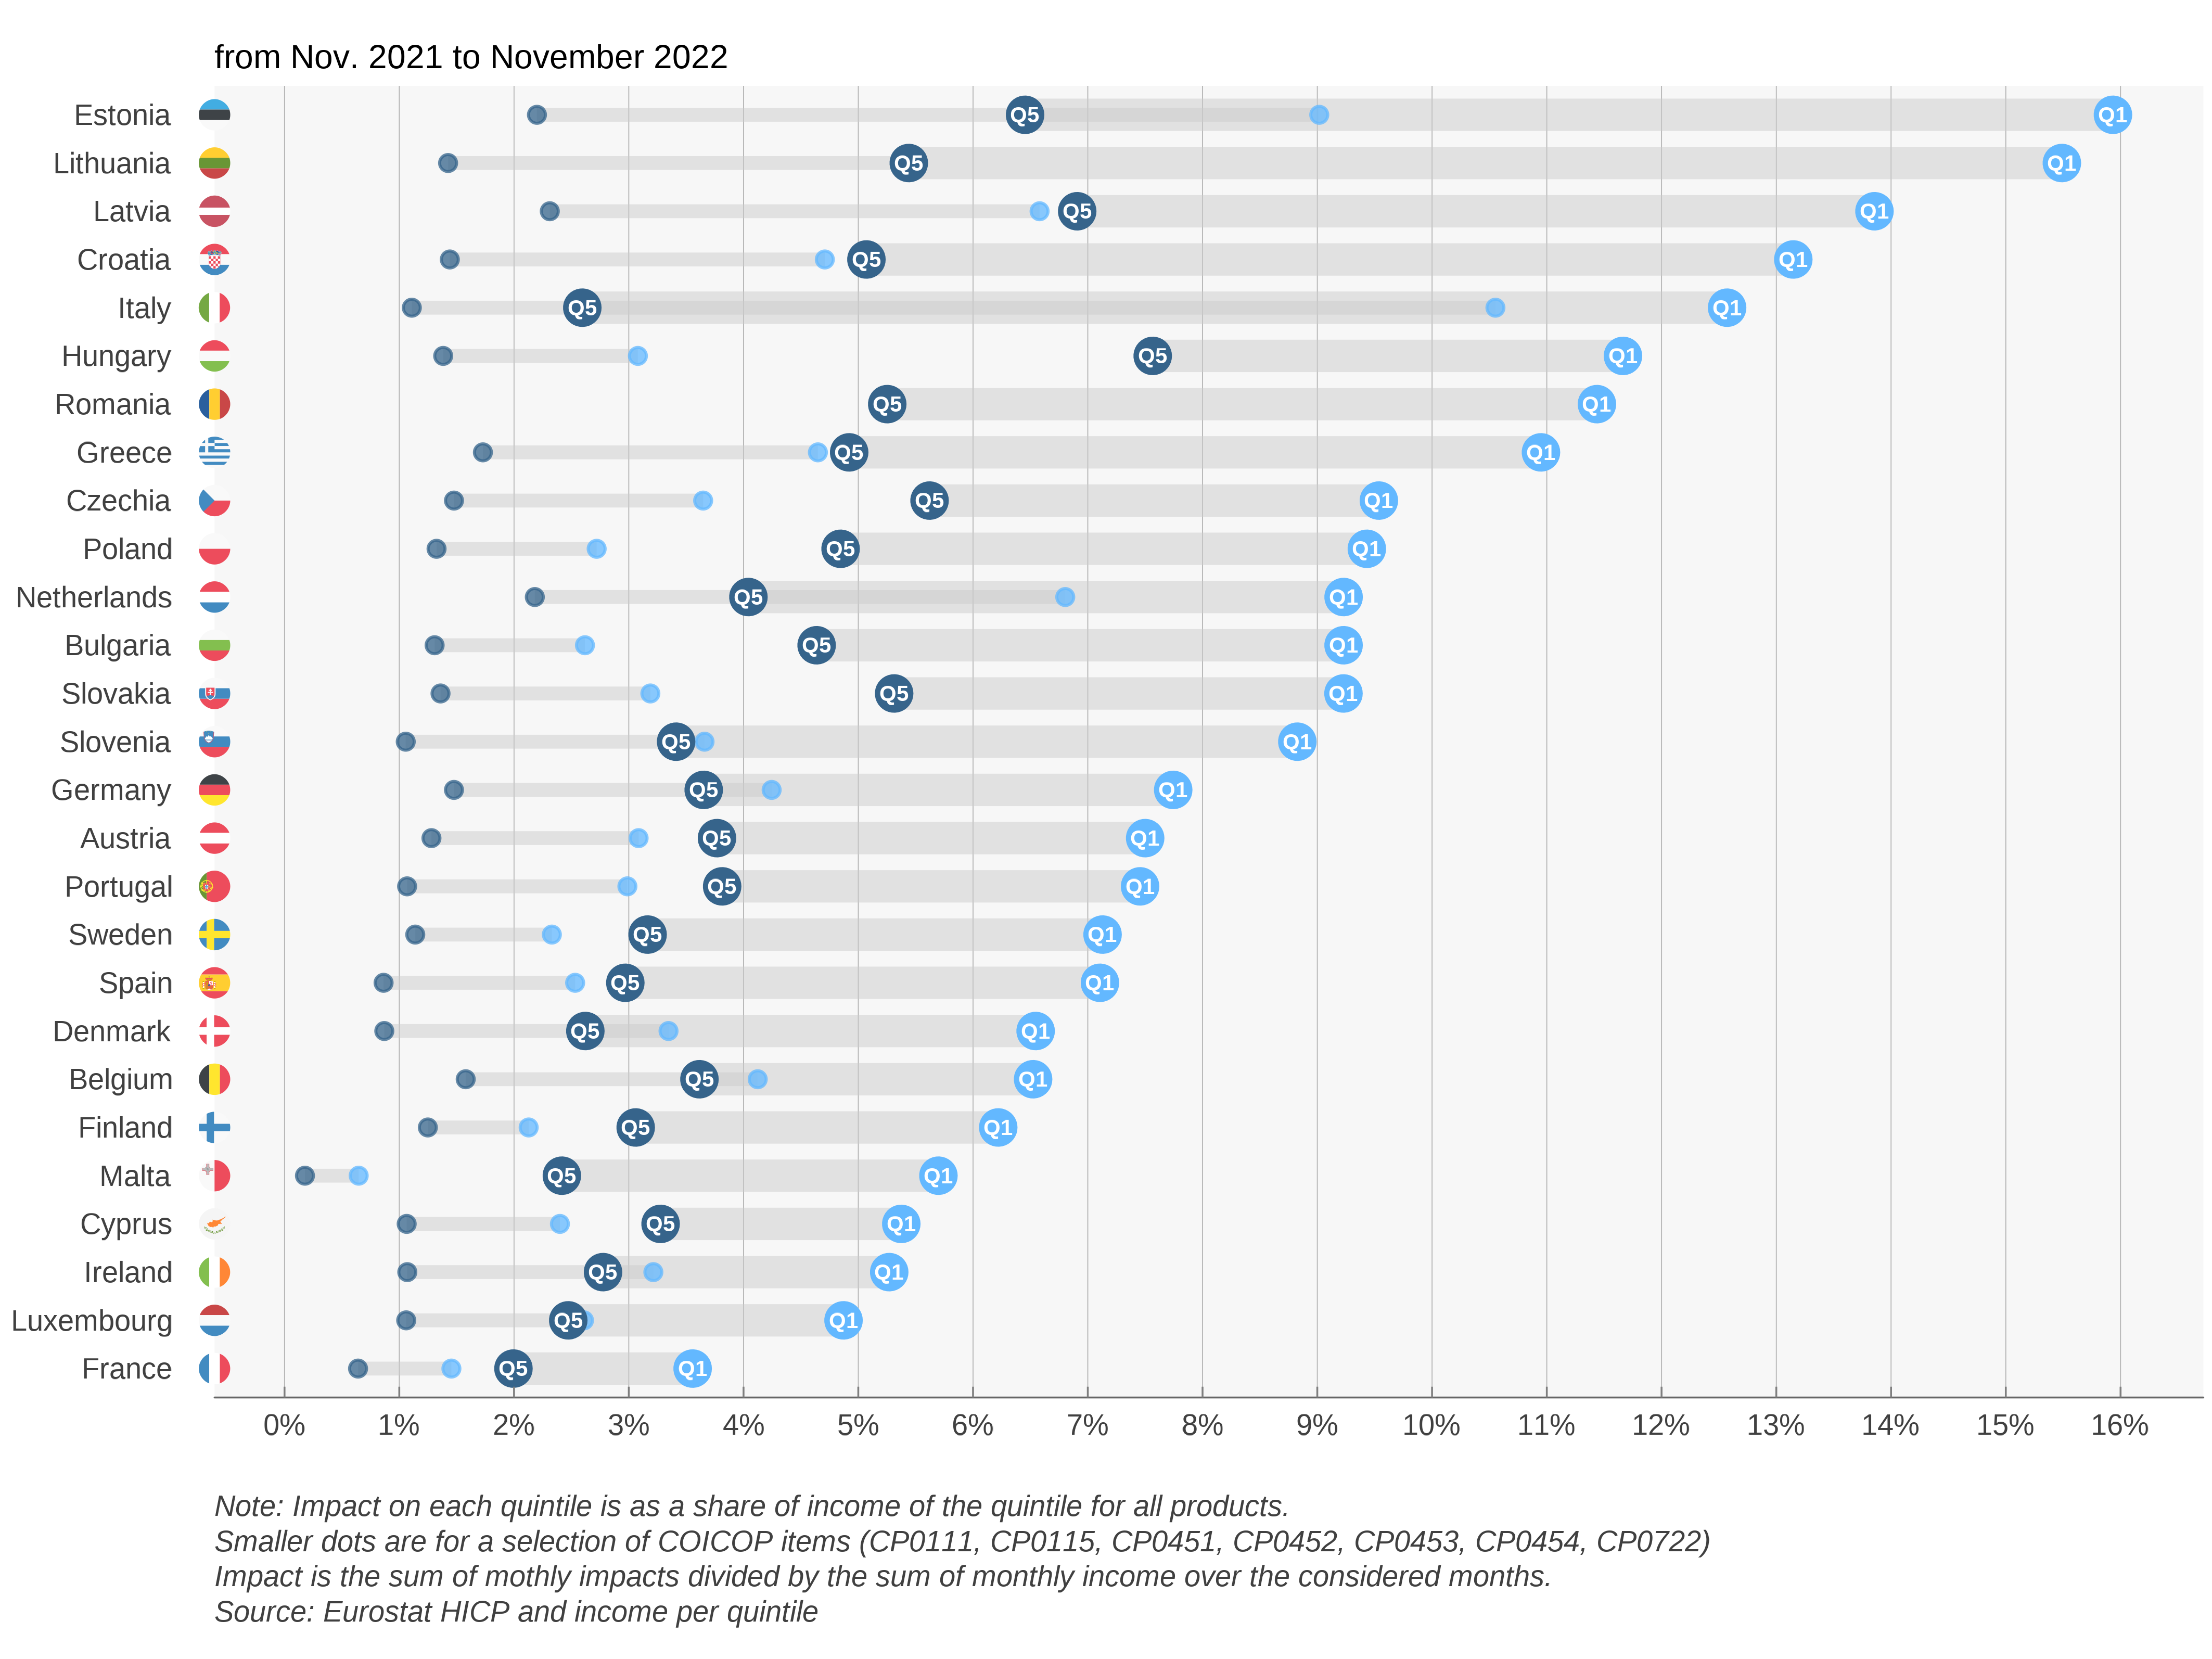
\includegraphics{../svg/quantiles1et5.png}

}

\end{figure}

\FloatBarrier

\begin{tcolorbox}[enhanced jigsaw, toprule=.15mm, opacityback=0, colback=white, leftrule=.75mm, left=2mm, colframe=quarto-callout-note-color-frame, breakable, arc=.35mm, rightrule=.15mm, bottomrule=.15mm]
What impact on poverty rates (according to Eurostat) ?

In the European Union, monetary poverty is defined as belonging to a
household whose living standard (in euros or national currency) is below
60\% of the median (national) living standard. The indicator is said to
be relative: it depends on the relative position of a household in the
entire living standard distribution. One advantage of this indicator is
its simplicity: one only needs to know the disposable income (after tax
and social transfers) of a representative sample of households
(EU-SILC). This monetary indicator is not uncontroversial however, so
that Eurostat cautiously names this indicator ``at risk of poverty
rate''.

The analysis presented here could deepen the controversy around the
monetary indicator. Since the indicator only looks at income, it does
not take into account differential inflation for poorer and richer
households. If poor and rich households have different consumption
baskets (poorer households consume relatively more transportation,
heating, and food), asymmetric inflation as we have seen following the
Ukrainian invasion (which affected heating, transport and food
disproportionally) will have different impact on the real living
standard of poor and rich households, even if income levels are stable.
This impact will not be shown in the indicator. Also, equivalent
policies could have different impacts on the monetary poverty rate: a
social tariff will generally not be reflected in the poverty rate, while
a social cheque will lower the poverty rate. Therefore, there could be a
paradoxical decrease in the at-risk-of-poverty rate in 2021/2022 if
differential increases in prices are not reflected in the indicator, but
social cheques are (since these are included in income).

This is a well-known limit of this indicator which only reflects income,
and not needs. To respond to this limitation, Eurostat added a second
indicator, using Material and Social Deprivation approach. In this
latter approach, which is gaining traction, a person is in deprivation
if he/she declares that he/she does not have sufficient financial
resources to access a certain number of goods and services, considered
necessary for decent living conditions in Europe (from `being unable to
keep one's home adequately warm', to `afford an internet connection' or
`a car for personal use', and `a meal with protein a day'). Persons who
are incapable of covering expense to at least five of the thirteen items
are considered deprived. Today, if you Google ``poverty rate in the
European Union'', chances are that you will click on a study that uses a
third indicator: ``at risk of poverty and social exclusion'', which is
quietly becoming the main indicator of poverty in the European Union.
Are poor according to this indicator, individuals who are poor according
to either one of the two indicators (monetary or deprivation). This
represents around 22\% of the EU population (35\% in Romania, 12\% in
Czechia). One notable advantage of this indicator is that it is likely
to go up when prices increases, and the living standard of the poor
decreases. This indicator also has an absolute component: if all incomes
go down, deprivation goes up and poverty also goes up, which is in line
with common sense and intuition (poverty usually has both an absolute
and relative component in its common acceptation).

There are other problems: deprivation can only be measured through
surveys and is therefore not as predictable as income (it is easier for
a forecaster to predict income than how people will answer a survey).
Also, the way people answer surveys might differ across countries and
time (for the same budget and prices): it is a subjective measure. Also,
being able to afford a personal car might seen pertinent today but not
in 20 years. This poses problems when the list of deprivation items
needs to be updated.
\end{tcolorbox}

\hypertarget{results-discussion-by-country}{%
\section{Results: discussion by
country}\label{results-discussion-by-country}}

\hypertarget{austria}{%
\subsection{Austria}\label{austria}}

In terms of overall impact of price hikes on living standard, Austria
stands in the mid-tier amongst EU countries (15th at 1,3\%). The main
price increases borne by Austrian consumers concern liquid fuels and
fuels. Policies include 900 million euros for energy tax cuts over 12
months, energy cheques for all and for the poorest (300 euros), and
commuting subsidies.

\hypertarget{belgium}{%
\subsection{Belgium}\label{belgium}}

Belgians are among the hardest hit in the European Union if we look at
price increases since September 2021 (6,1\%). Since February 2022,
prices have increased a lot less. This is mostly due to Gas and Fuels:
prices have increased early in Belgium, maybe due to the fact that a lot
of consumers have variable-price contracts. At first, policy was
targeted to the poorest (500, 000 households) through social energy
tariffs and an energy check. In February, a VAT reduction for
electricity from 21\% to 6\% was announced from March to July (extended
to September, as well as a check for every household. In March, a 200
euros cheque was announced for oil-heated households and taxes on diesel
and petrol were reduced. It is worthy to note that, as the crisis
extended policies went from targeted checks to decreased prices for all,
which can explain why we see in our data price increases mostly in the
end of 2021. Despite social energy tariffs, since February, poorer
households (Q1) have seen a larger decrease in living standards due to
price hikes (0,7\%) than richer households (0,4\%) although the absolute
difference is not that large.

\hypertarget{bulgaria}{%
\subsection{Bulgaria}\label{bulgaria}}

Bulgaria is one of the hardest hit countries in the European Union by
price increases since September (6,7\%) and February (1.9\%). This is
due to large price increases in fuels and oils. Food items (Cereal,
Meat, Milk) have also gone up in prices, probably due to greater
dependency to Ukraine. Also, being a poorer country than average in the
EU, the weight of Food and beverages, Utilities and housing and
Transportation is also higher ; the three broad categories represent
almost half of the CPI basket. Within Bulgaria, the poorest households
are hardest hit since February (2,3\%) than the richest (1,1\%). At
first (October) policy response was directed to companies in order to
cap electricity prices for businesses. In December, a new ruling
coalition voted to freeze power and heating prices.

\hypertarget{cyprus}{%
\subsection{Cyprus}\label{cyprus}}

Cyprus is in the low-tier for countries impacted by price increases. Its
status as a an island insulates the country from a direct impact of
natural gas inflation: as with Malta, the country does not supply
households with gas. Price of electricity has gone up, even more than in
other EU countries: reduction in VAT (from 19 to 9) only went into
effect in May. Although, the country imports electricity from Turkey
(for northern Cyprus households) and these prices have gone up even more
than in the EU.

\hypertarget{czechia}{%
\subsection{Czechia}\label{czechia}}

Czechia is in the mid-tier for countries impacted by price increases
since February but in the top-tier since September. Electricity has gone
up 17\% since September. This is due to policy responses in December
when the government (temporarily) exempted electricity and gas from VAT
(from 21\%) for households and energy-intensive industries. This
exemption could be made permanent for renewable energies. In another
concern, the government also want a permanent reduced VAT on energy (at
10\%): this crisis might impact the long-term level of taxation of
energy across a number of European countries.

\hypertarget{denmark}{%
\subsection{Denmark}\label{denmark}}

Denmark is one of the least impacted countries since January (and
September). If the price of gas has gone up, it represents a lower share
of the CPI basket than in other countries. The same is true, to a less
extent, of electricity, which has gone up mostly in 2021. The main
policy is a heat-cheque for the most vulnerable households, mostly for
households with gas-heaters (on a per-household basis, thus leaving
incentives unchanged).

\hypertarget{estonia}{%
\subsection{Estonia}\label{estonia}}

Estonia's consumers are the second hardest hit by price increases
(representing 3,3\% of income since September, 1,3\% since February).
Fuels and Heat energy prices have gone up more than 20\% since
September, and Electricity 17\%) and the weight of these items are high
in this northern European country (Talinn is at the same latitude than
Stockholm and just 80km from Helsinski). The country put in place social
electricity tariffs since September and reduced electricity prices for
all since October. In January the government put in place a cap on
electricity and gas prices for households.

\hypertarget{finland}{%
\subsection{Finland}\label{finland}}

Despite being a close neighbor from Estonia, Finland is in the
lower-tier in terms of price impact. Energy consumption is high but
relies less on fossil fuels. As of 2008, the country has four nuclear
reactors in two power plants, producing 60\% of its electricity needs.
Natural gas js not used for individual heating. Domestic heating relies
primarily on electricity and district heating (which rely mostly on oil,
peat and wood). In tems of policy, the government increased the maximum
deduction for commuting expenses (density is low and mileages are high).
The annual ceiling for increases to tariffs has been reduced from 15\%
to 8\%.

\hypertarget{france}{%
\subsection{France}\label{france}}

France is one of the lowest hit nations in Europe by price increases
(and the lowest since September). For consumers, price increases for
Electricity (5\%) were far lower than neighbouring Spain (52\%), Italy
(55\%) or Belgium (32\%), mostly due to government imposed price
regulations. To cover the loss, EDF increased its capital by 3 billion
euros in March (for a total estimated cost of 8 billion). Also, Cheques
have been emitted for the lower income half of the population. And in
March, a 15 cents discount on petrol prices at the pump was decided by
the government. It's probably not a coincidence that broad / not
targeted measures were taken during this electoral year.

\hypertarget{germany}{%
\subsection{Germany}\label{germany}}

German consumers are in the mid-tier concerning the impact of price
hikes on real income (1,8\% since February). Gas prices have not gone up
as much as in the Netherlands and Belgium. Electricity price increases
(13\% since September) has been moderate compared to other countries. As
in France, the government intervened on the price of electricity,
reducing the EEG surcharge at a cost of more than 3 billion. In Mach,
further measures were announced, including reduction in fuel prices
though a tax cut (30 cents for gasoline) and a 300 euros cheque. Overall
costs of policies shielding consumers from the rise in energy prices
amount to around 30 billion euros.

\hypertarget{greece}{%
\subsection{Greece}\label{greece}}

Greece is also in the mid-tier in terms of impact on consumer prices.
Notably, the price of electricity exploded since September 2021 (64\%).
However, the government decided on a 60\% rebate capped at 600 euros and
for households earning up to 45 000 euros a year. This will be financed
partly on a tax on the profits of energy suppliers. This might have, in
part, some of the same effects of a regulated price but will not appear
similarly in the national accounts, inflation, and household income.

\hypertarget{hungary}{%
\subsection{Hungary}\label{hungary}}

Hungary is only moderately hit by price increases, despite having a land
border with Ukraine. Energy prices for households are regulated (below
cost) and did not move. Furthermore, a price cap was introduced on
retail fuel prices. Price hikes are felt mostly through food prices
(bread, milk, restaurants) and cars. Ireland Ireland is also relatively
protected from energy price inflation., as reflected by the presence of
Restaurants and Motor cars in the main contributors. The price of liquid
fuels exploded but only represent 1\% of consumption. The main policy is
a 30\% tax rebate on heat, electricity and broadband.The country also
made mean-tested payments to households with the highest cost of home
heating, and a 200 euros electricity credit to all households

\hypertarget{italy}{%
\subsection{Italy}\label{italy}}

With France, Italy is one of the countries who suffered the least from
inflation since September. It is in the mid to lower tier since
February. It entered the crisis with low growth and low inflation. The
government implemented tax cuts in the gas and electricity sector, and
also a 30 cents reduction of gasoline through July. Data for consumption
share is not available for the year 2015. We used data for the year
2005. Latvia Latvia has seen an important impact of price increases
(6,8\% of income since September, 2,2\% since February). Since February,
half is due to personal transport, which went up 14\% (28\% since
September) and represent 7\% of the consumer basket. Policies consist
mainly in reducing the price of electricity.

\hypertarget{lithuania}{%
\subsection{Lithuania}\label{lithuania}}

Not surprisingly, Lithuania is in a similar situation as Latvia.
Transportation cost went up by the same amounts and have the same weight
in consumption. During the crisis, the government decided to postpone
the liberalisation of the energy market. It is noteworthy that impact on
income since February is much higher for poorer households (2,6\%) than
richer (0,8\%).

\hypertarget{luxembourg}{%
\subsection{Luxembourg}\label{luxembourg}}

Luxembourg consumers were averagely hit by price increases. Since
September, natural gas prices exploded (+58\%) but weight in
consummation basket is moderates (2\%). As elsewhere, poorer households
(1.6\% of income) are more impacted than richer (0,8\%).

\hypertarget{malta}{%
\subsection{Malta}\label{malta}}

Malta is one of the least impacted countries in the European Union. As
for Cyprus, it does not use natural gas for domestic heating. The energy
provided is regulated and prices frozen. Price increases for consumers
concern mainly food items.

\hypertarget{netherlands}{%
\subsection{Netherlands}\label{netherlands}}

The Netherlands is perhaps both the most deregulated country in the
European Union and the hardest hit by energy price inflation (3,4\%
since February, 8,3\% since September). The main price hikes come from
electricity (+112\% since September) and Gas (+98\%). Many consumers
have variable price contracts and spot and future prices exploded. Also,
the government is less prone to alter the price mechanism than in other
countries. Tax cuts are only in effect since April 2022 (when other
governments intervened in September and other did not need to intervene
due to frozen prices).

\hypertarget{poland}{%
\subsection{Poland}\label{poland}}

Poland shares the largest frontier with Ukraine in the European Union
and hosts the most refugees. It is also in the top tier in terms of
impact of prices on income (+2,2\% since February, 6,2\% since
September). Gas prices, fuels, petrol increased severely. Since January,
VAT is reduced on food, gas, petrol and heating. A cheque provides a
maximum of 100 euros per person depending on income and type of heating.

\hypertarget{portugal}{%
\subsection{Portugal}\label{portugal}}

Portugal is in the low-tier in terms of impact on consumers, which comes
half from food, half from transportation (petrol). Energy tariffs for
household consumers are regulated and are anticipated to decrease in
2022 relative to 2021. An Autovaucher reimburses up to 5 euros (20 since
April) per month from petrol purchases (bank account reimbursement for
those using the special Autovoucher card). This will probably be
accounted for as a household transfer (see box).

\hypertarget{romania}{%
\subsection{Romania}\label{romania}}

Romania is a southern neighbour to Ukraine and consumers suffer an
average impact on prices, mostly from Gas, Petrol and Food: main
contributors are not concentrated. Bread prices went up by 10\% since
September, which hurts the poorest households. Prices decreased real
income of the poorest households by 2,6\% since February against 1,1\%
for the richest. The government announced compensations for Electricity
and gas. Government will compensate 4 lei per kw for households who
respect a consumption limit.

\hypertarget{slovakia}{%
\subsection{Slovakia}\label{slovakia}}

Slovakia is a mid-tier country in terms of impact on prices, with
moderate contributions across the board: Gas, Petrol, Heat, Electricity
but also Bread and cereals. Price hikes hurt poorest households (1,5\%)
more than the richest (0,9\%). Policy is mostly targeted to electricity
prices, through a deal with the national company.

\hypertarget{slovenia}{%
\subsection{Slovenia}\label{slovenia}}

Slovenia is one of the lowest hit country in the European union,
including price decreases since February. There are, however, a lot of
monthly variability. Gasoline prices were caped in March and from
February to end of April households were exempt from paying electricity
bills and excise duties on electricity (Bruegel).

\hypertarget{spain}{%
\subsection{Spain}\label{spain}}

Spain is in the top tier for price impact on consumer income (2,2\% of
income since February, 6,3\% since September). The main contributor is
Electricity followed by Transportation (Petrol). The poorest households
are hit almost three times as much as the richest (3,2\% vs 1,3\%). VAT
was decreased on electricity according to consumption. A heating social
bonus was also passed. In March Spain obtained permission from EU to get
the status of energy island, which will enable to reduce the role of gas
in the price mechanism in the electricity market, and introduce
regulated rates.

\hypertarget{sweden}{%
\subsection{Sweden}\label{sweden}}

Since February, price increases have a moderate impact on income in
Sweden, mostly through Electricity and Petrol. Sweden does not use
natural gas in housing heating anymore (replaced with district heating
and electricity). Tax on diesel and petrol were reduced since June.
Housing and Child allowances were increased.

\newpage

\hypertarget{annexes}{%
\section{Annexes}\label{annexes}}

\hypertarget{main-effect-per-countries}{%
\subsection{Main effect per countries}\label{main-effect-per-countries}}

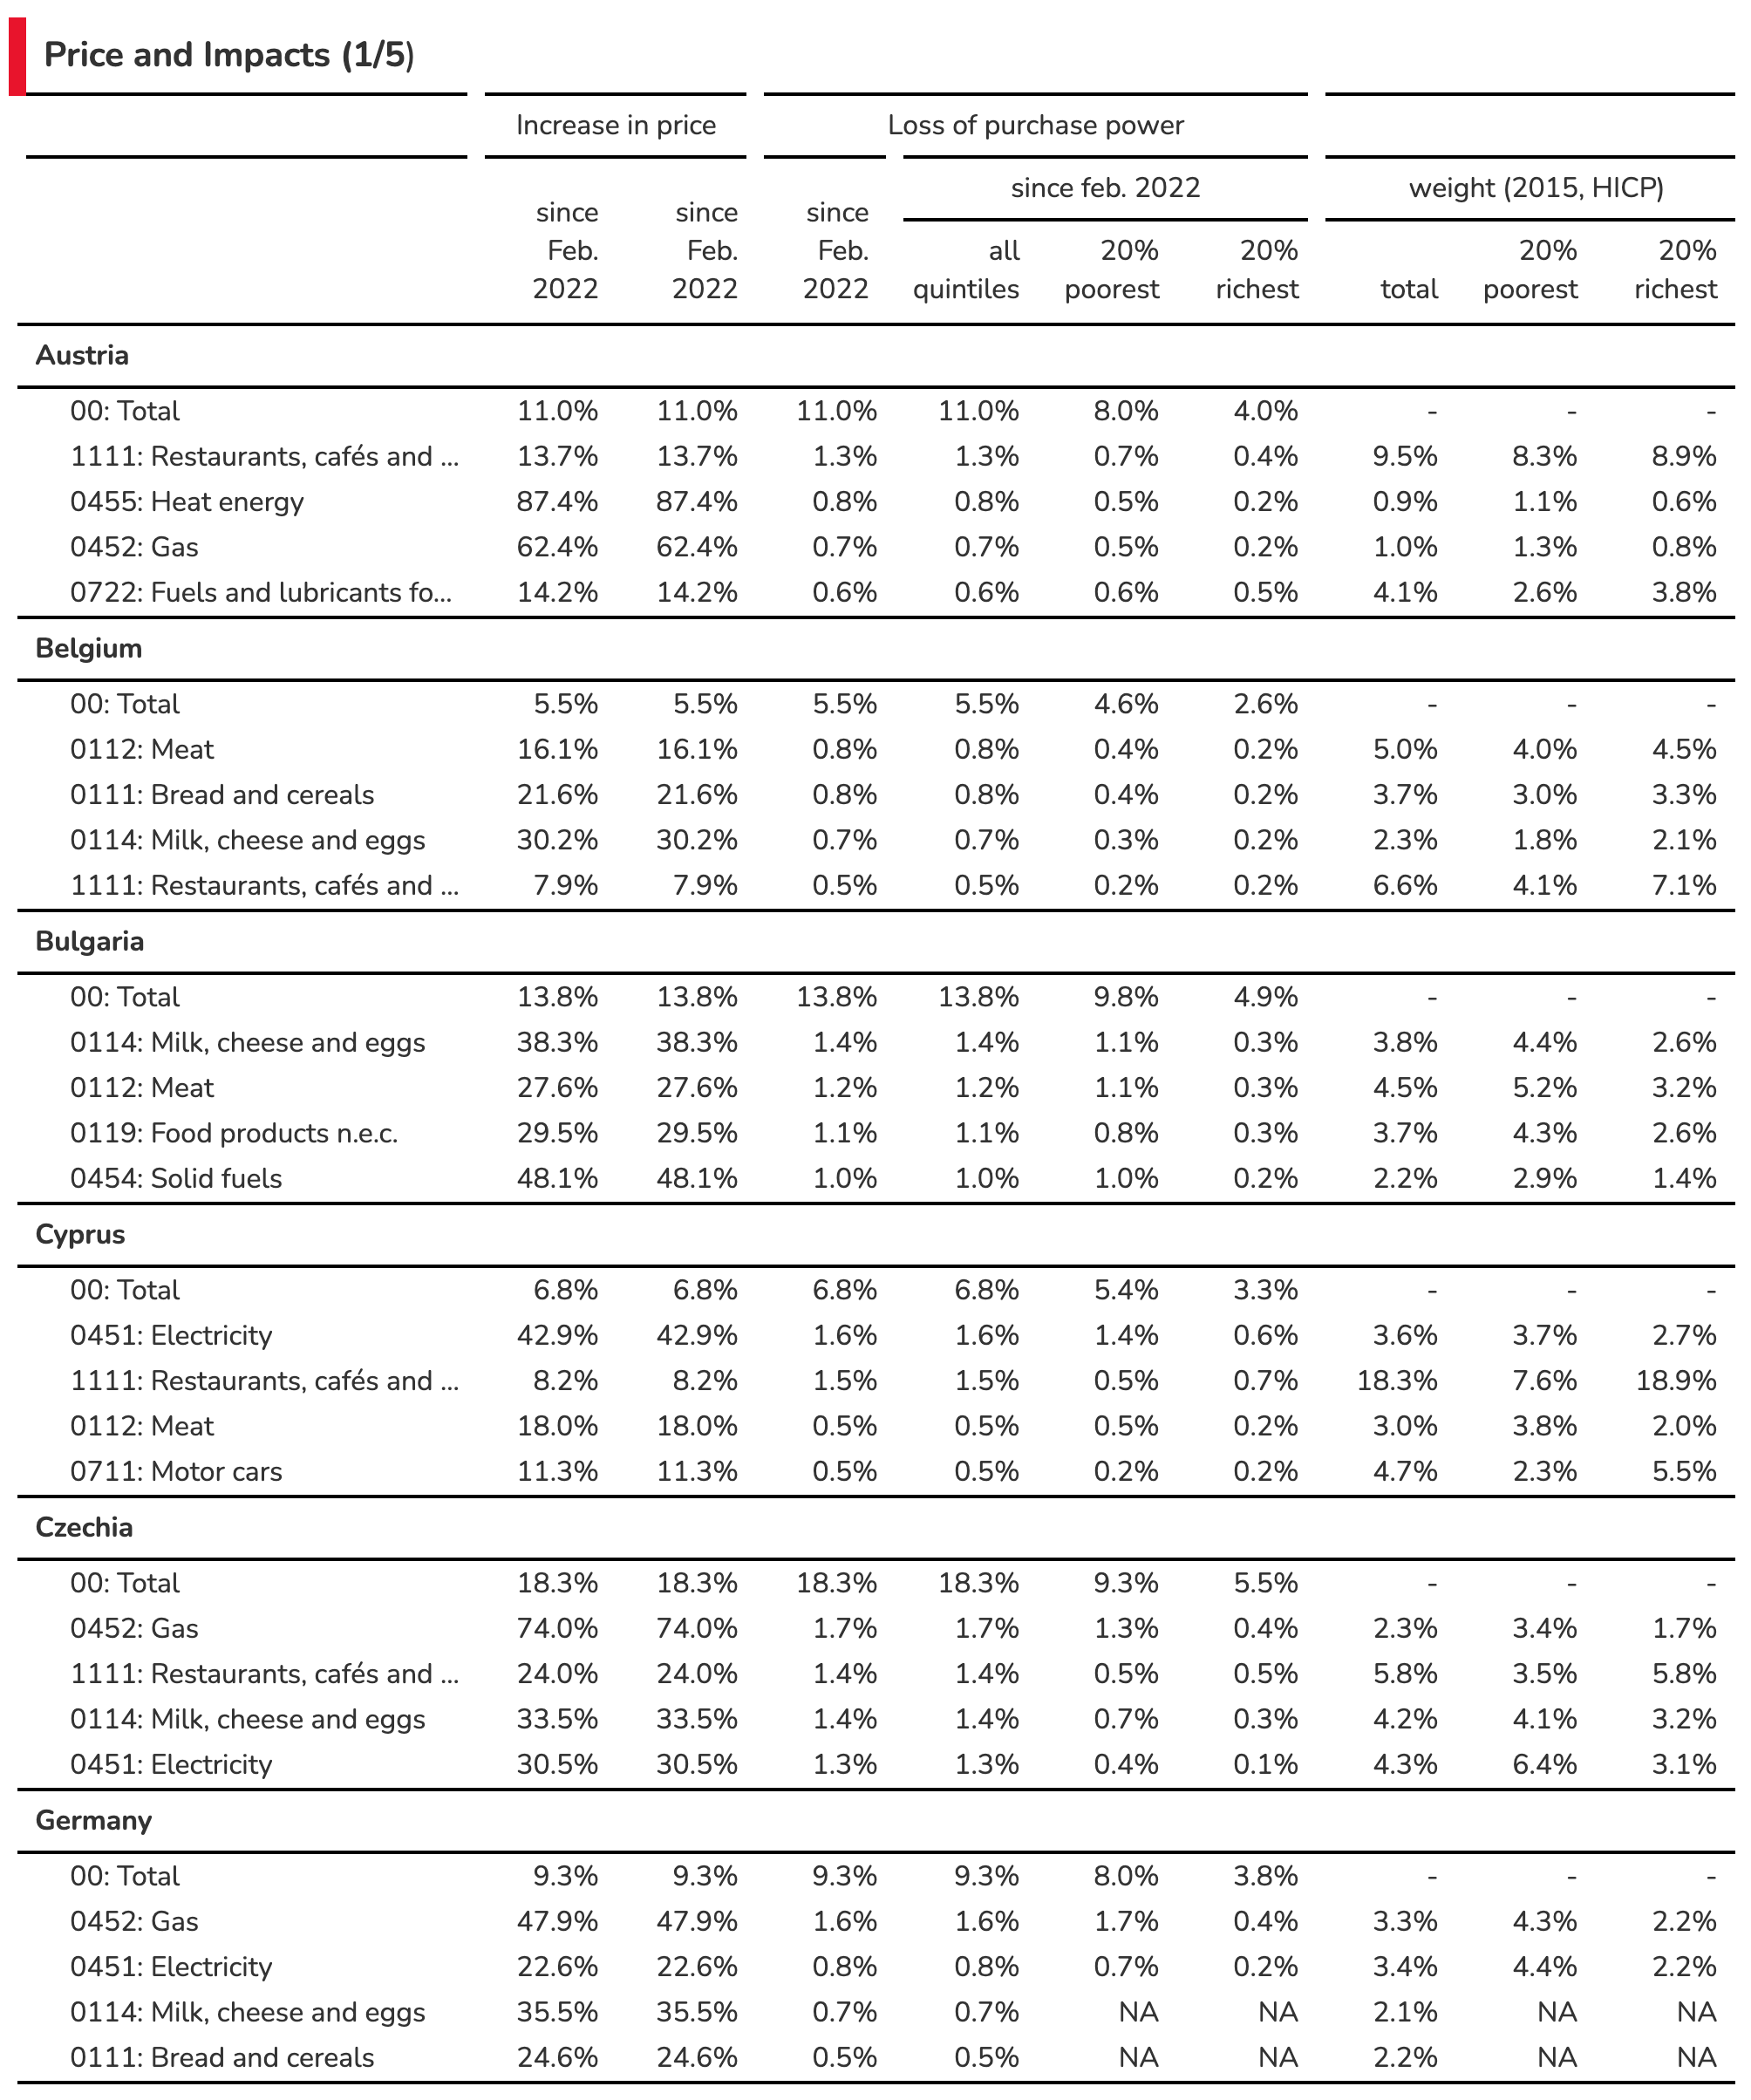
\includegraphics{../svg/annex_1.png}

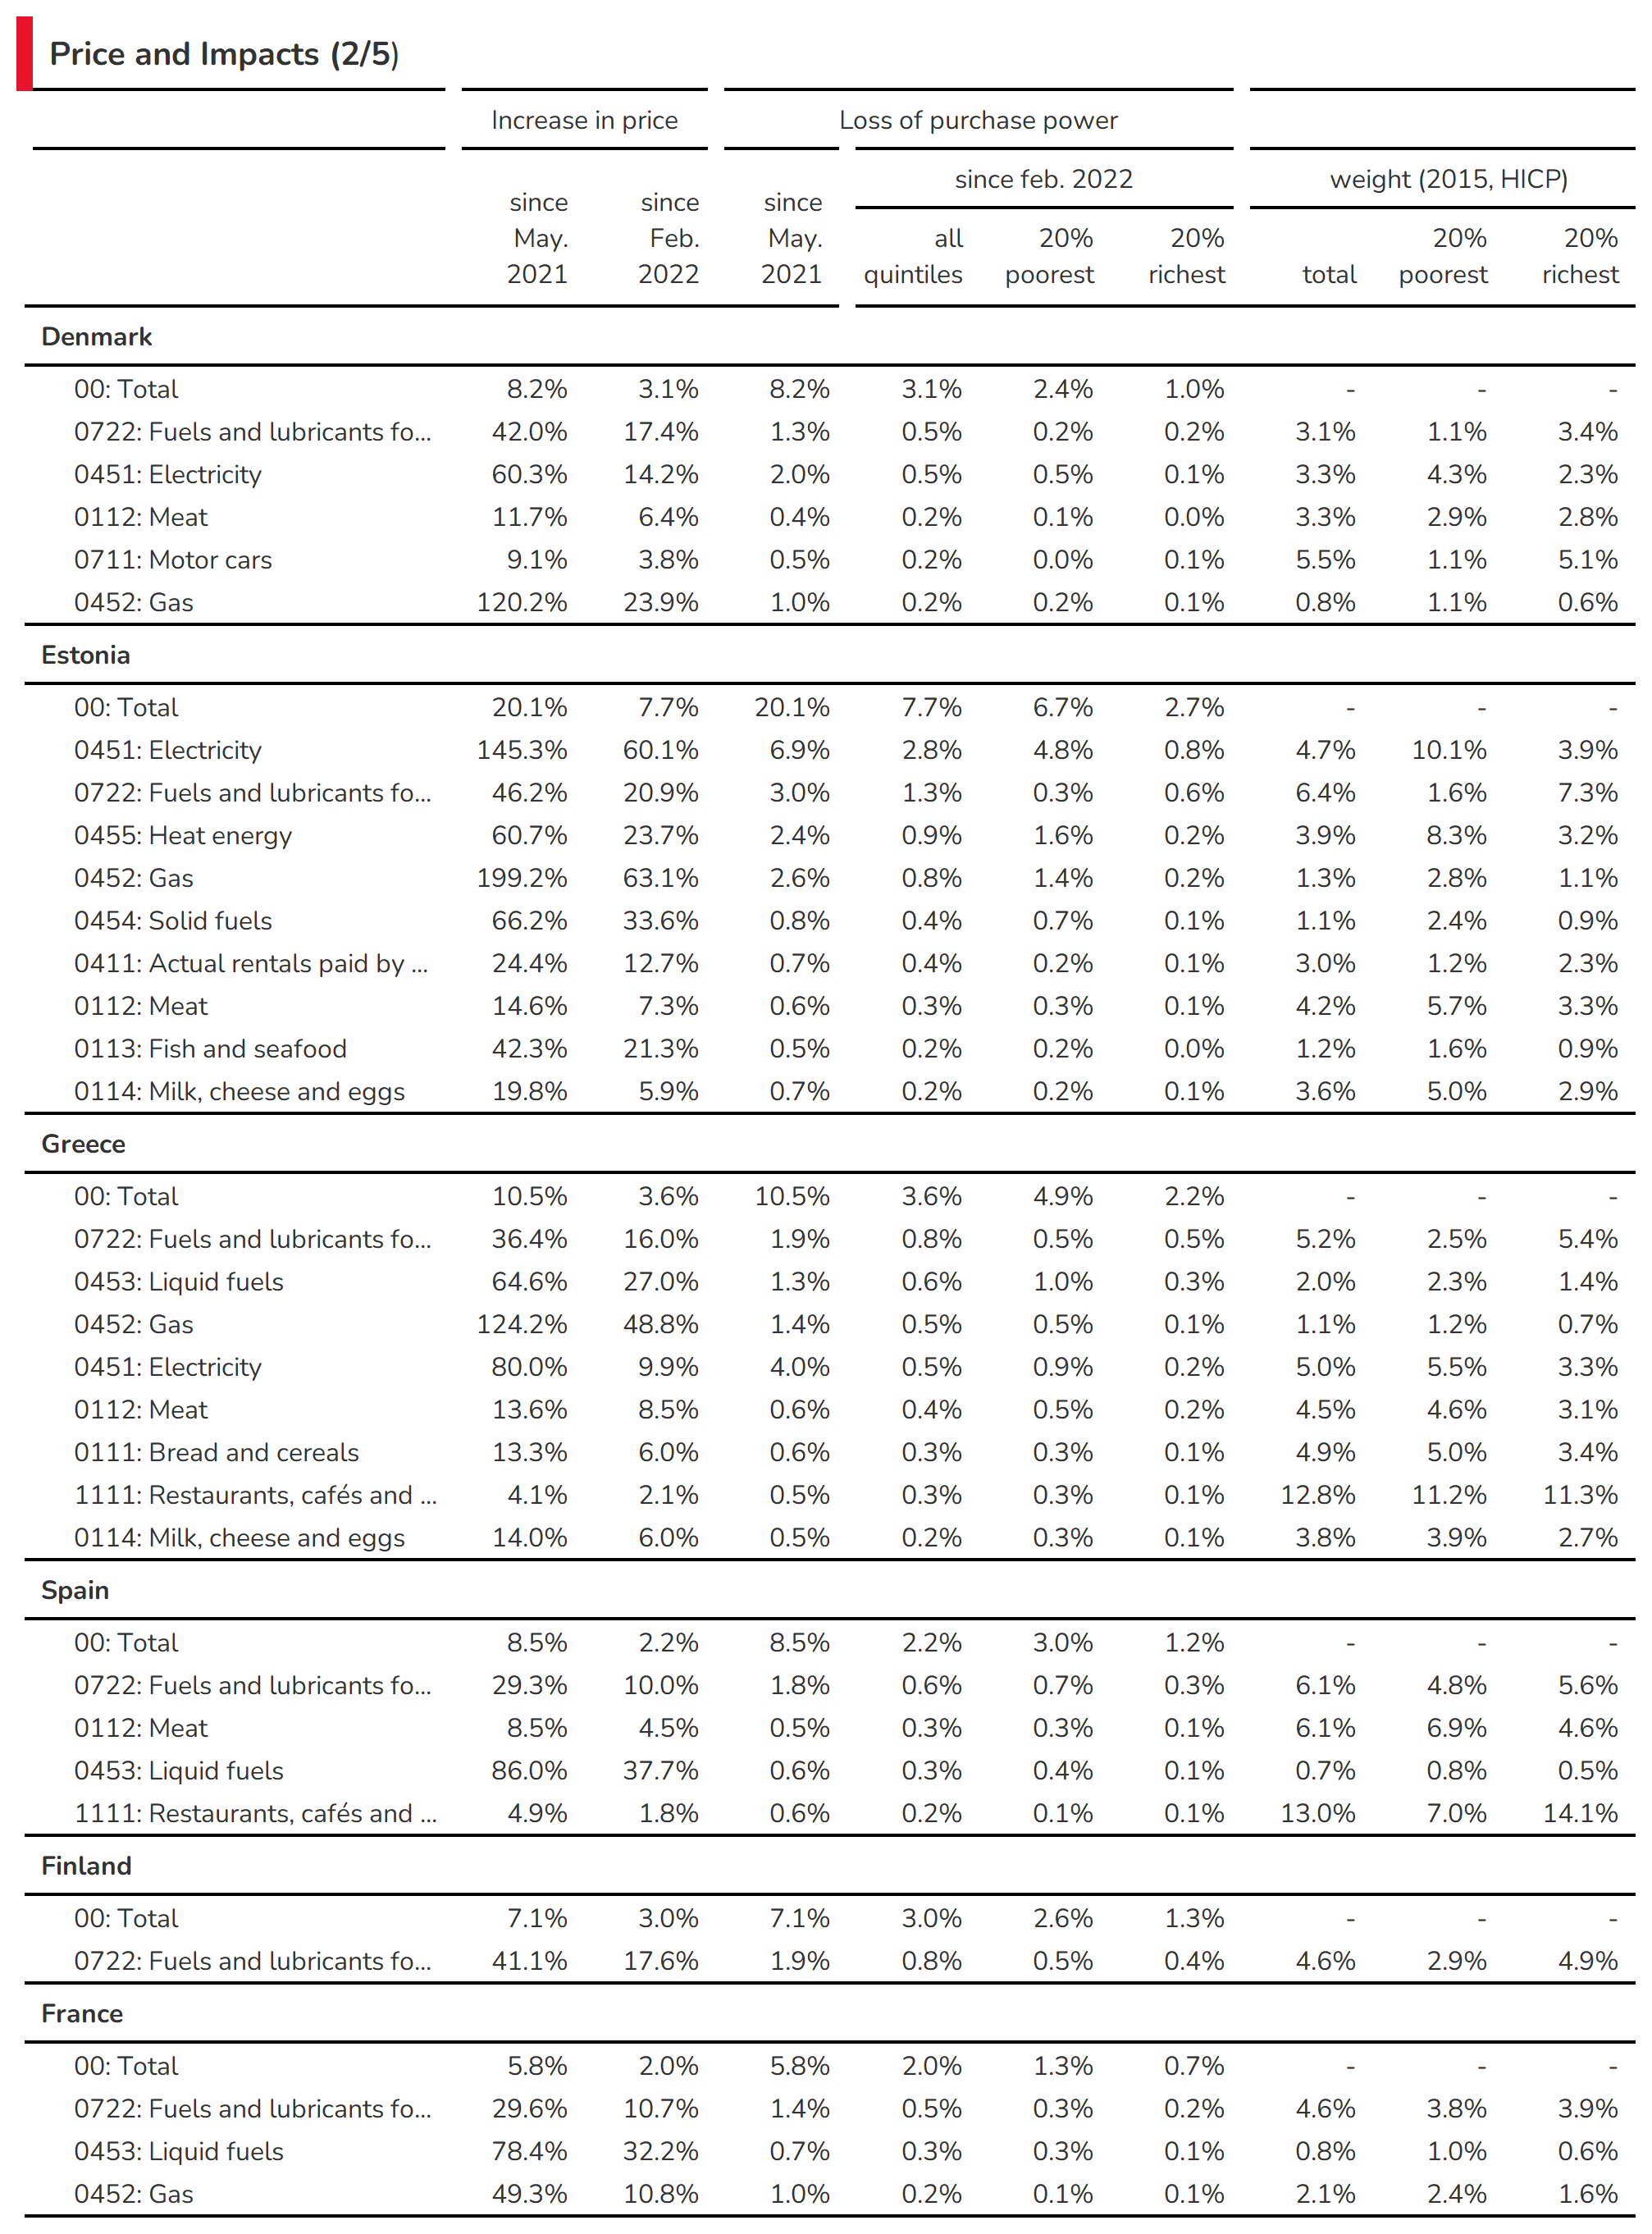
\includegraphics{../svg/annex_2.png}

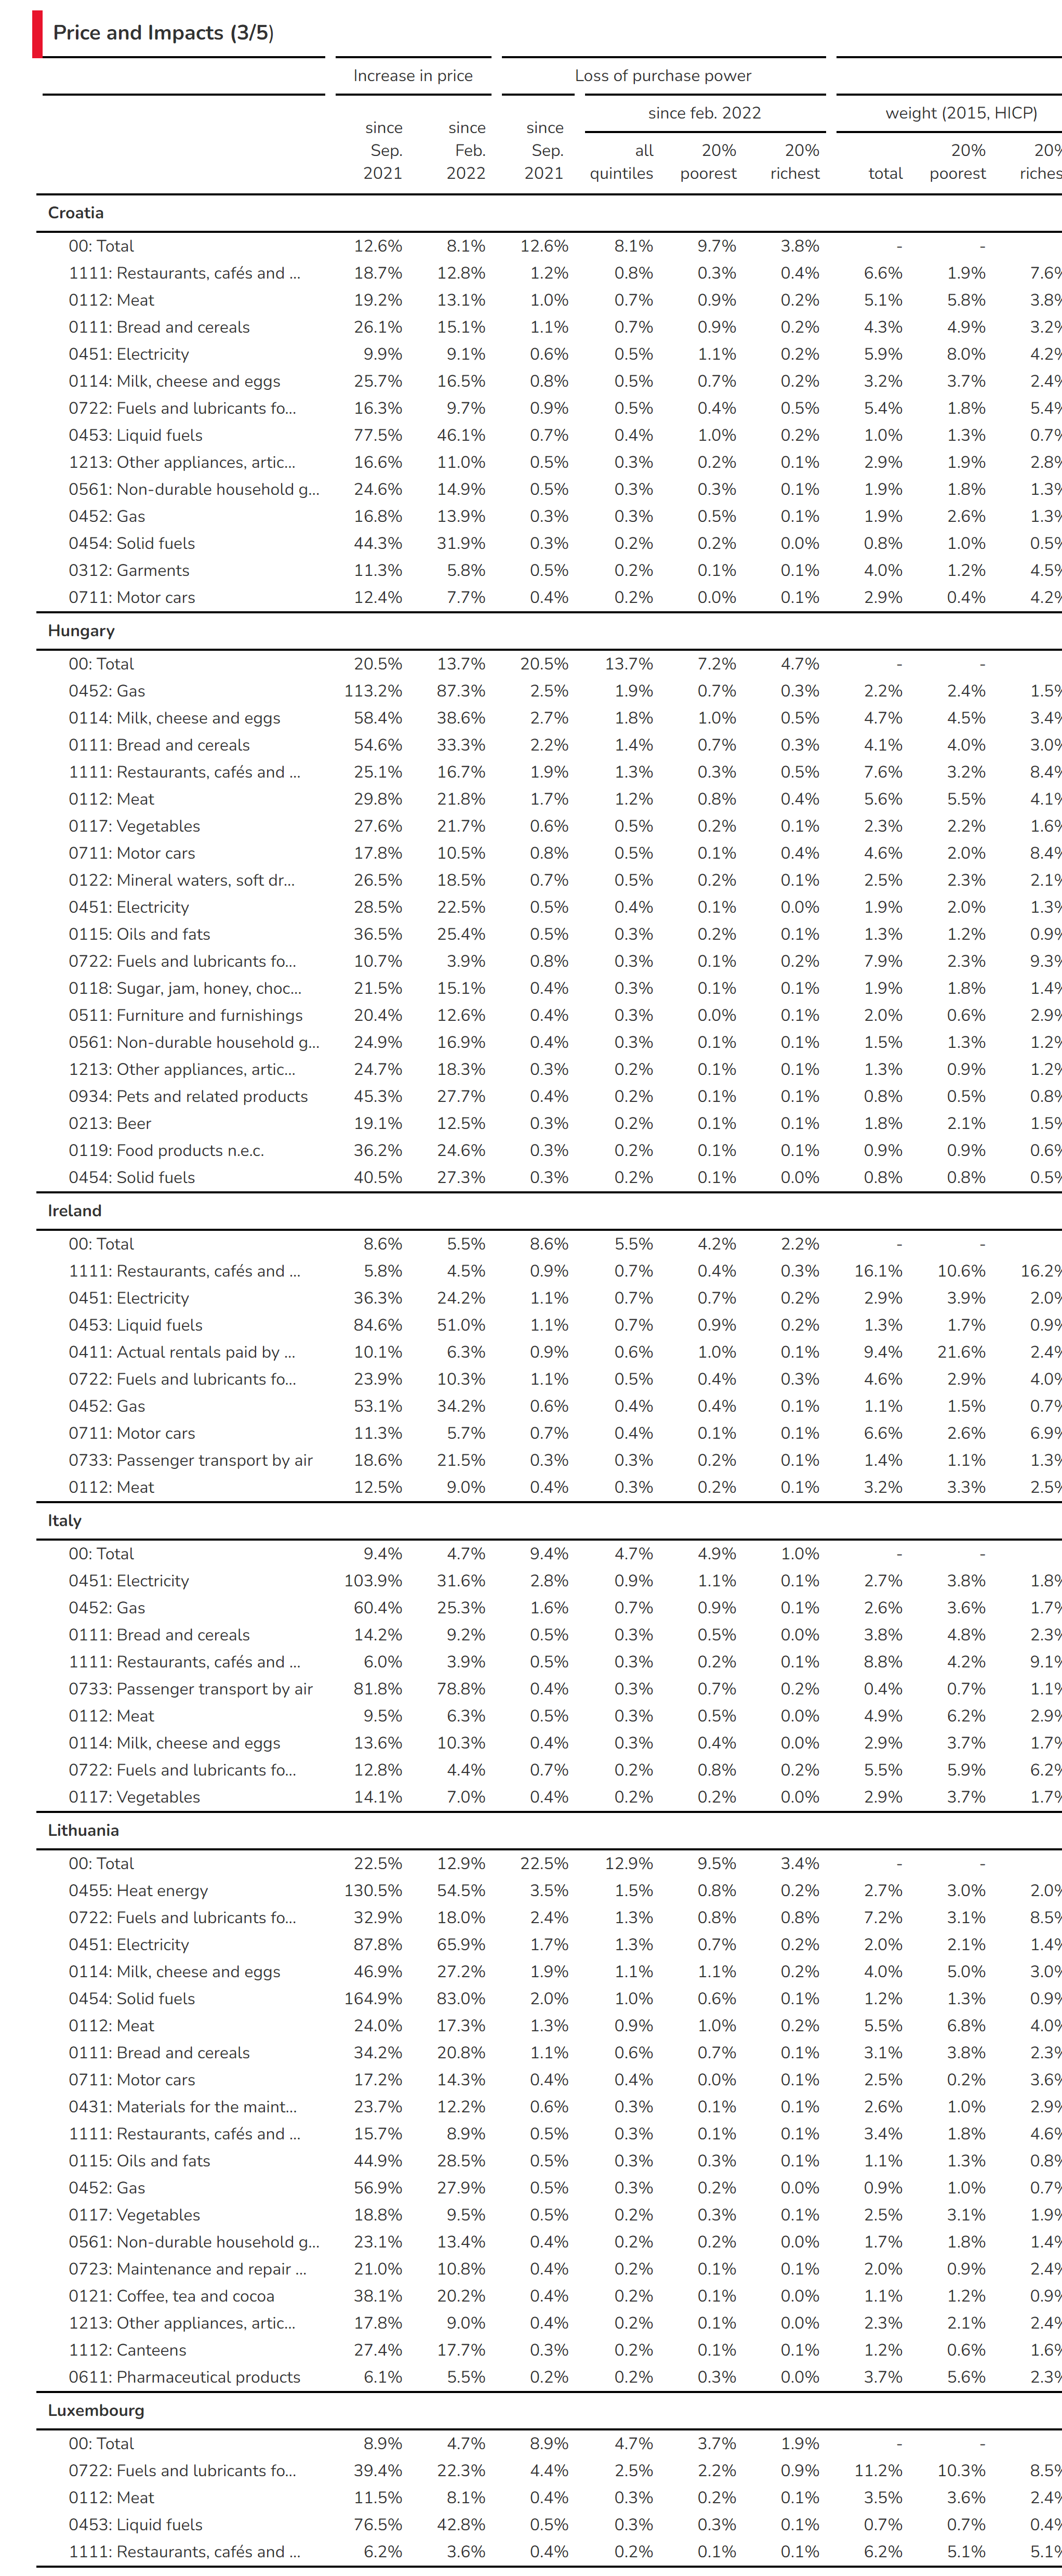
\includegraphics{../svg/annex_3.png}

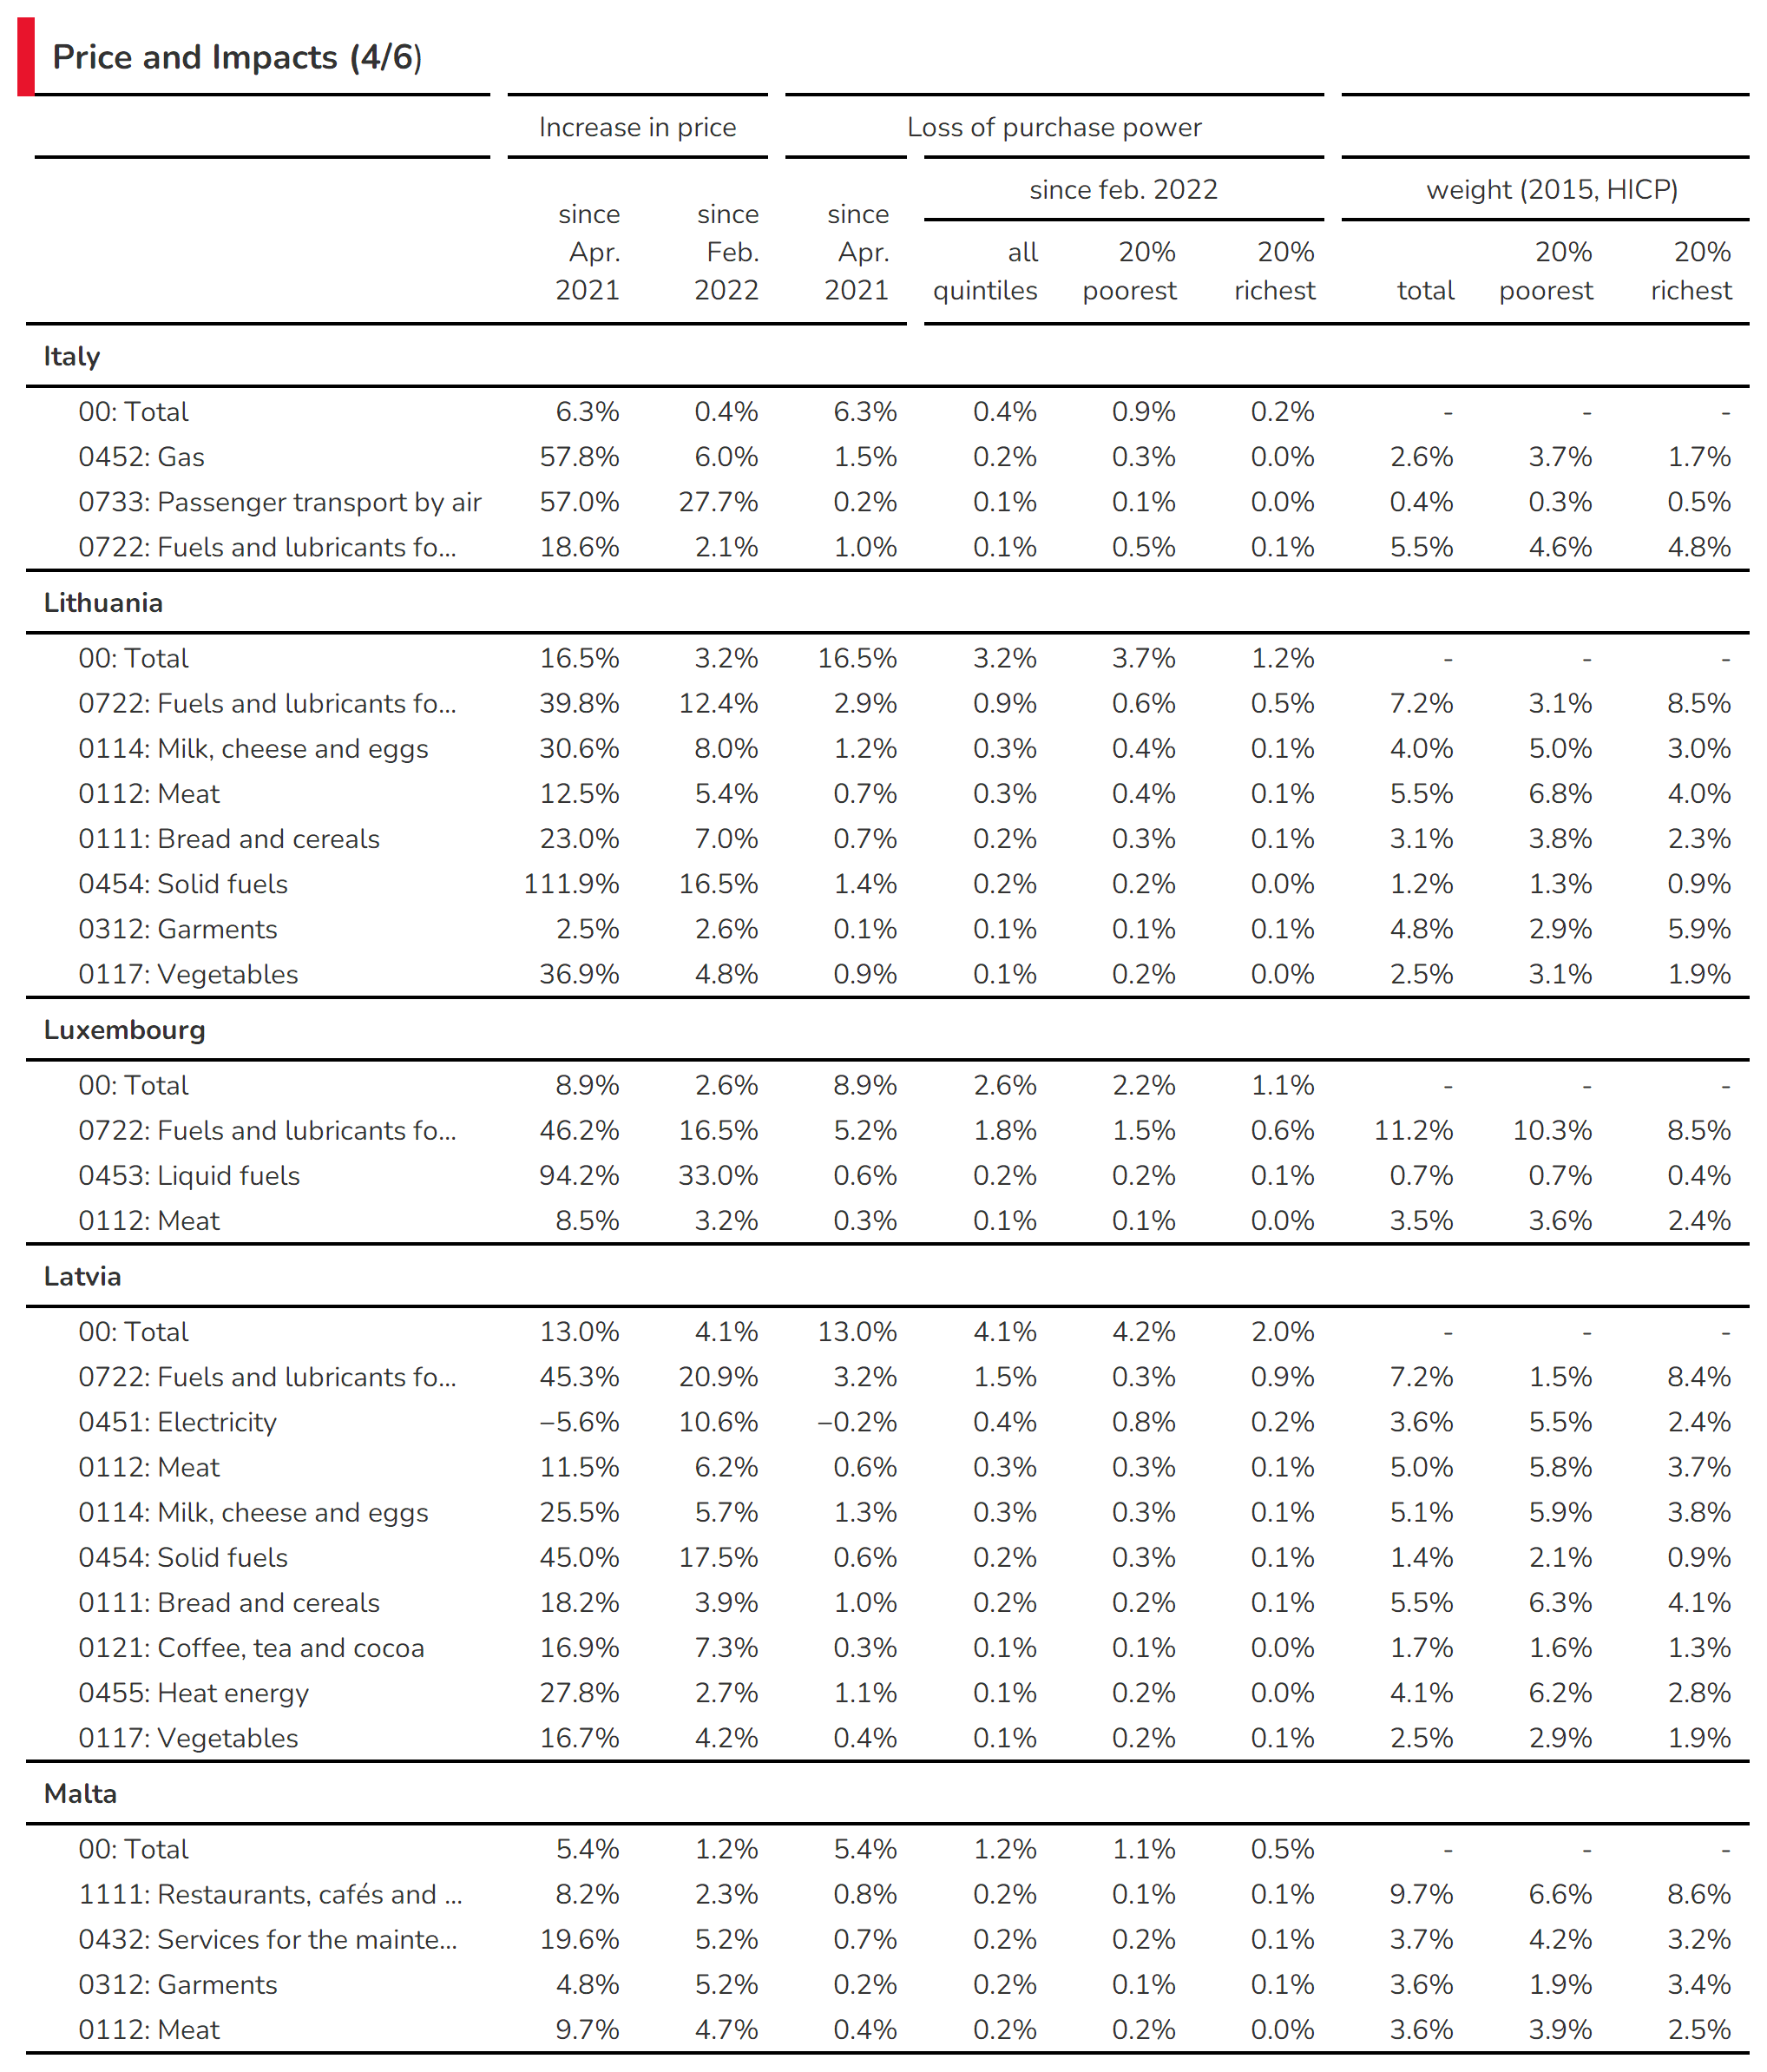
\includegraphics{../svg/annex_4.png}

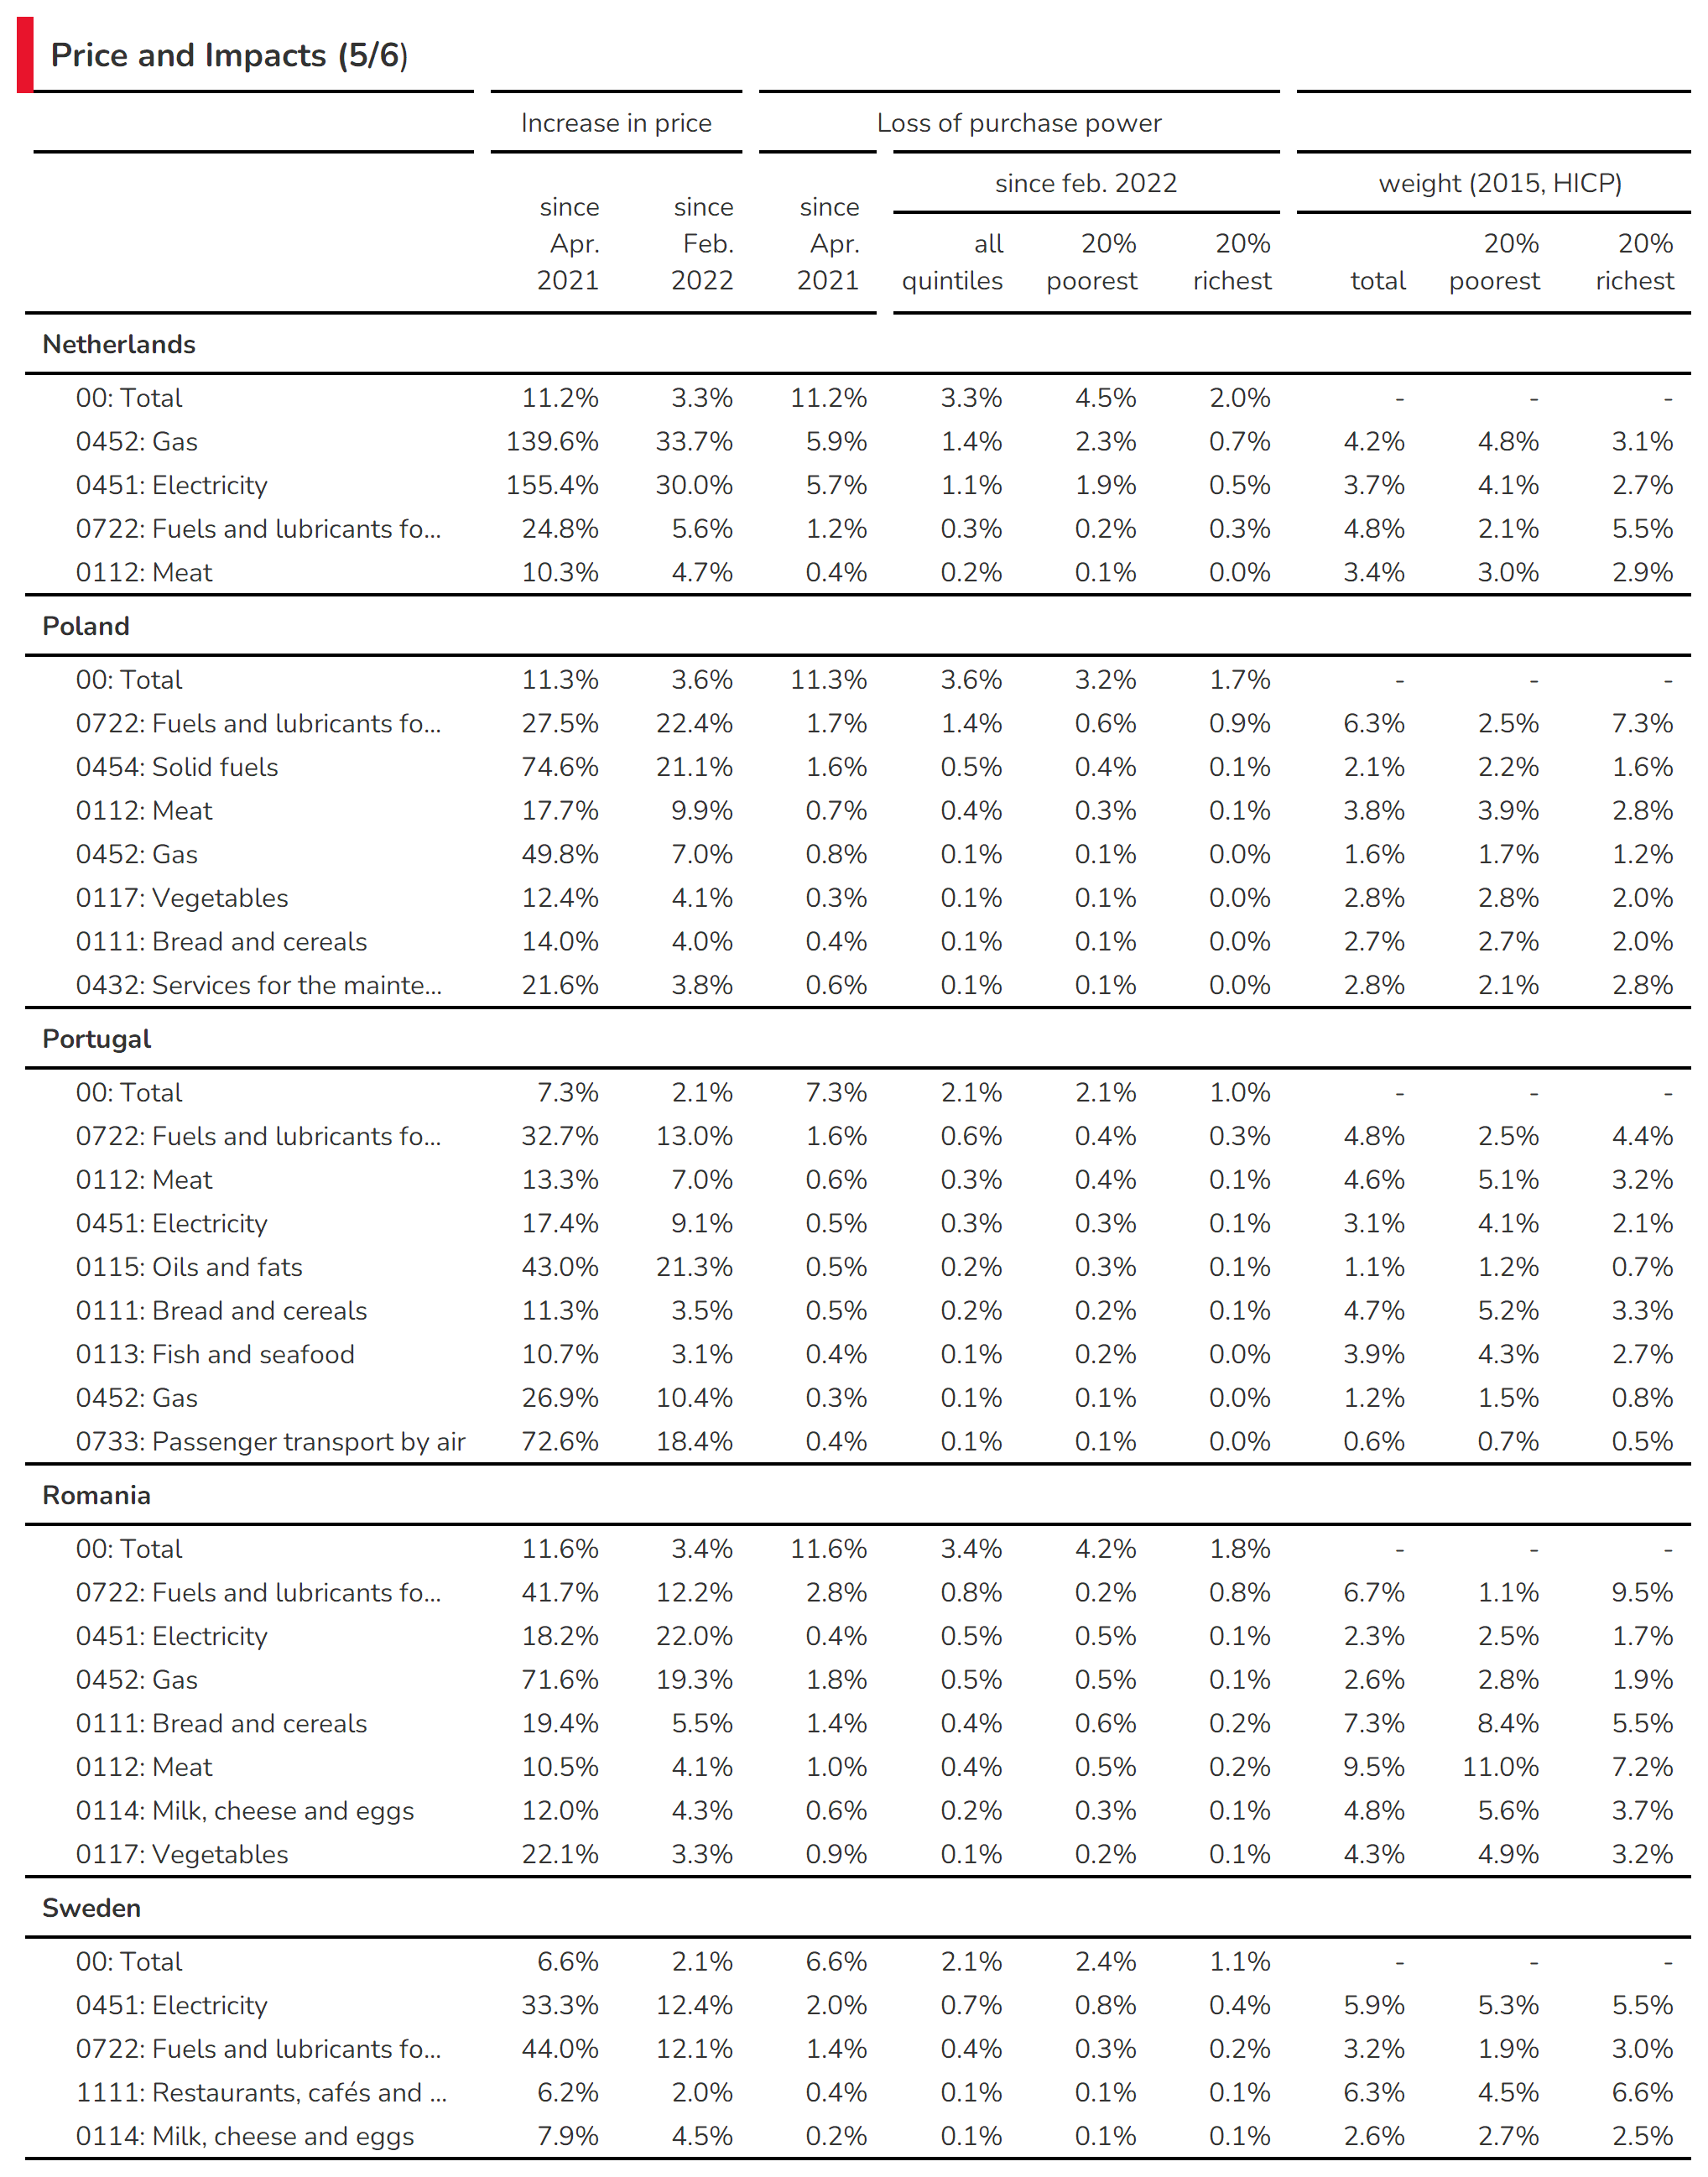
\includegraphics{../svg/annex_5.png}

\newpage

\hypertarget{figures-over-a-one-year-period}{%
\subsection{Figures over a one year
period}\label{figures-over-a-one-year-period}}

\begin{figure}

\caption{Price increase since one year (1/3)}

{\centering 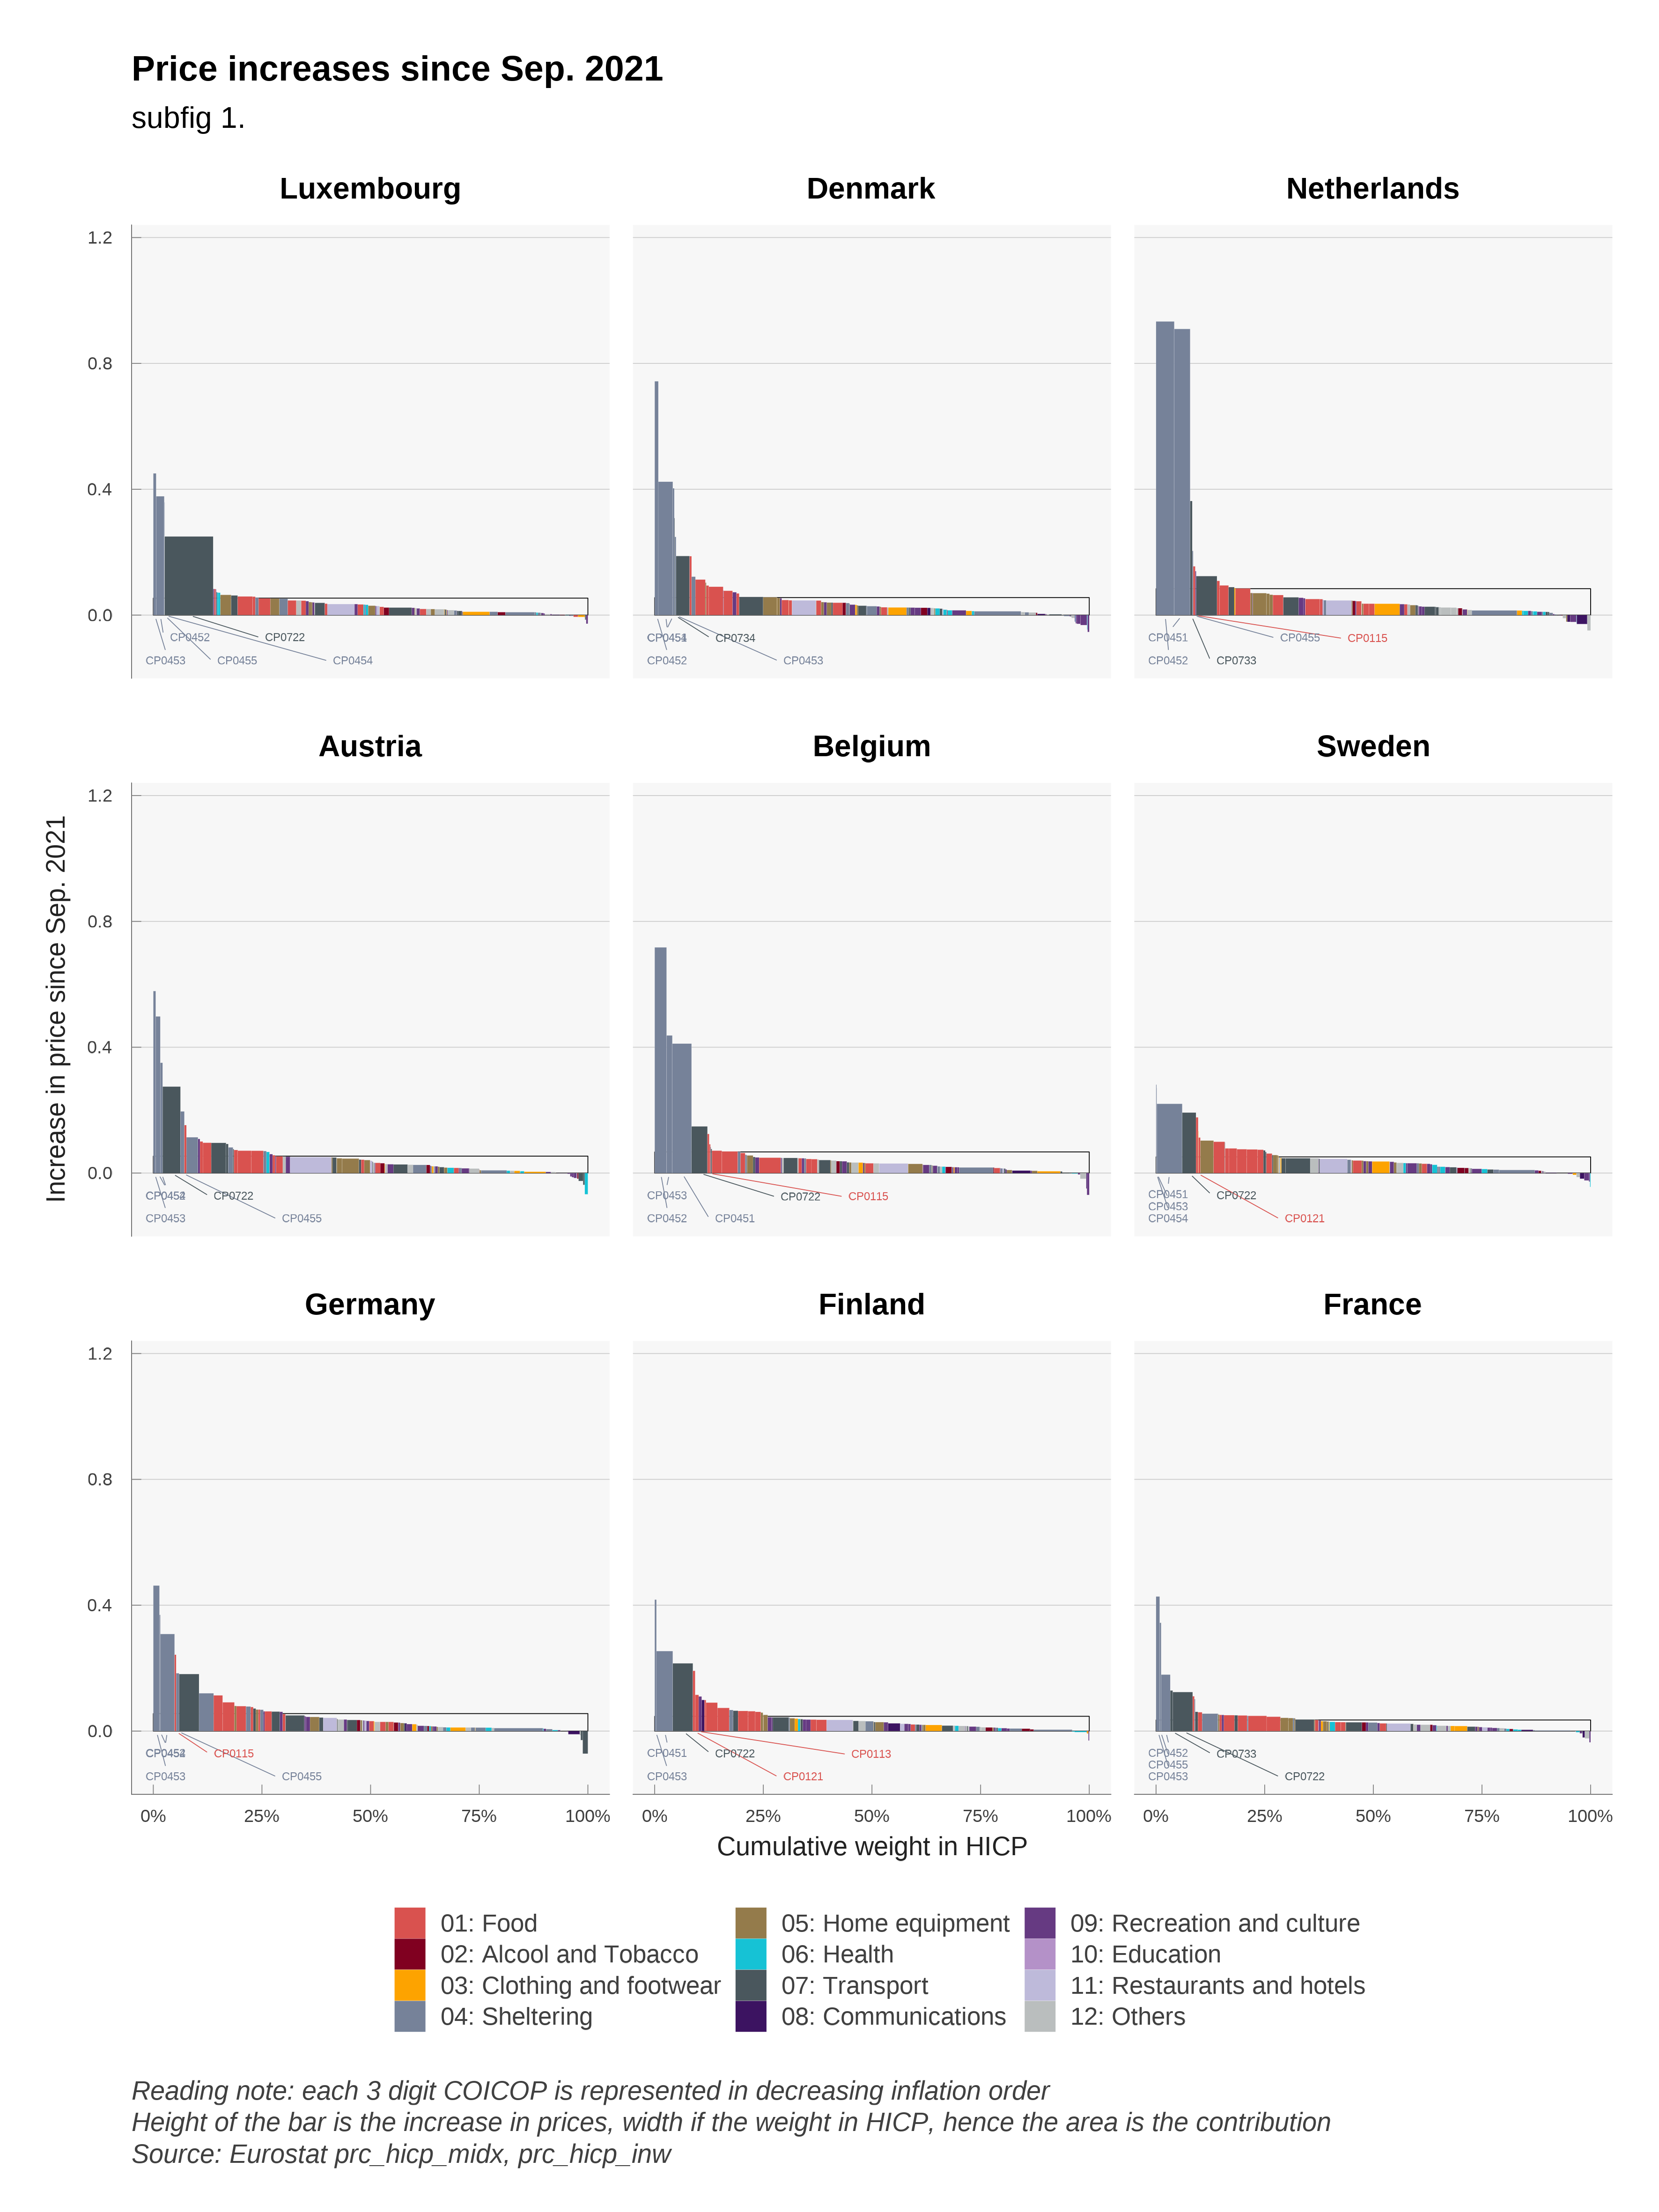
\includegraphics{../svg/depuis_1y_1.png}

}

\end{figure}

\begin{figure}

\caption{Price increase since one year (2/3)}

{\centering 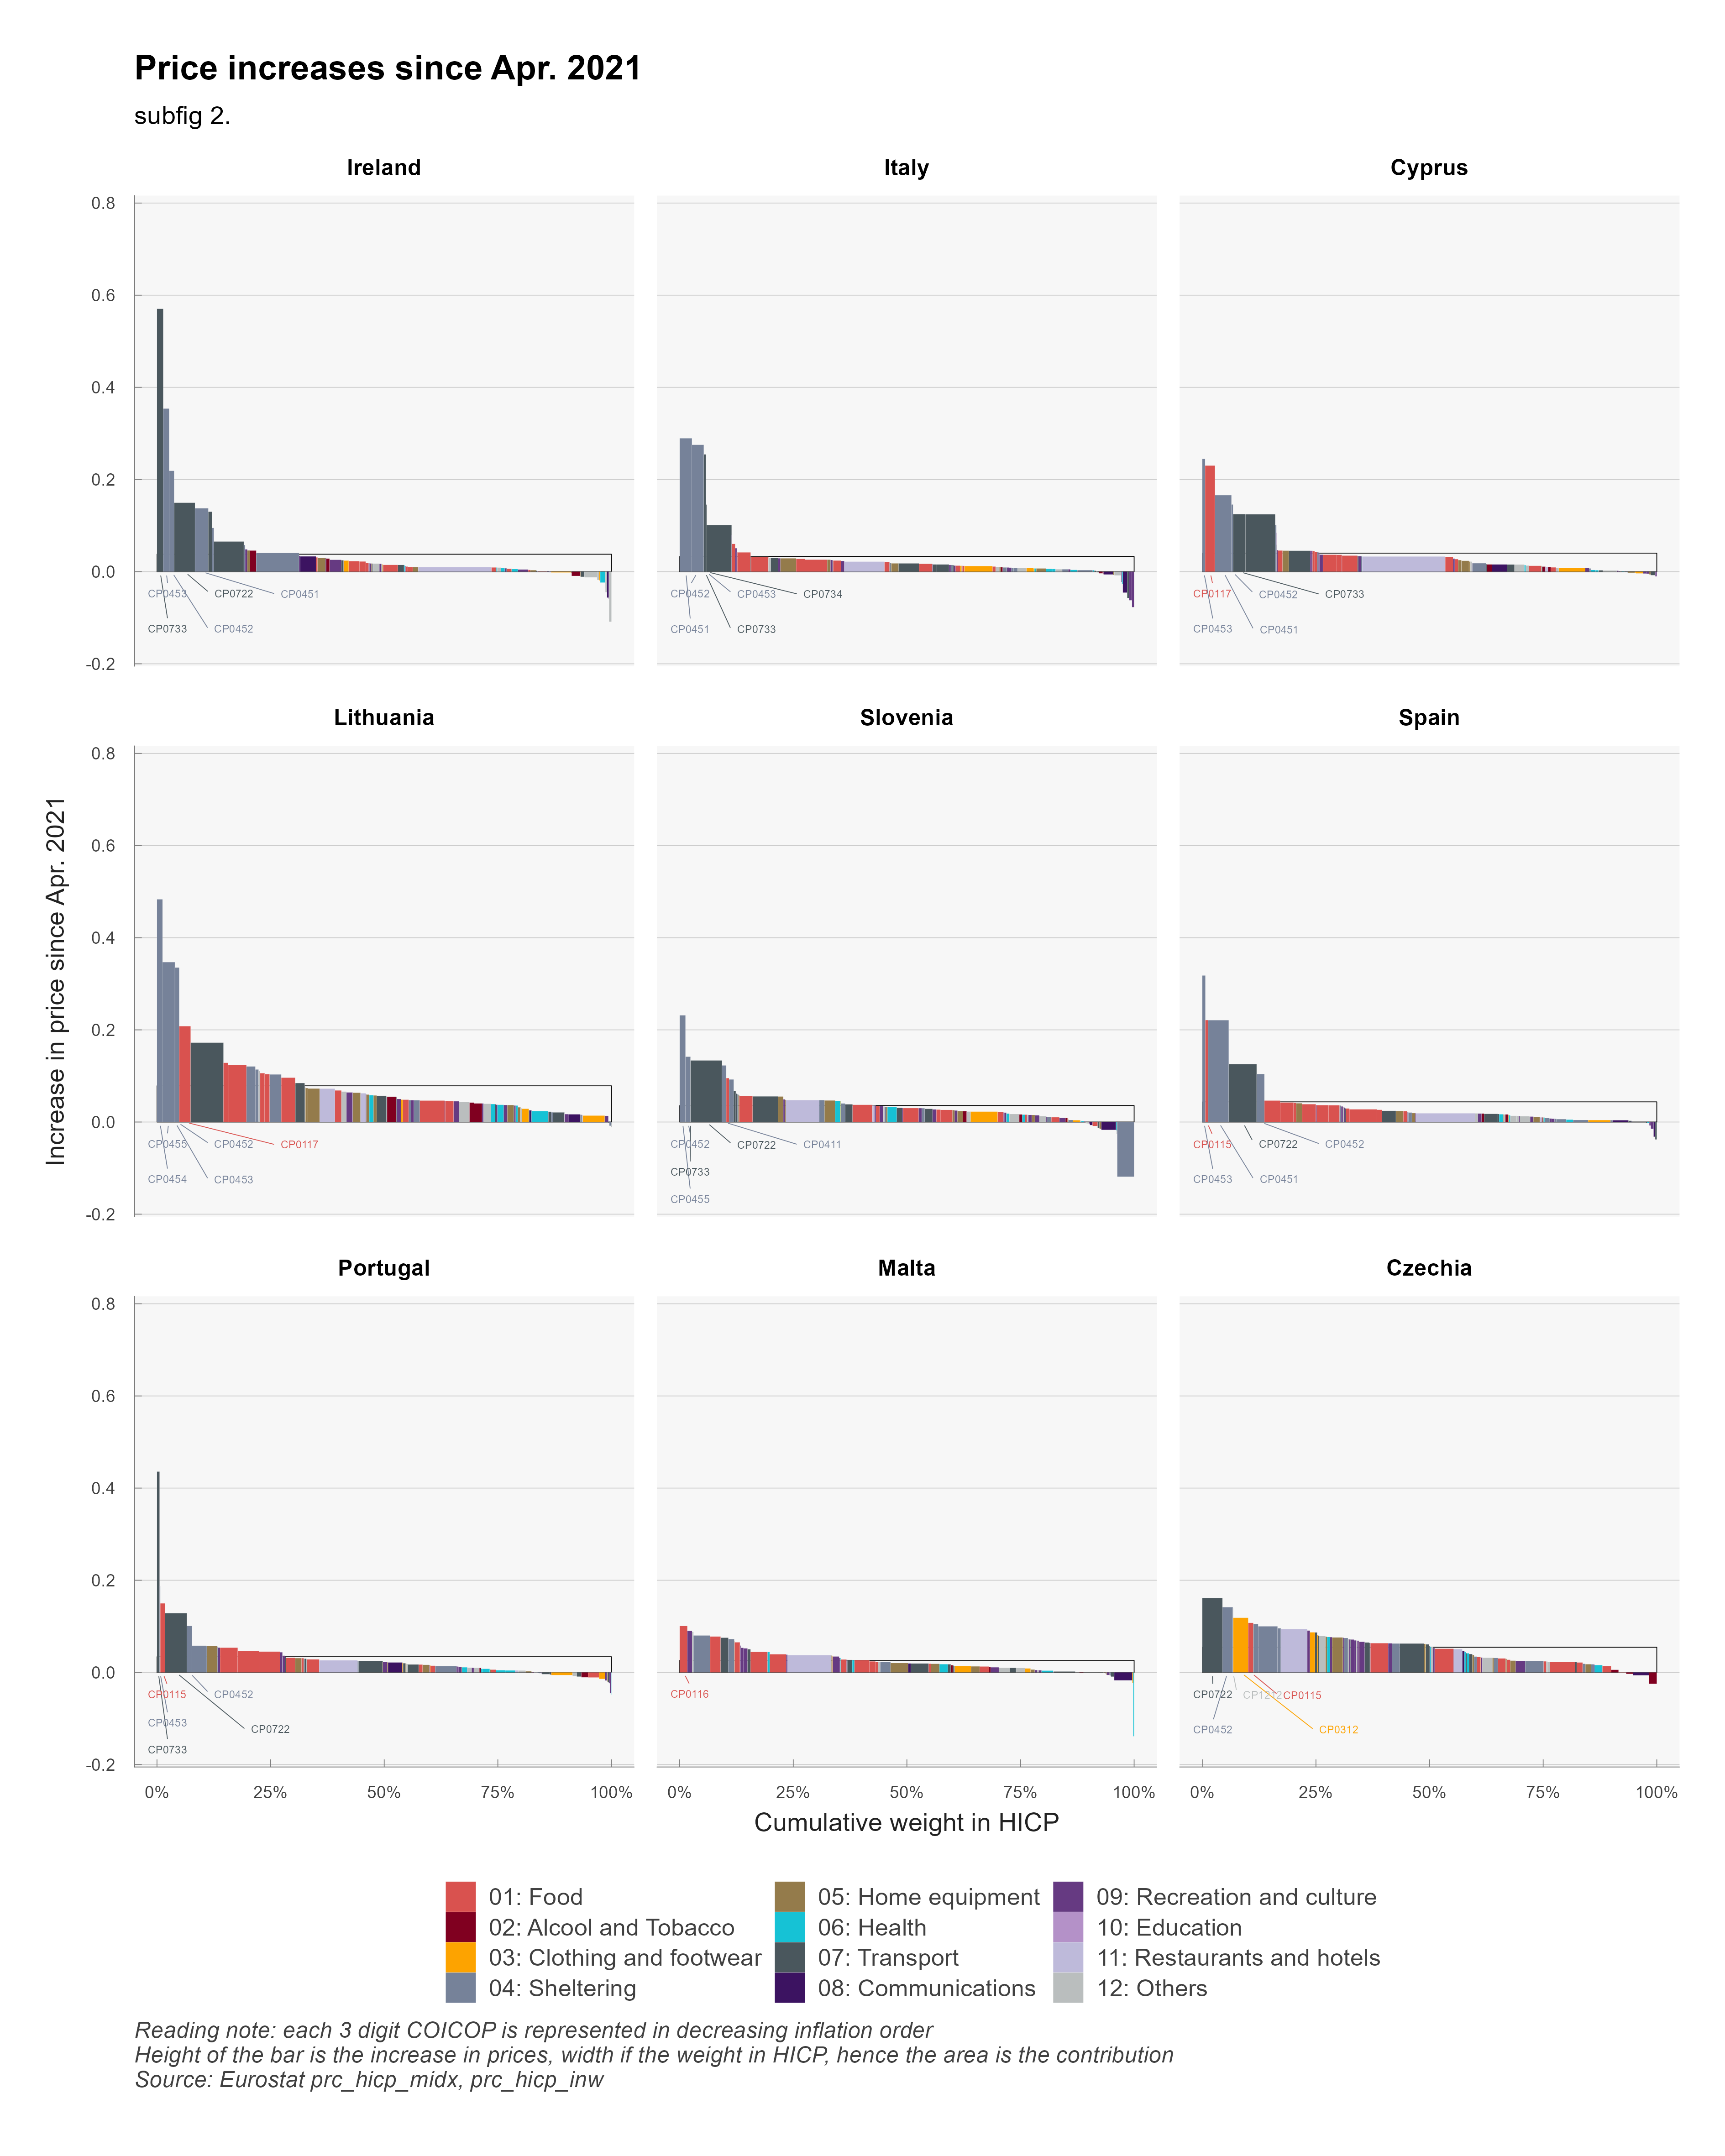
\includegraphics{../svg/depuis_1y_2.png}

}

\end{figure}

\begin{figure}

\caption{Price increase since War one year (3/3)}

{\centering 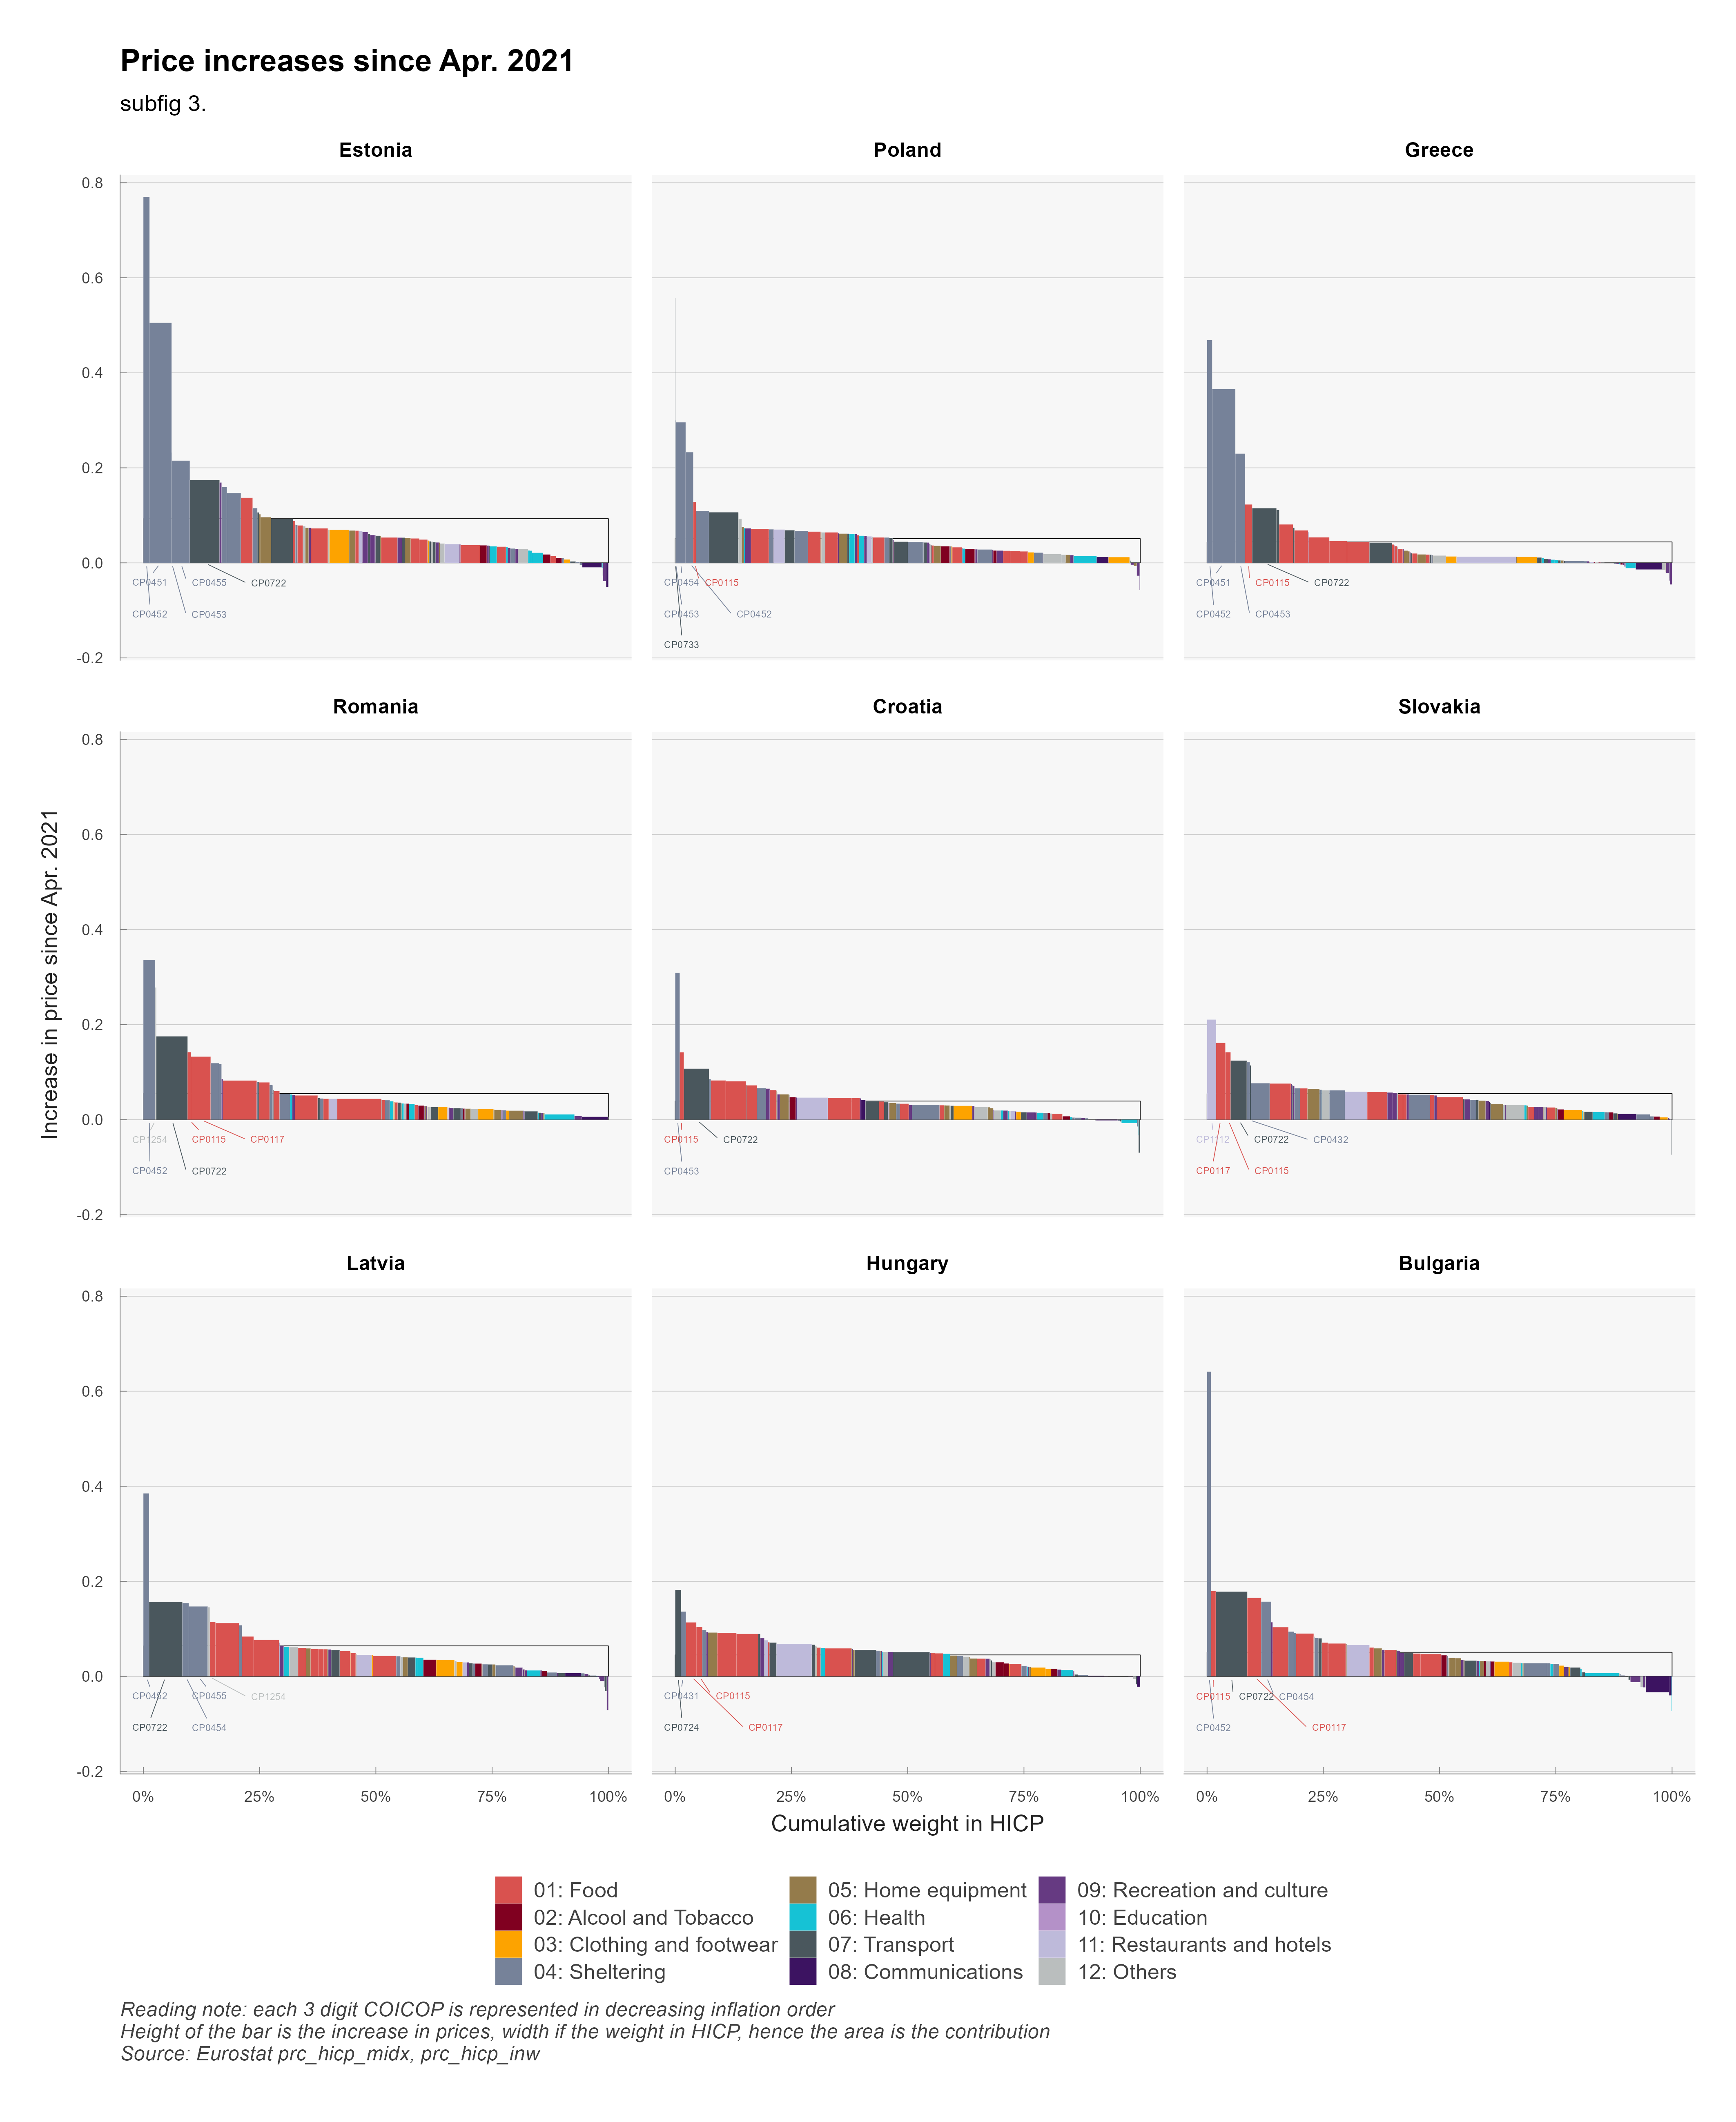
\includegraphics{../svg/depuis_1y_3.png}

}

\end{figure}

\begin{figure}

\caption{Impact on income per quintile (1/3)}

{\centering 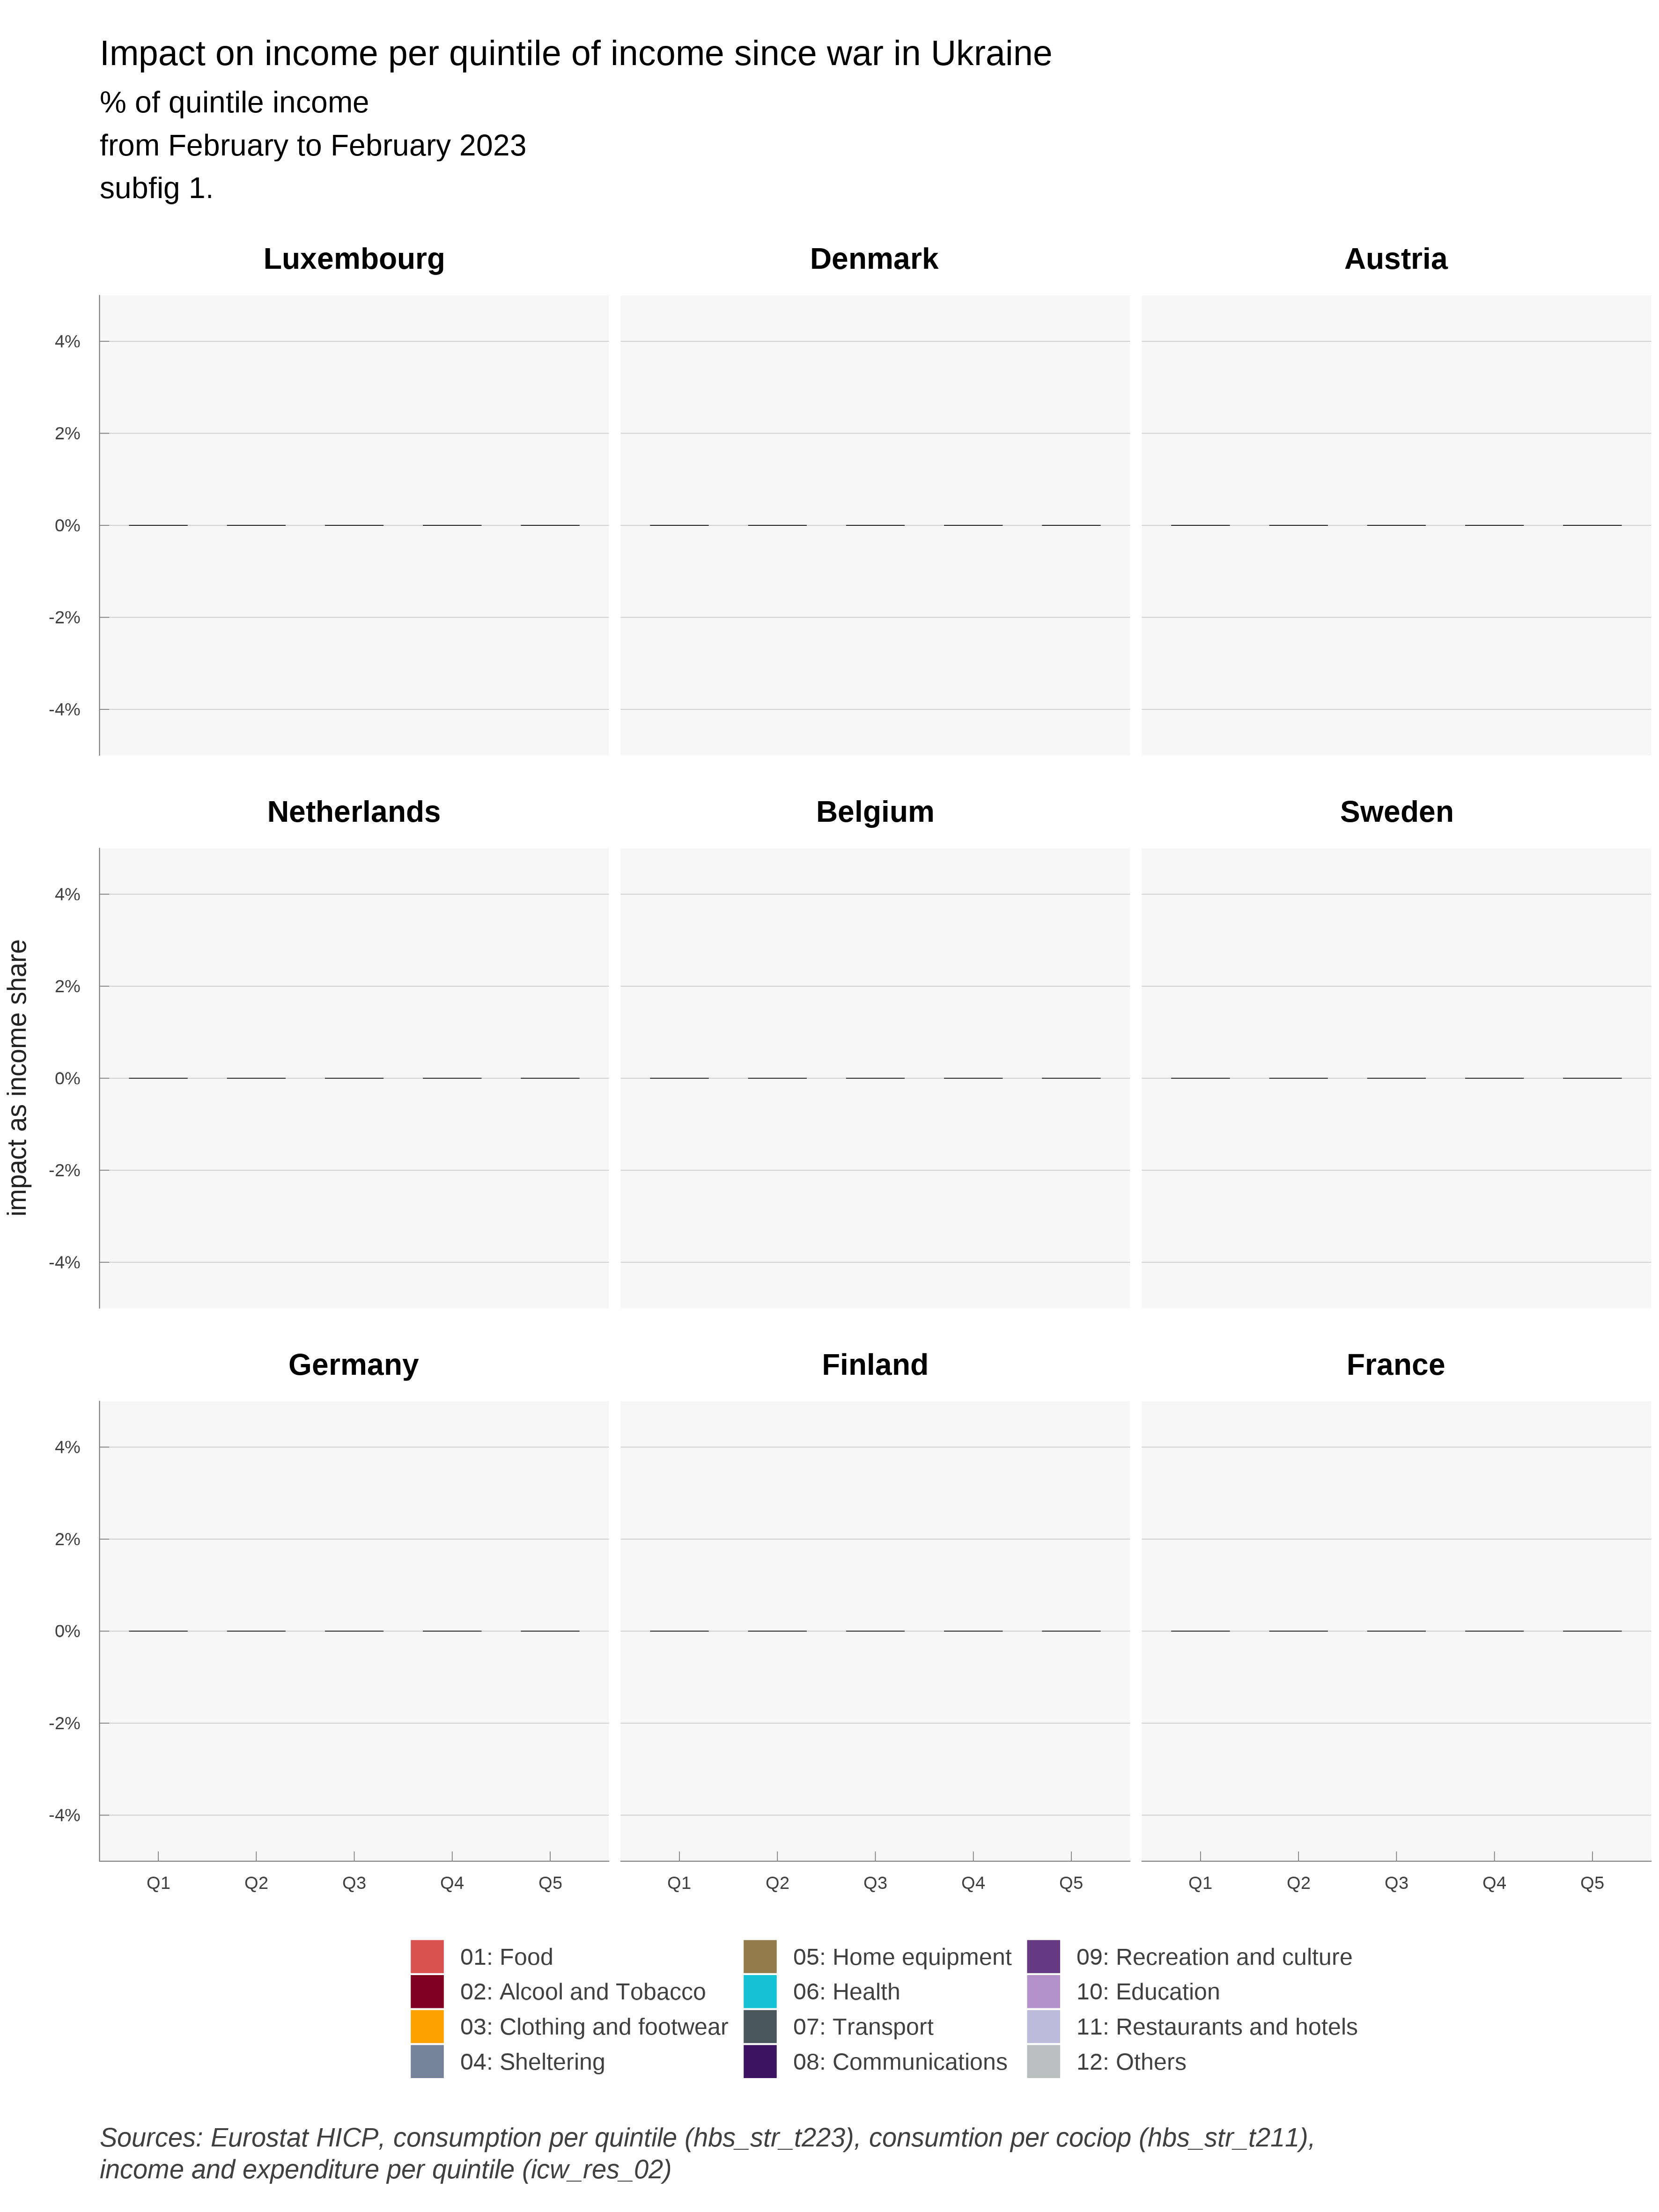
\includegraphics{../svg/coicop_l1_1y_1.png}

}

\end{figure}

\begin{figure}

\caption{Impact on income per quintile (2/3)}

{\centering 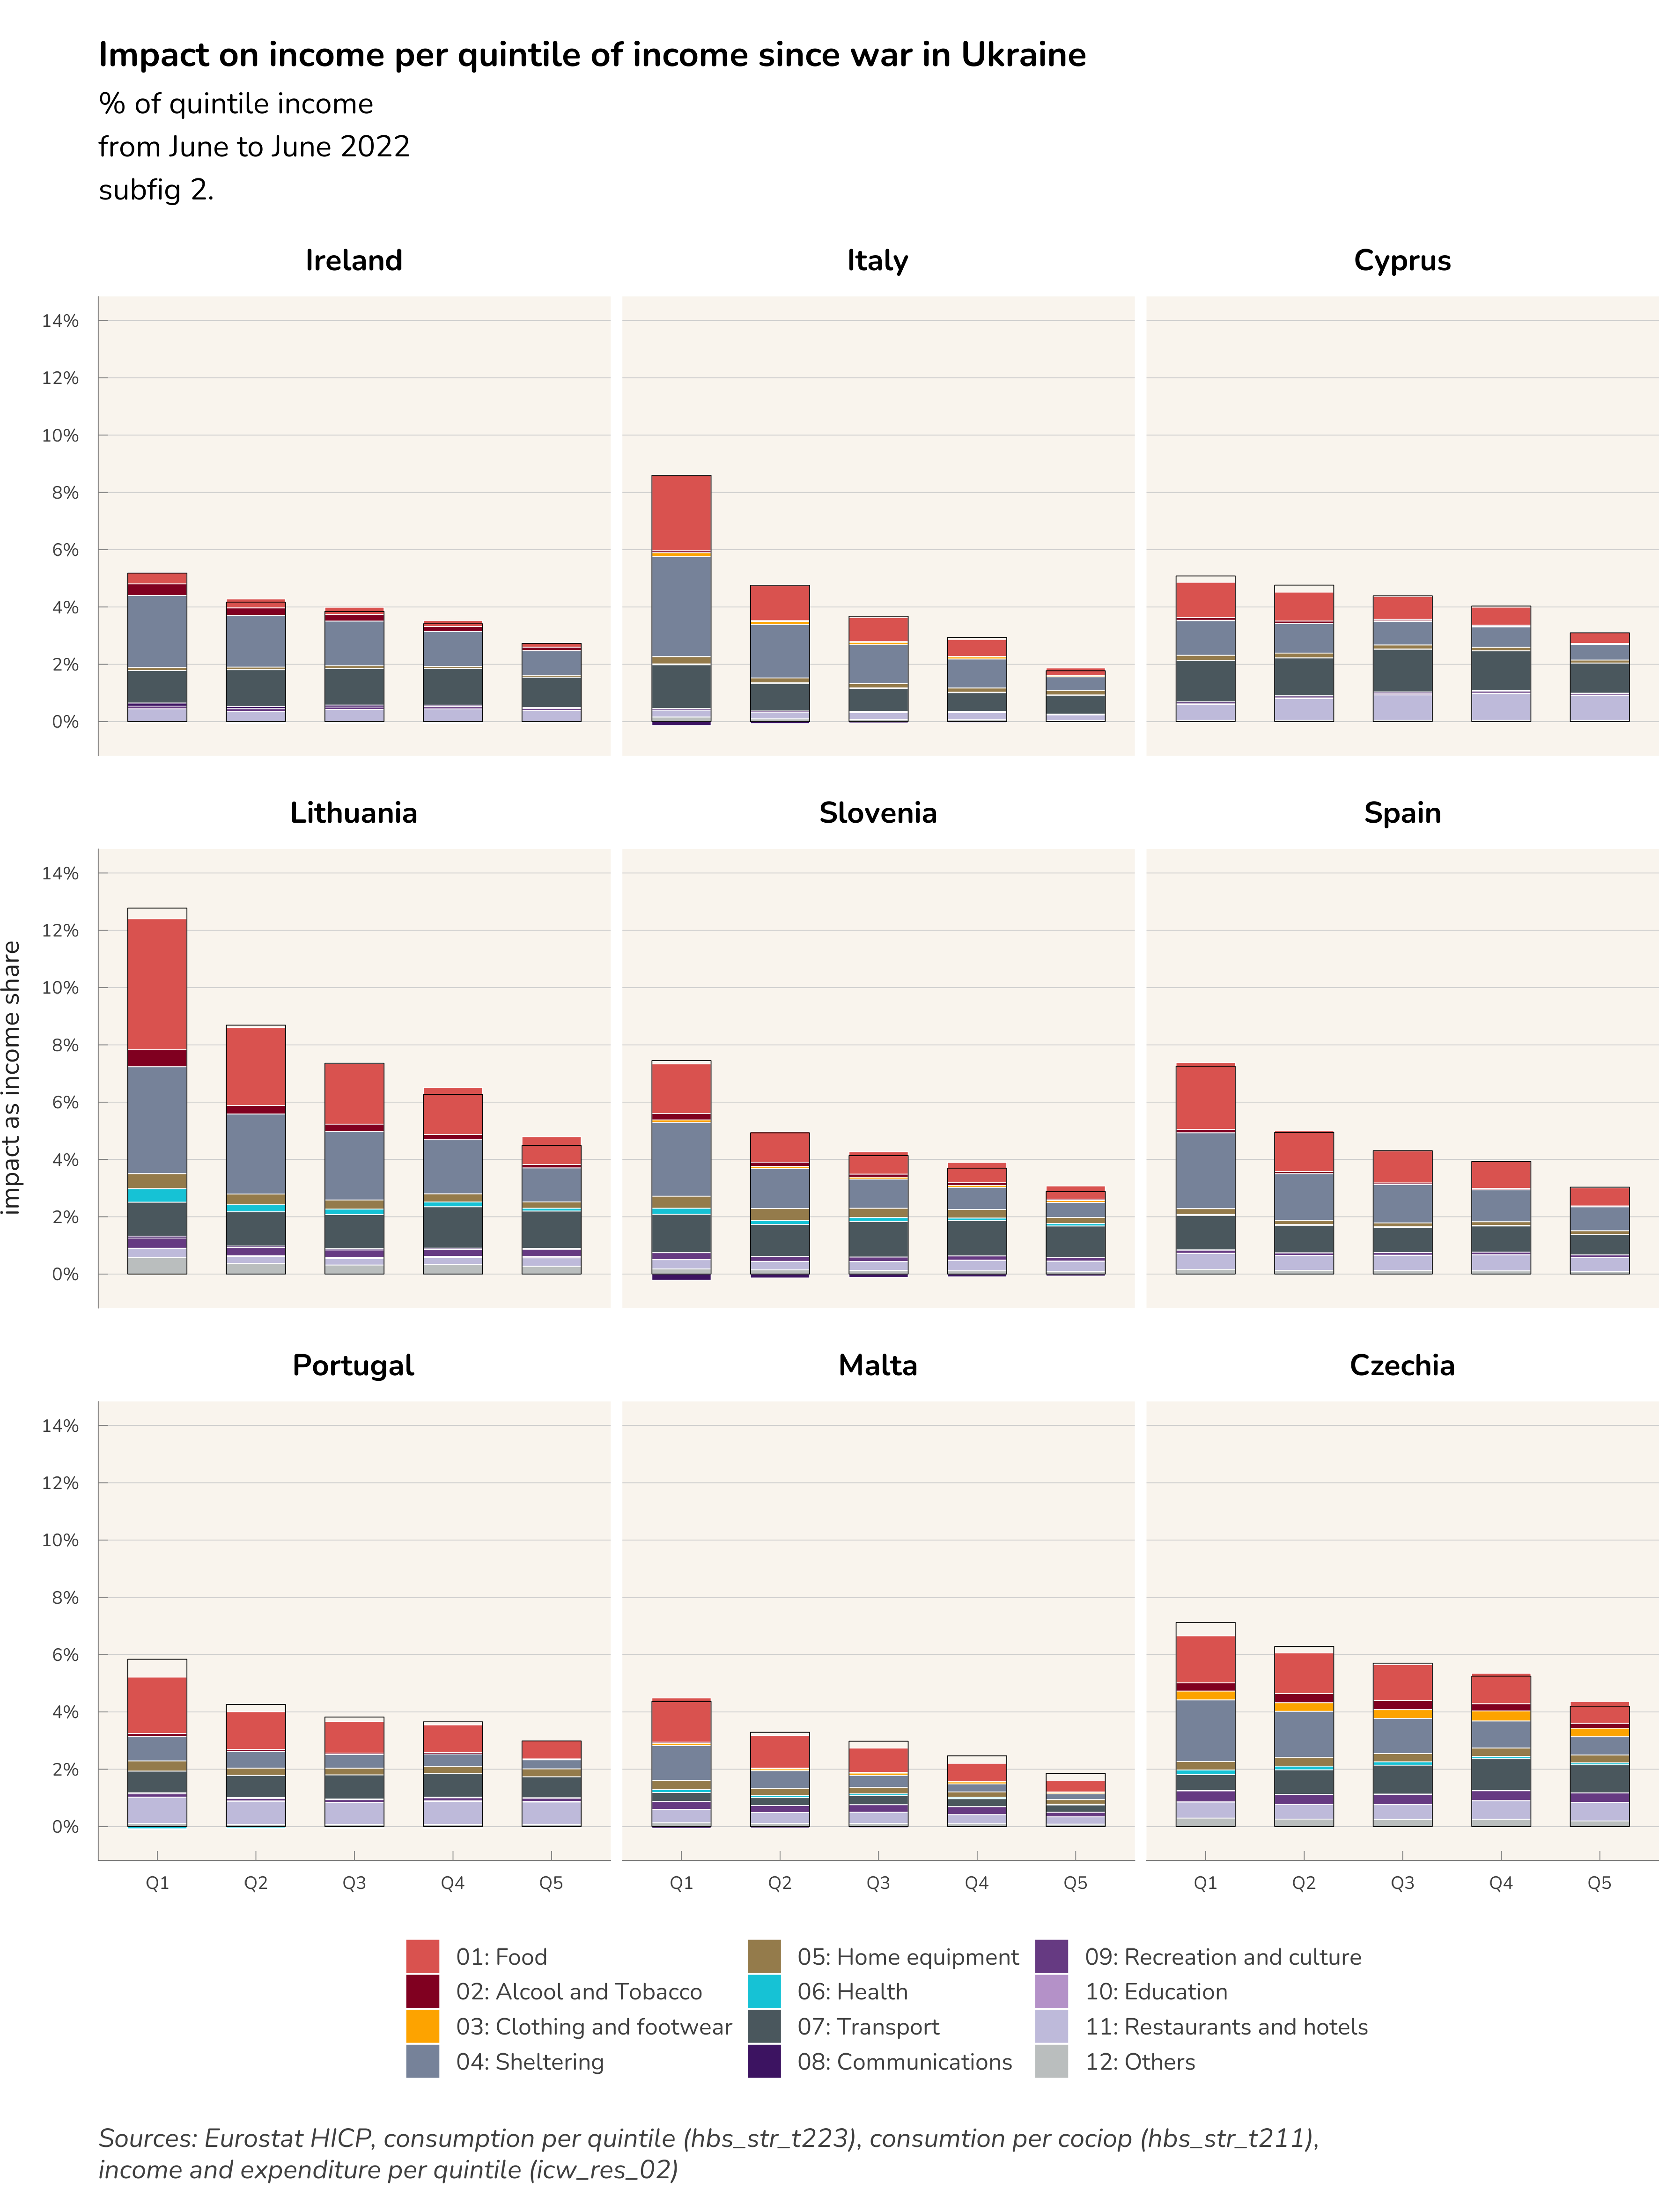
\includegraphics{../svg/coicop_l1_1y_2.png}

}

\end{figure}

\begin{figure}

\caption{Impact on income per quintile (3/3)}

{\centering 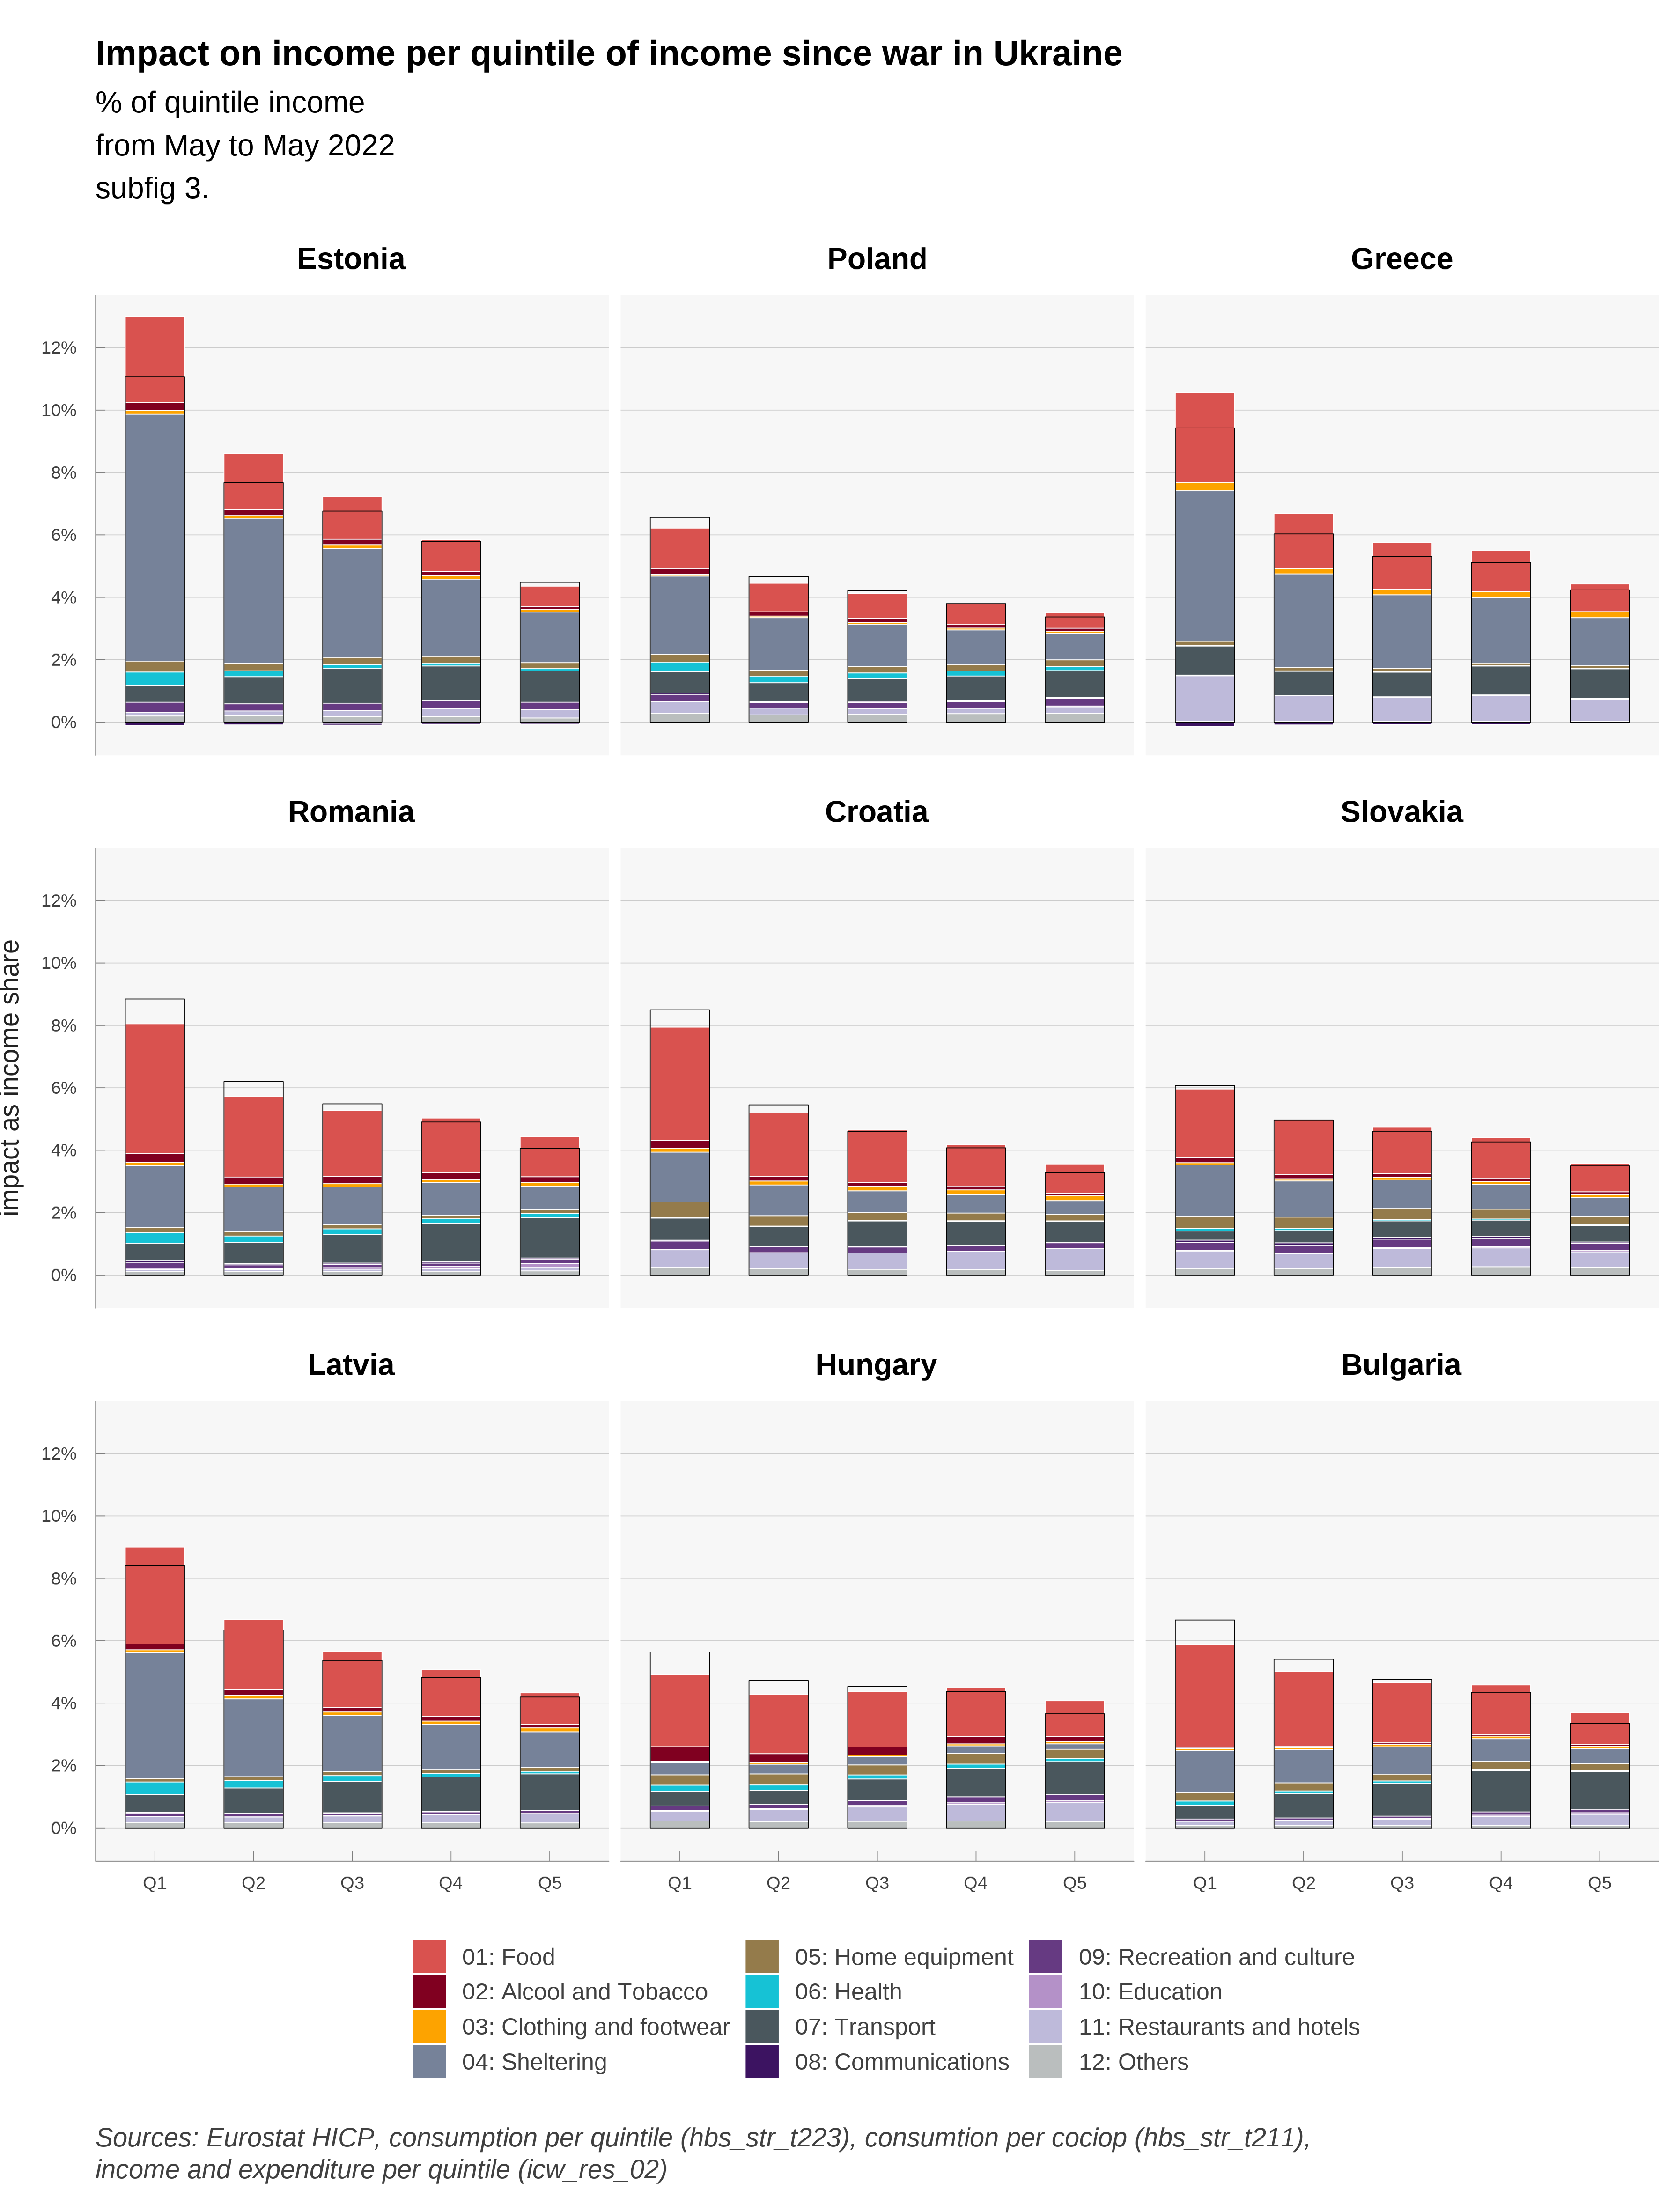
\includegraphics{../svg/coicop_l1_1y_3.png}

}

\end{figure}



\end{document}
